\chapter{Search I: Limits per mass category}
\label{app:search1}
 The asymptotic limits obtained with 2.6 $\textrm{fb}^{-1}$ of 13 TeV CMS data per mass and purity category. The largest significance is found at 2.8-3 TeV in the ZZ high-purity category, where one event at 3 TeV yields a local significance of 2.8 $\sigma$. A 3 parameter fit is the default background fit function for this category, however, a 2 parameter fit could also be used to describe these data. In Figure \ref{fig:Limits_ZZHP} we compare the limits and p-values obtained using a 2 parameter and a 3 parameter fit to describe the background in this category. The significance at 3 TeV is reduced from 2.8 to 1.5 $\sigma$ with a 2 parameter fit, reflecting the fact that the fit is poorly constrained in the high mass tail due to low statistics. The fit to data using both a 2 and 3 parameter fit is the ZZHP category is shown in Figure~\ref{fig:app:ZZHP2vs3p}.

\begin{figure}[h!]
\centering
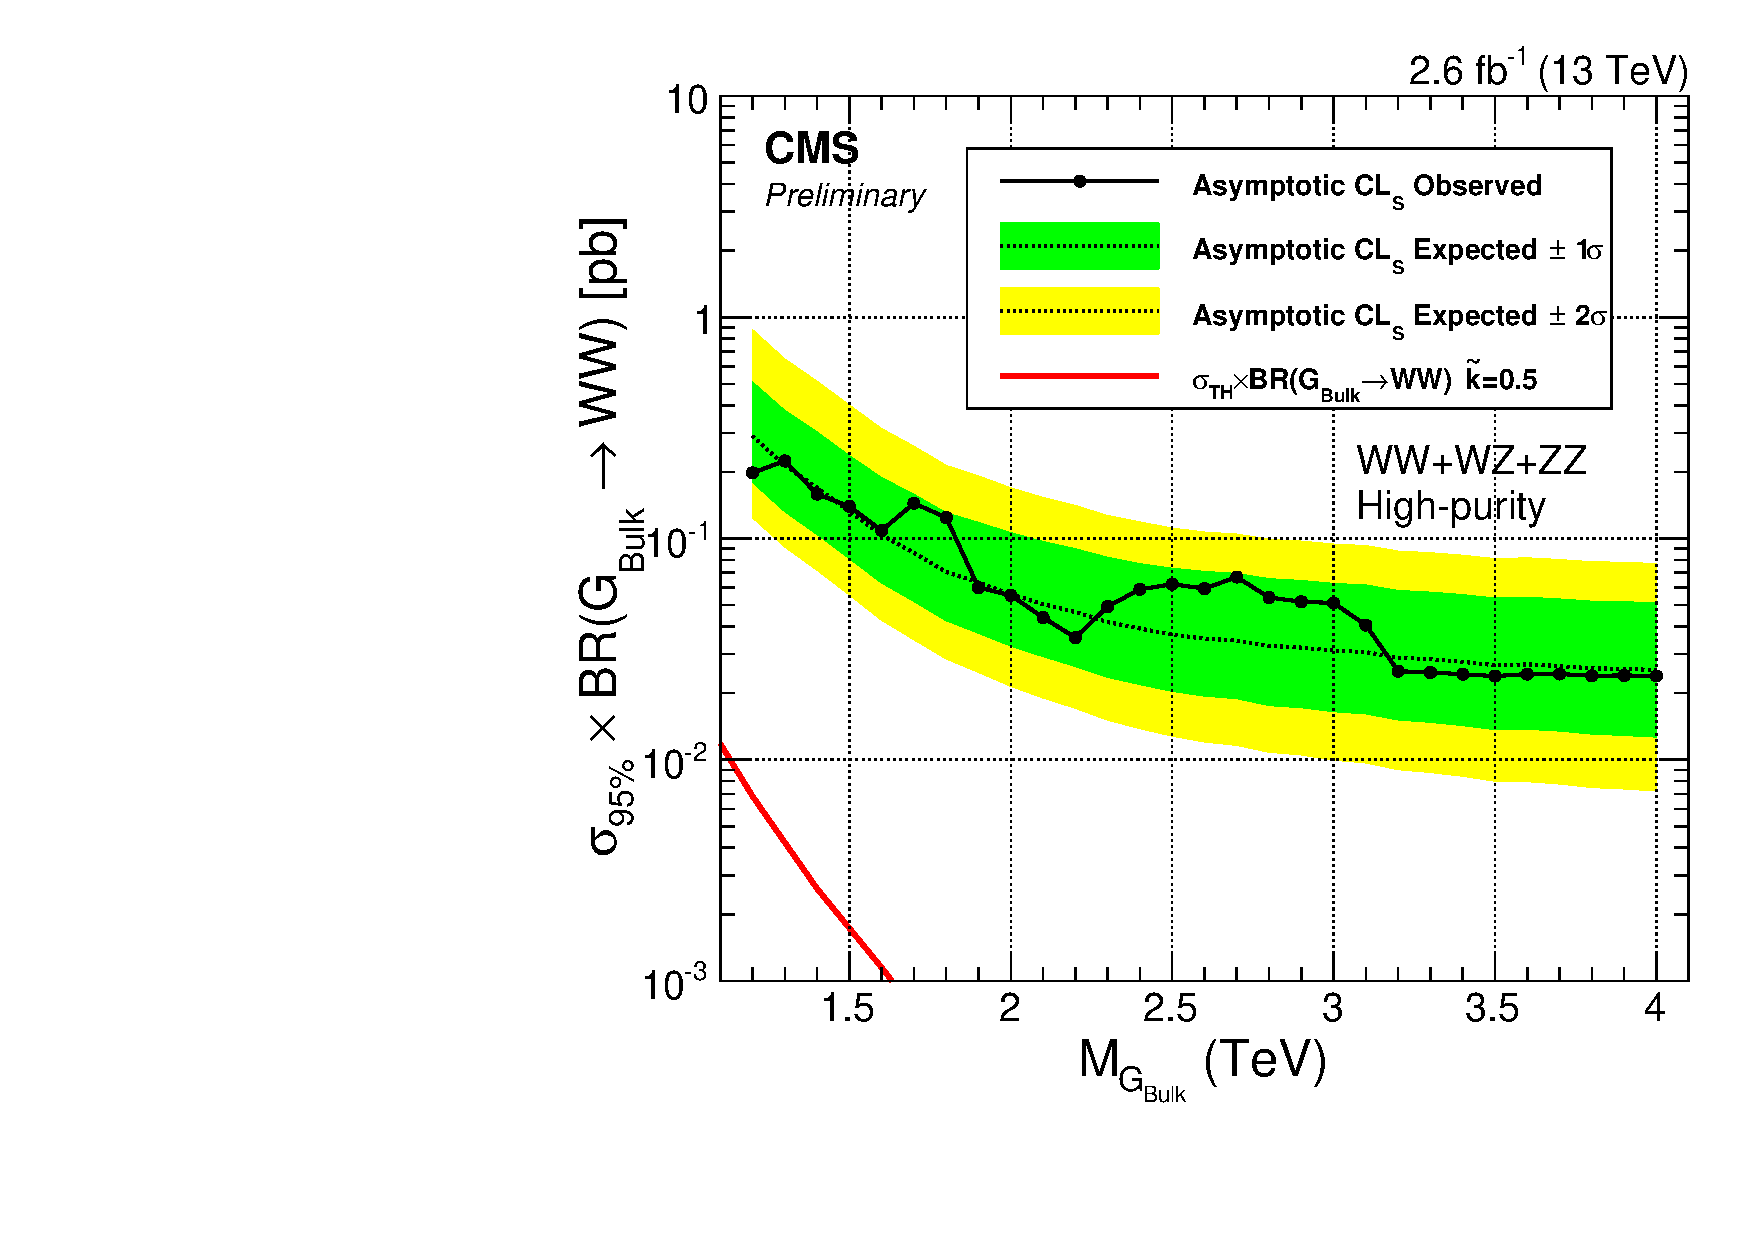
\includegraphics[width=0.32\textwidth]{figures/analysis/search1/AN-15-211/limits/brazilianFlag_BulkWW_VVHP_new_combined_purity_13TeV_wPDF.pdf}
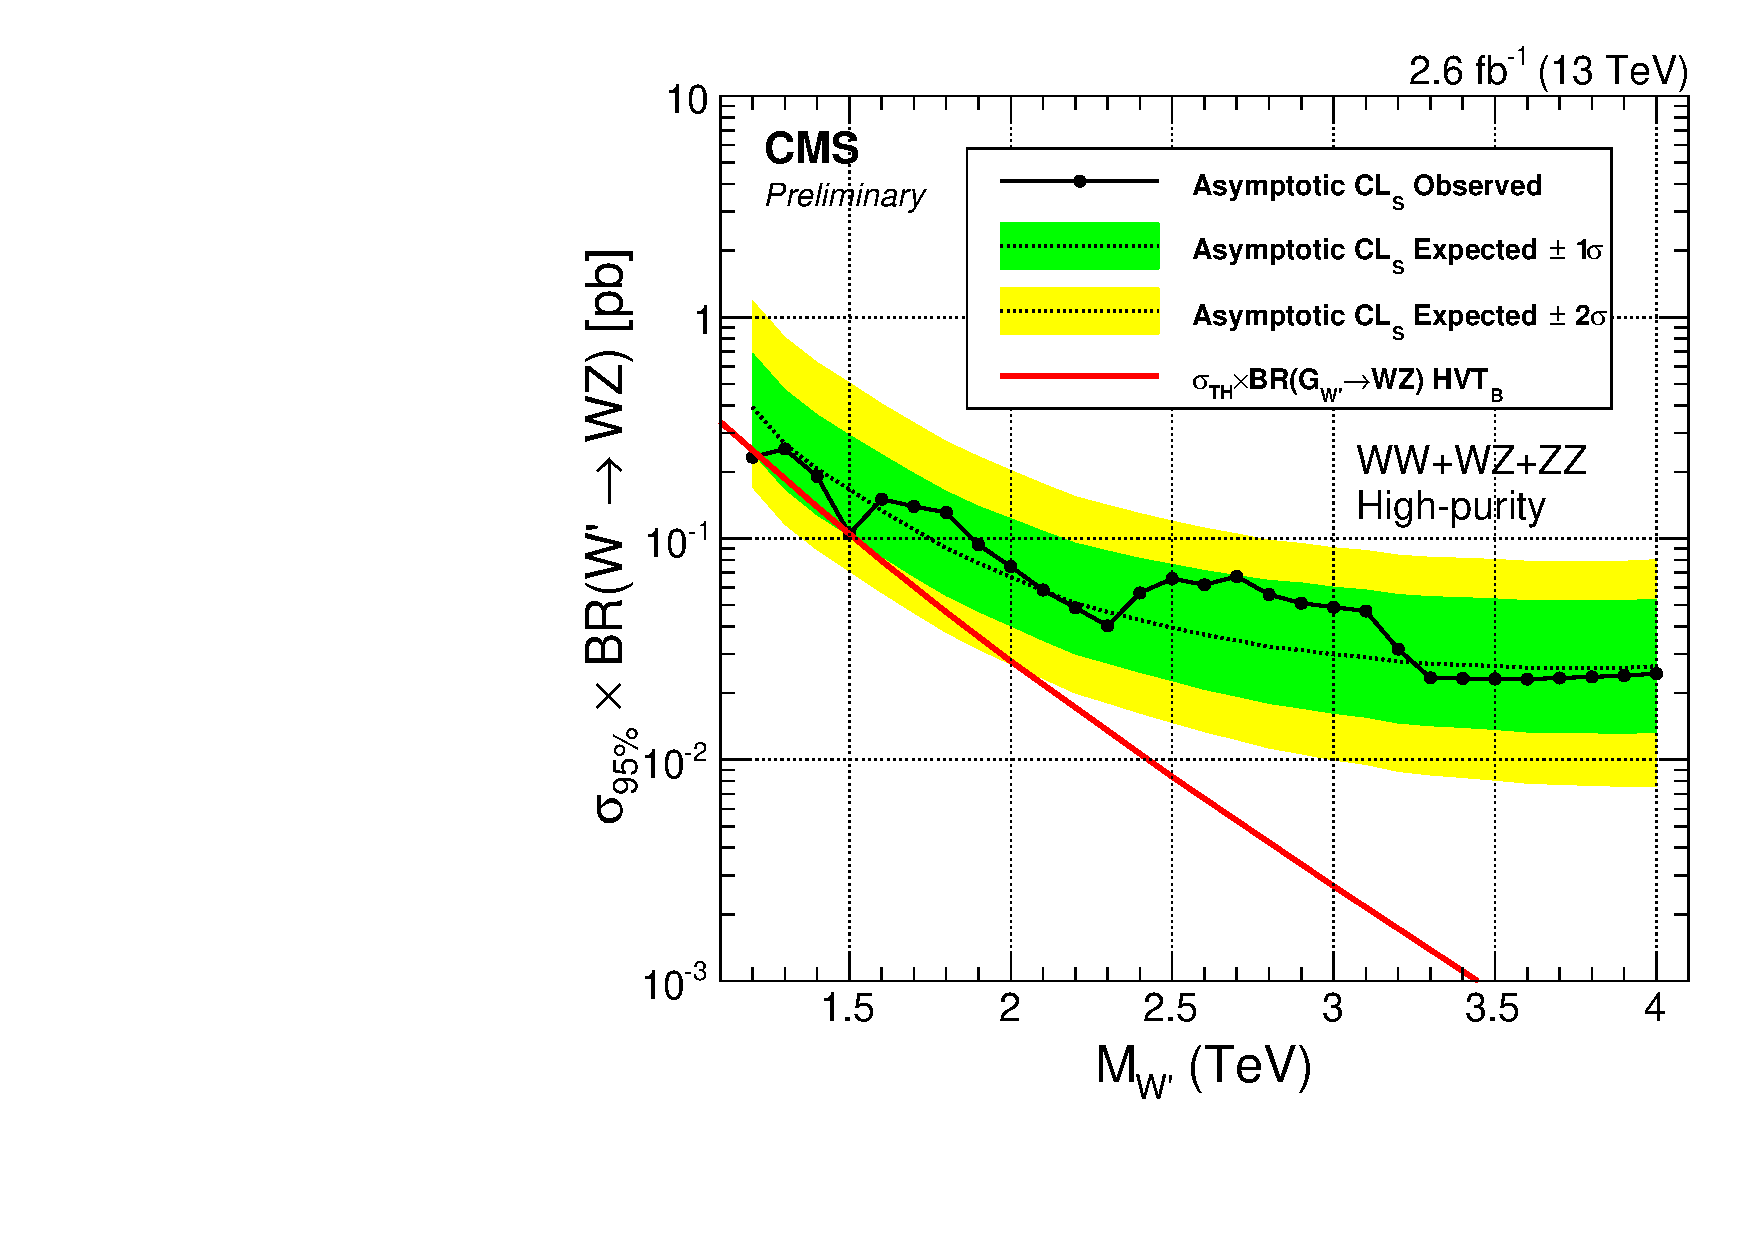
\includegraphics[width=0.32\textwidth]{figures/analysis/search1/AN-15-211/limits/brazilianFlag_WZ_VVHP_new_combined_purity_13TeV_wPDF.pdf}
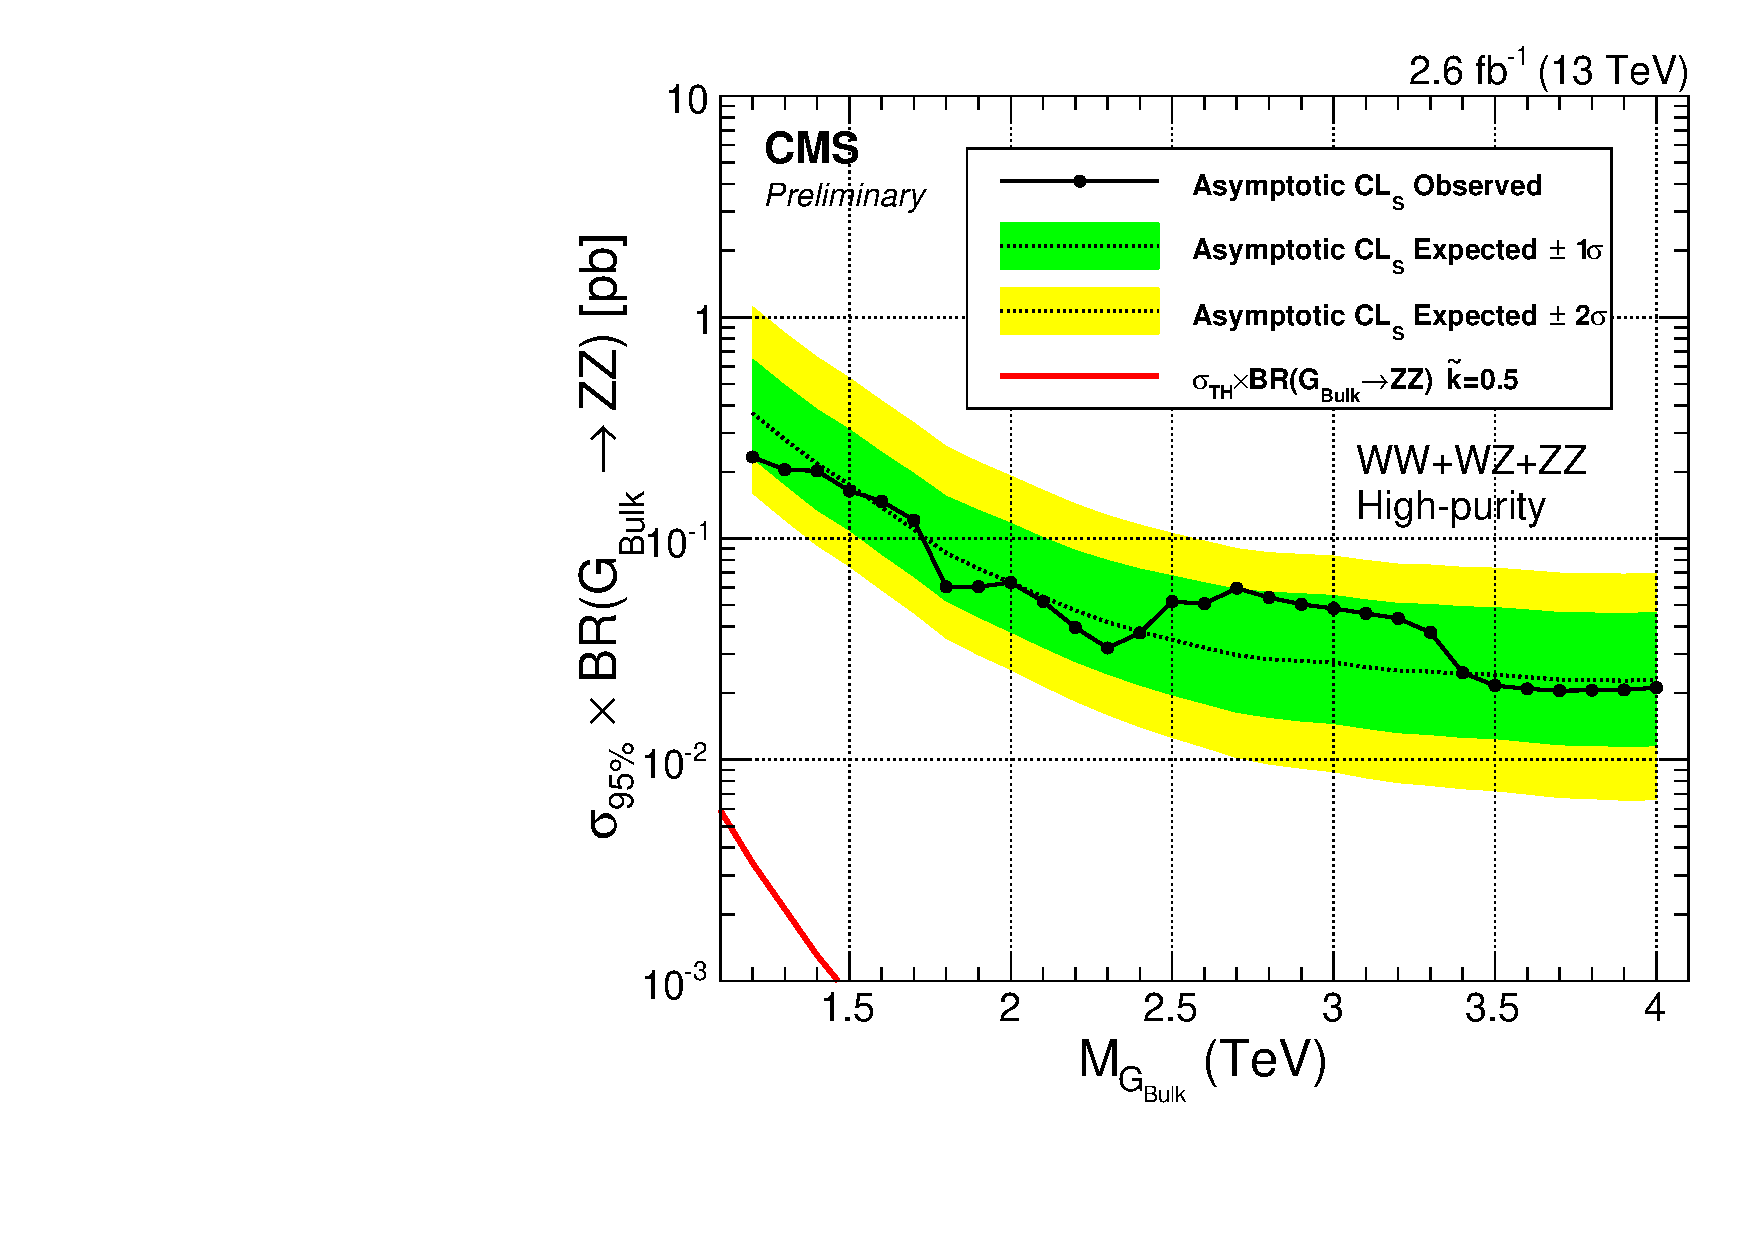
\includegraphics[width=0.32\textwidth]{figures/analysis/search1/AN-15-211/limits/brazilianFlag_BulkZZ_VVHP_new_combined_purity_13TeV_wPDF.pdf}\\
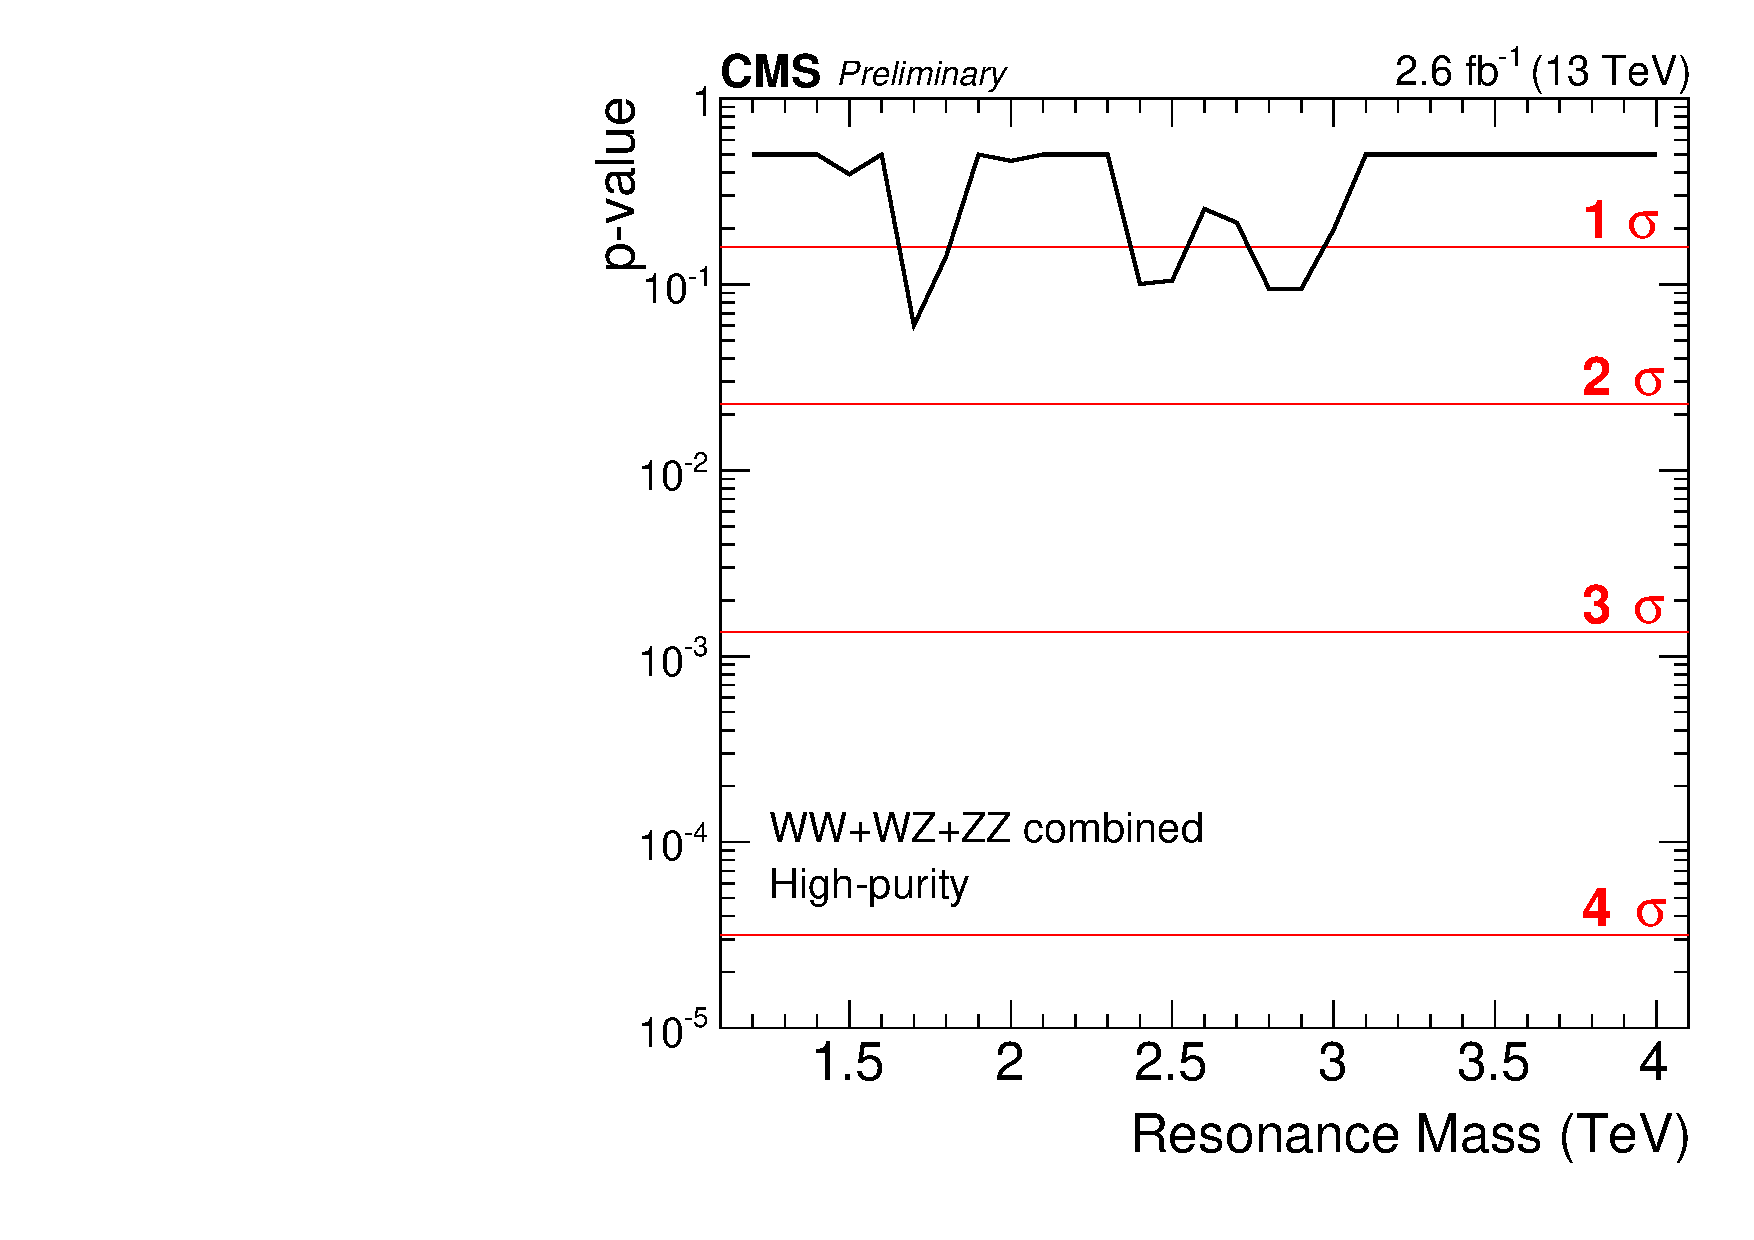
\includegraphics[width=0.32\textwidth]{figures/analysis/search1/AN-15-211/pvalues/pvalue_BulkWWinVVnew_high_purity.pdf}
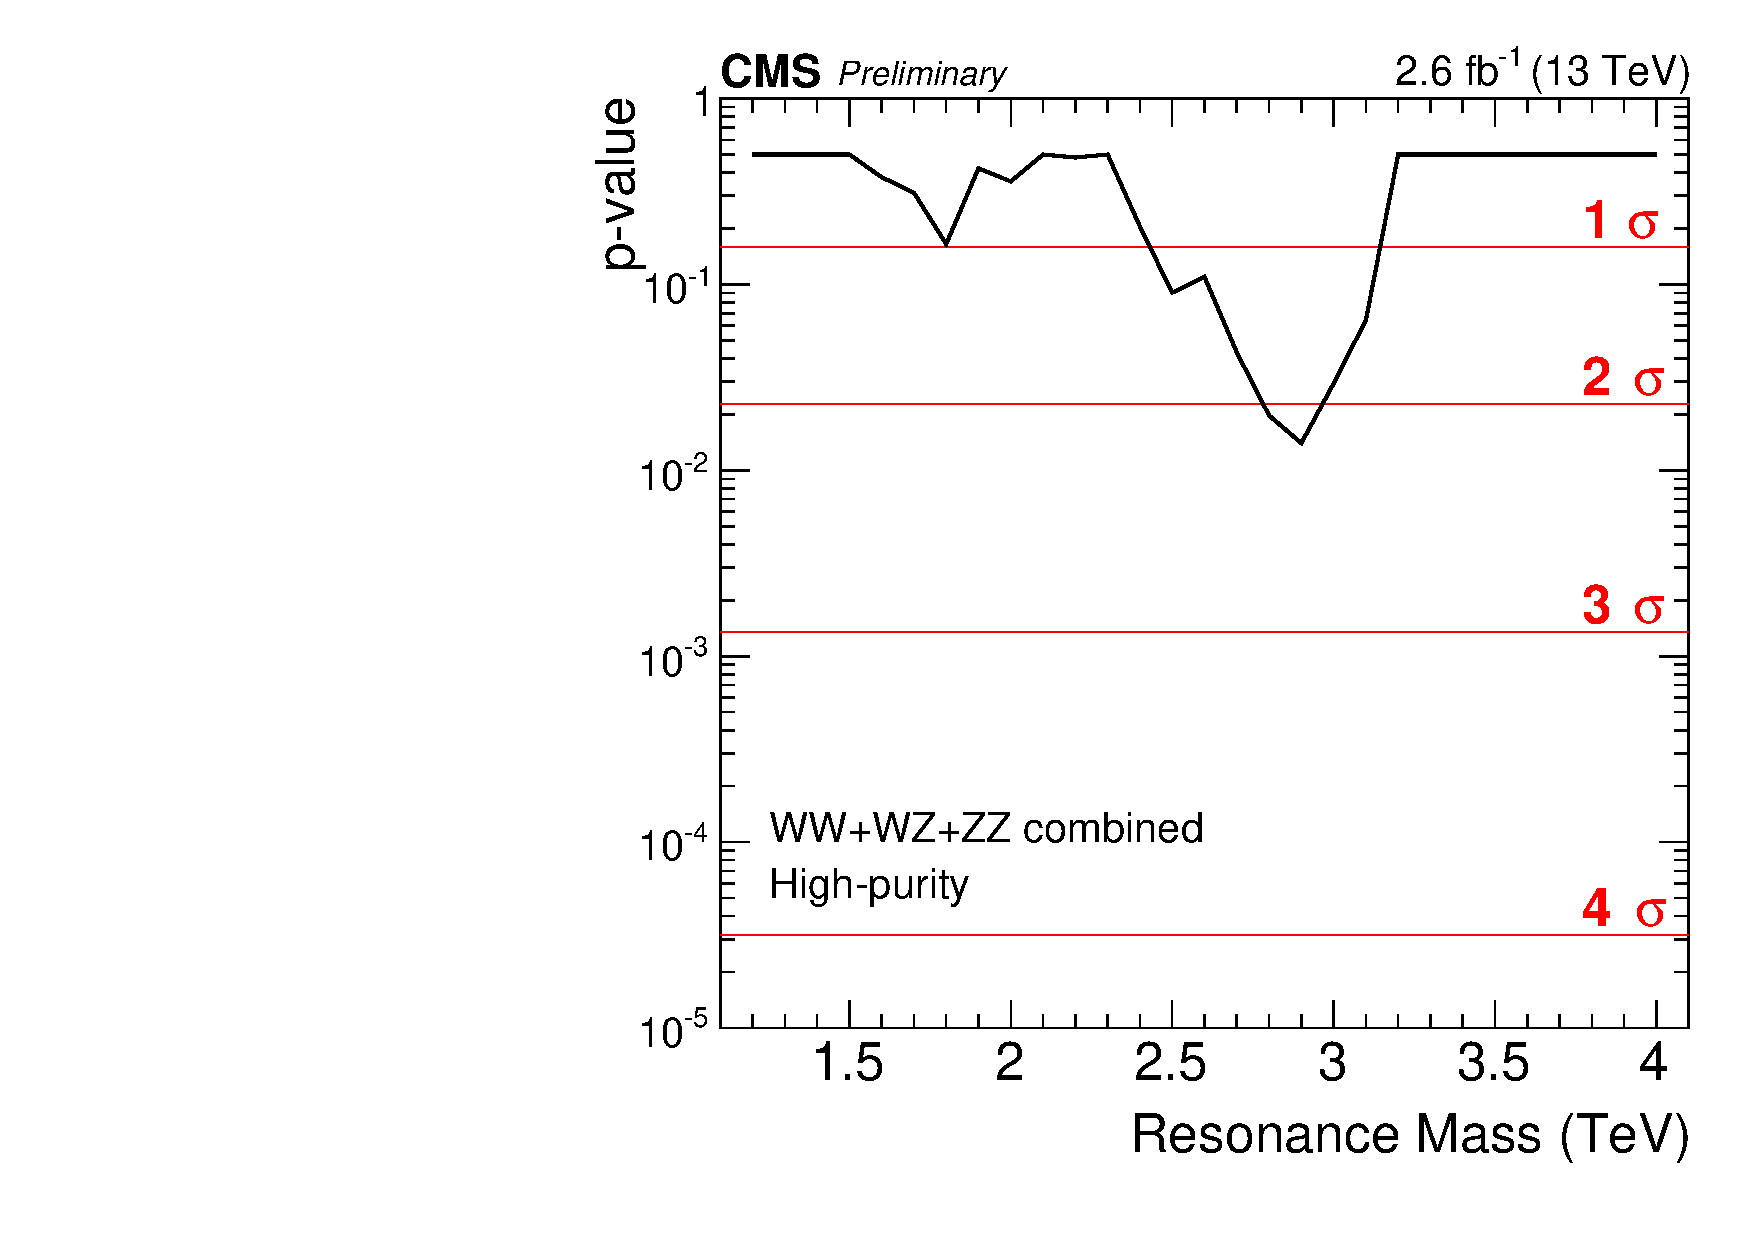
\includegraphics[width=0.32\textwidth]{figures/analysis/search1/AN-15-211/pvalues/pvalue_WZinVVnew_high_purity.pdf}
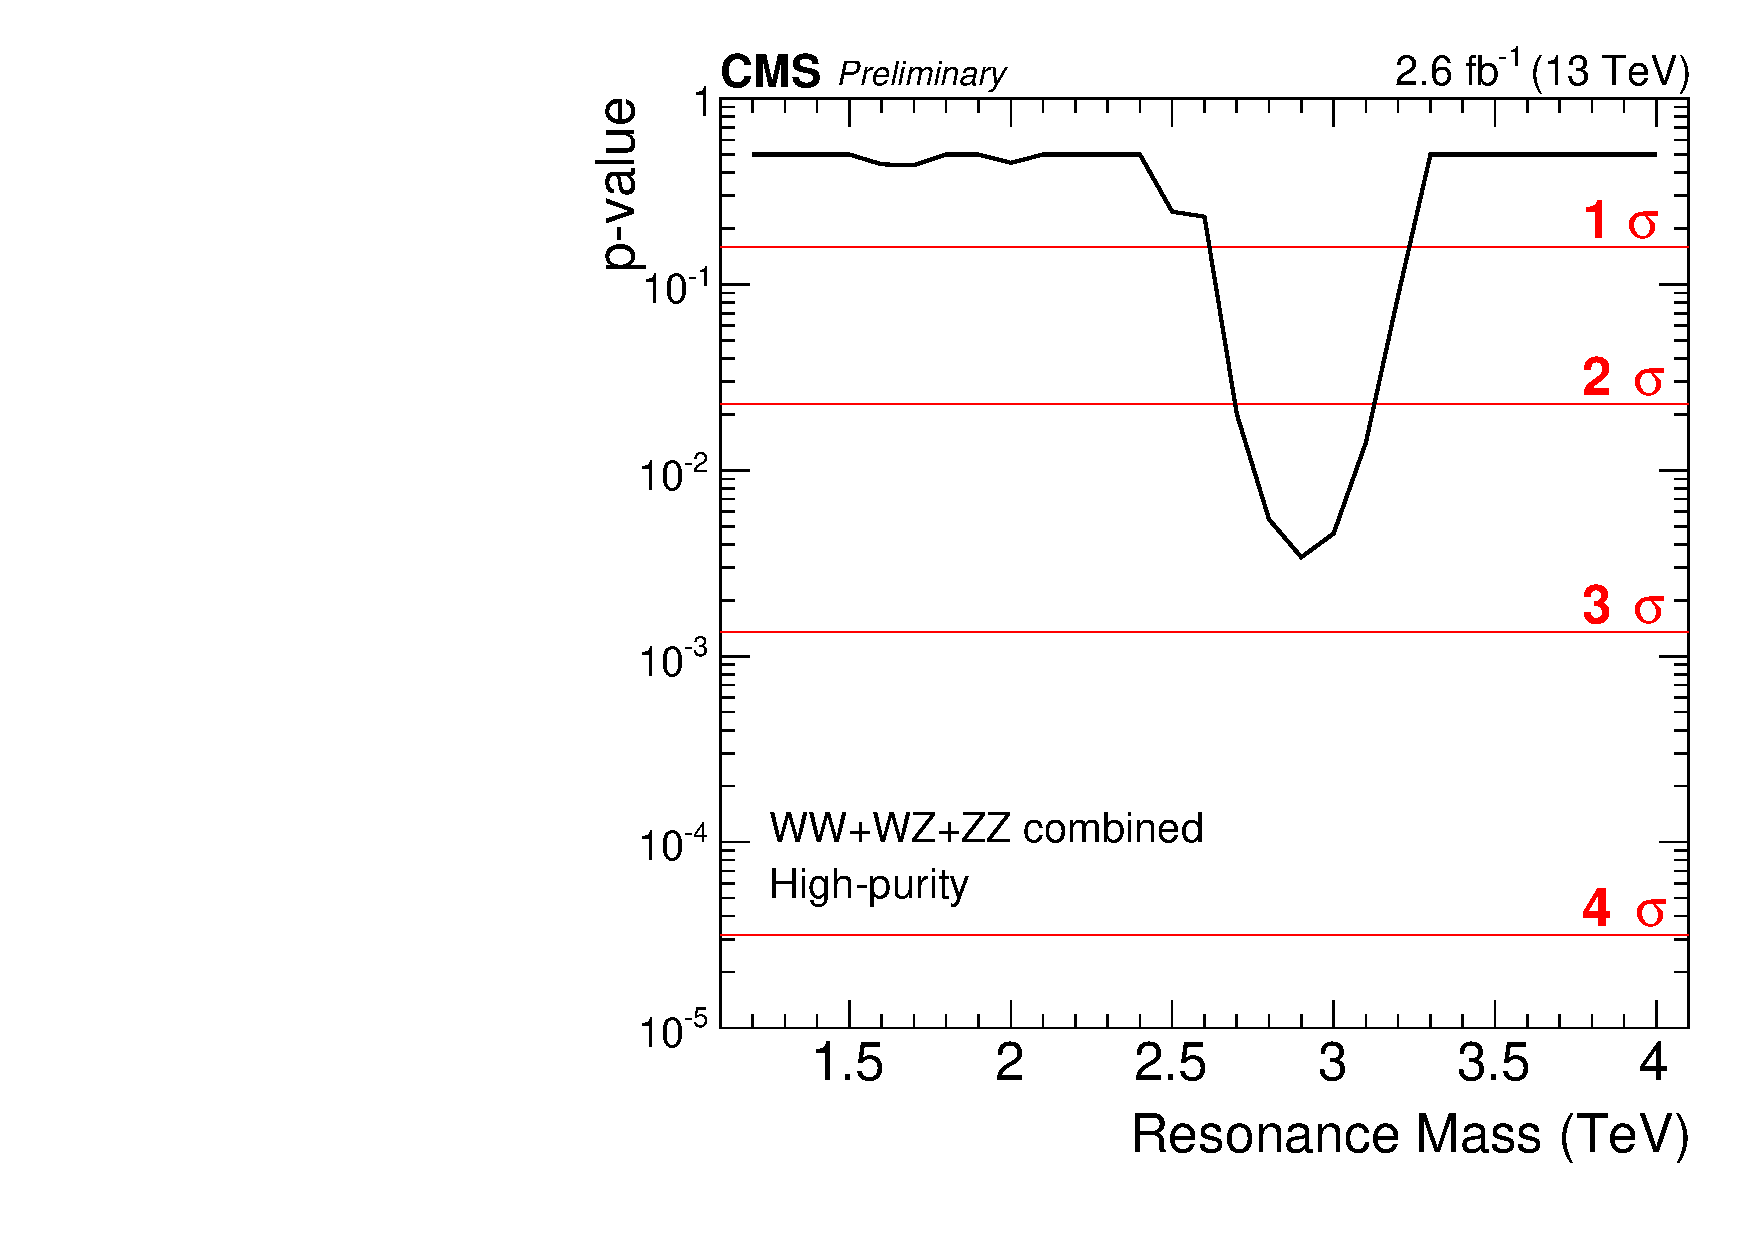
\includegraphics[width=0.32\textwidth]{figures/analysis/search1/AN-15-211/pvalues/pvalue_BulkZZinVVnew_high_purity.pdf}
\caption{Expected/observed limits and corresponding p-values obtained in the high purity category using 2.6 $\textrm{fb}^{-1}$ of CMS data. Here for a Bulk $G\rightarrow WW$ (left), $W'\rightarrow WZ$ (middle) and $G\rightarrow ZZ$ (right) signal.}
\label{fig:searchI:Limits_HP}
\end{figure}


\begin{figure}[h!]
\centering
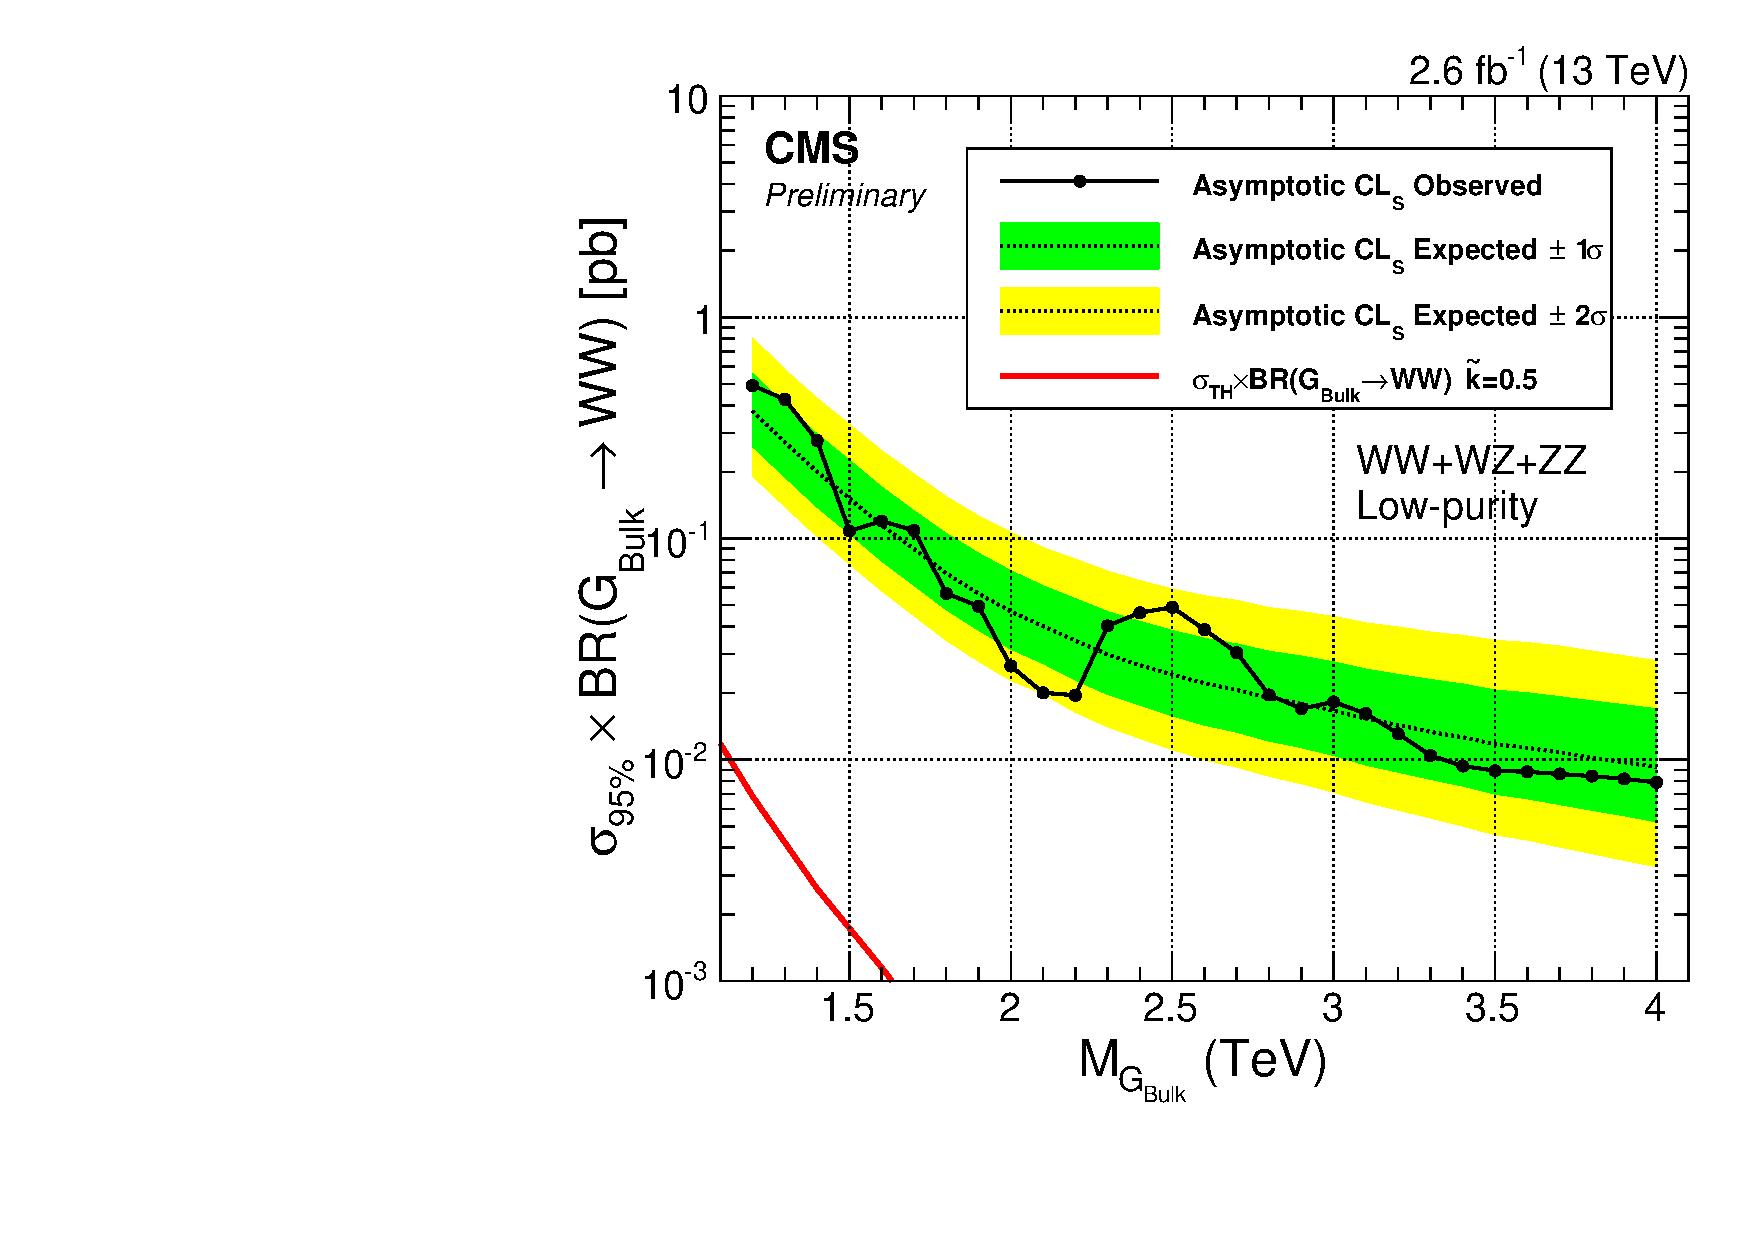
\includegraphics[width=0.32\textwidth]{figures/analysis/search1/AN-15-211/limits/brazilianFlag_BulkWW_VVLP_new_combined_purity_13TeV_wPDF.pdf}
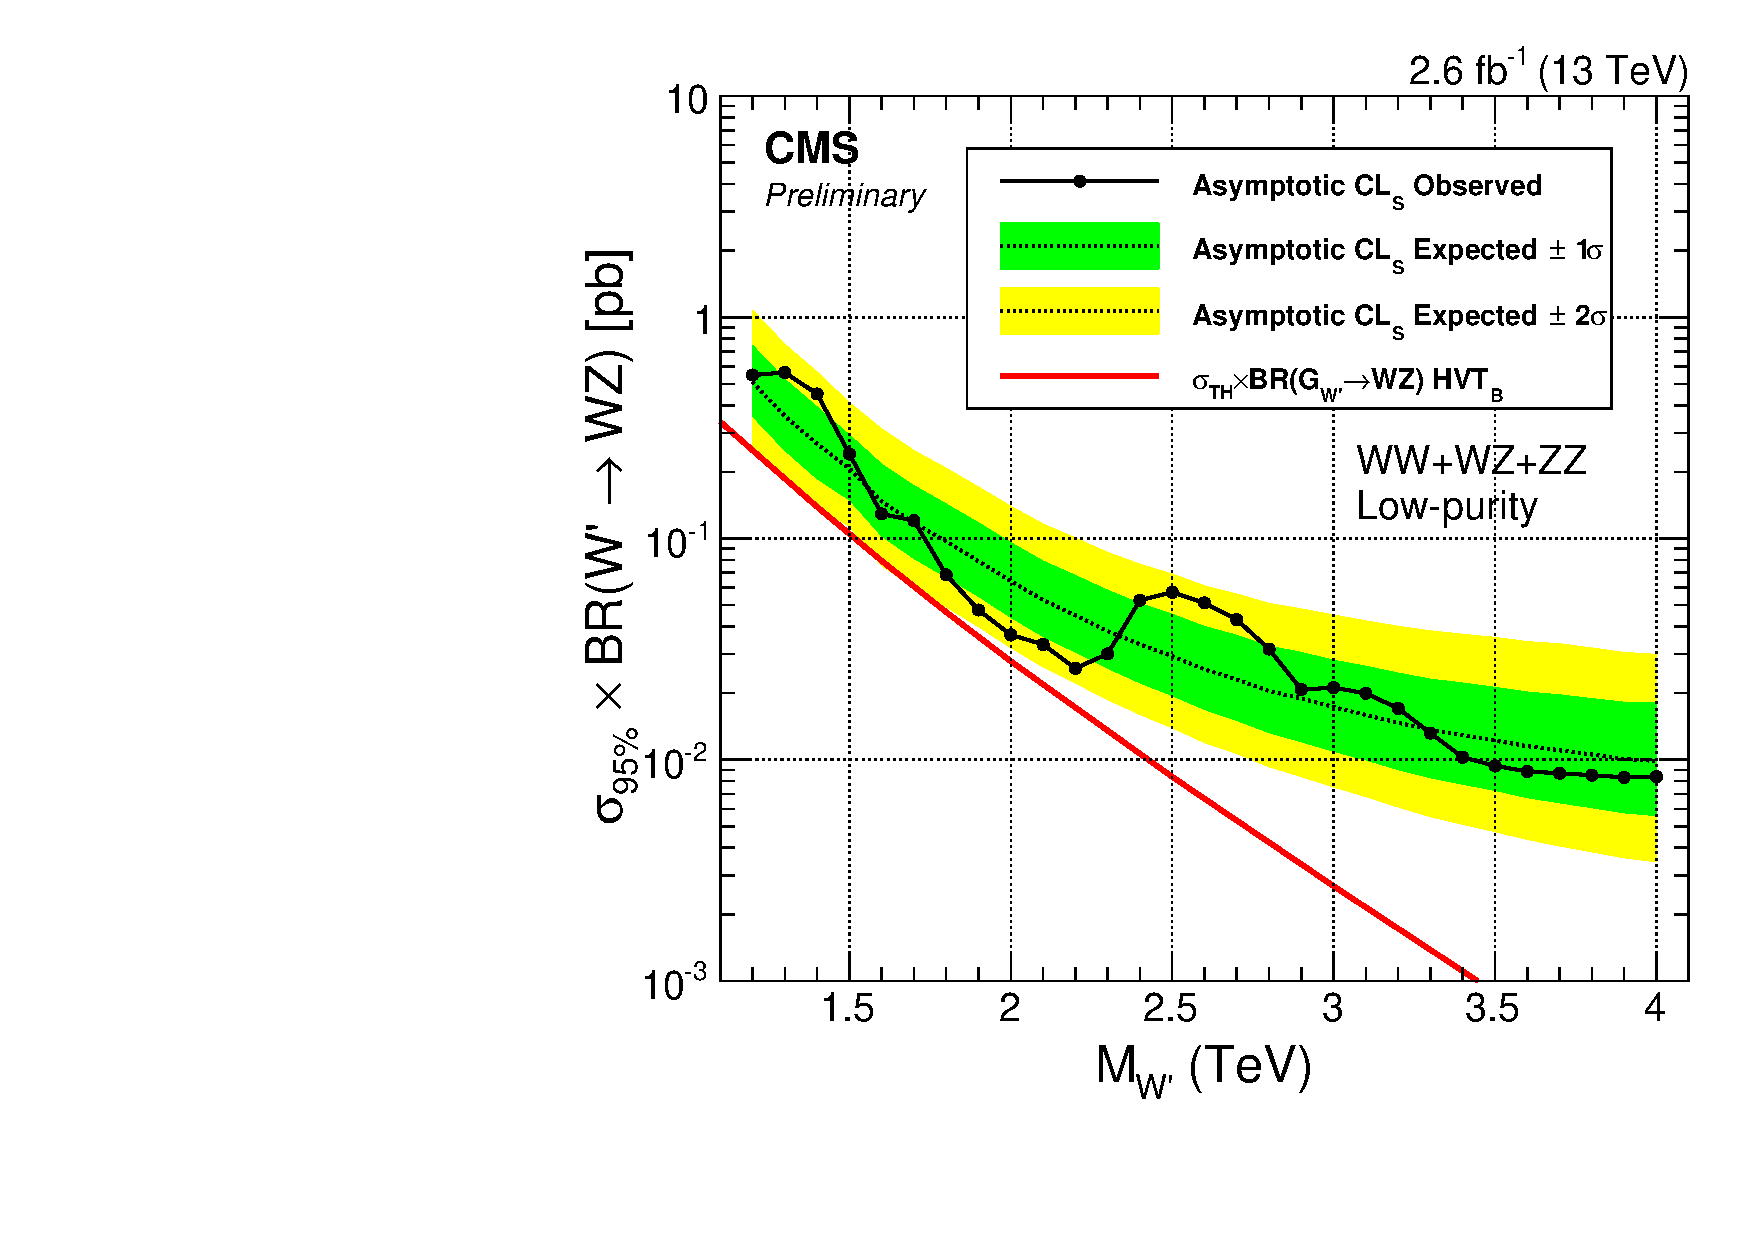
\includegraphics[width=0.32\textwidth]{figures/analysis/search1/AN-15-211/limits/brazilianFlag_WZ_VVLP_new_combined_purity_13TeV_wPDF.pdf}
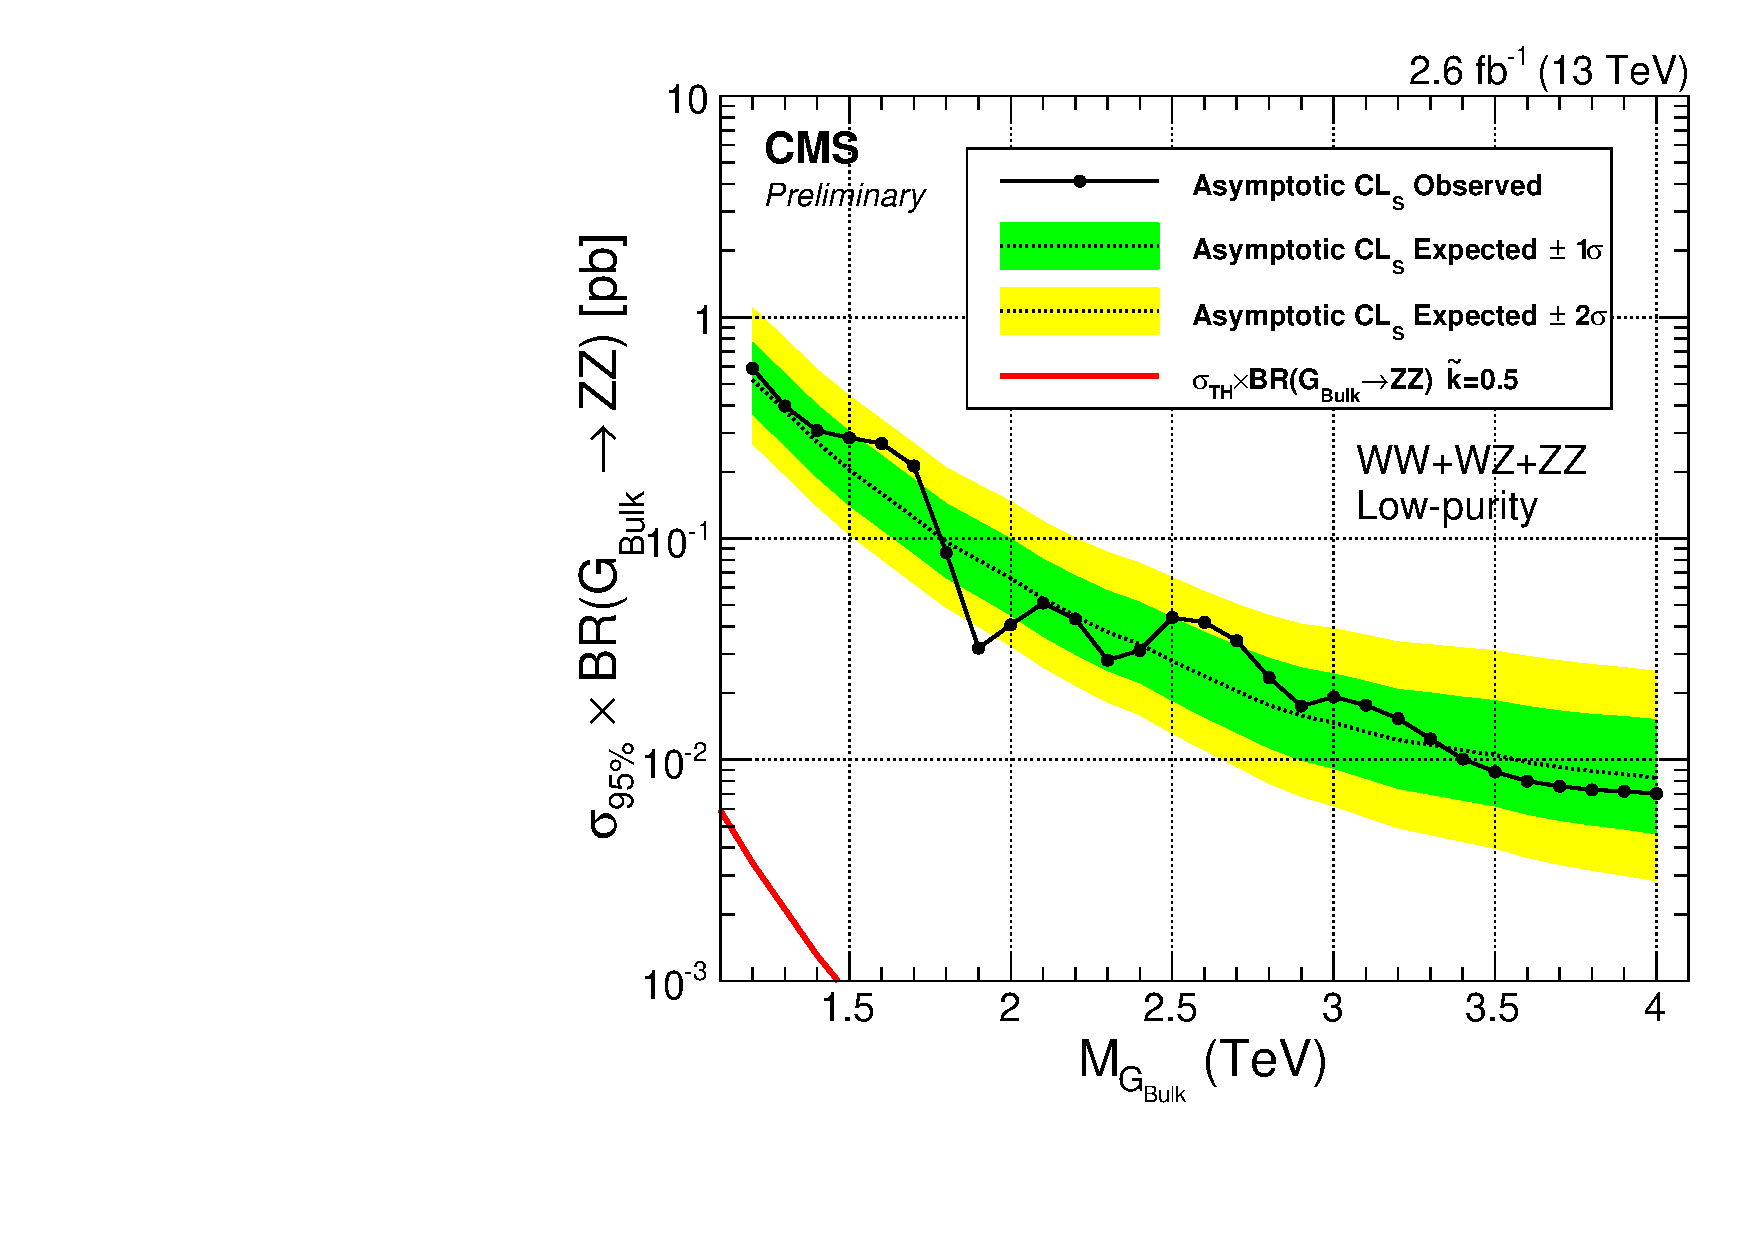
\includegraphics[width=0.32\textwidth]{figures/analysis/search1/AN-15-211/limits/brazilianFlag_BulkZZ_VVLP_new_combined_purity_13TeV_wPDF.pdf}\\
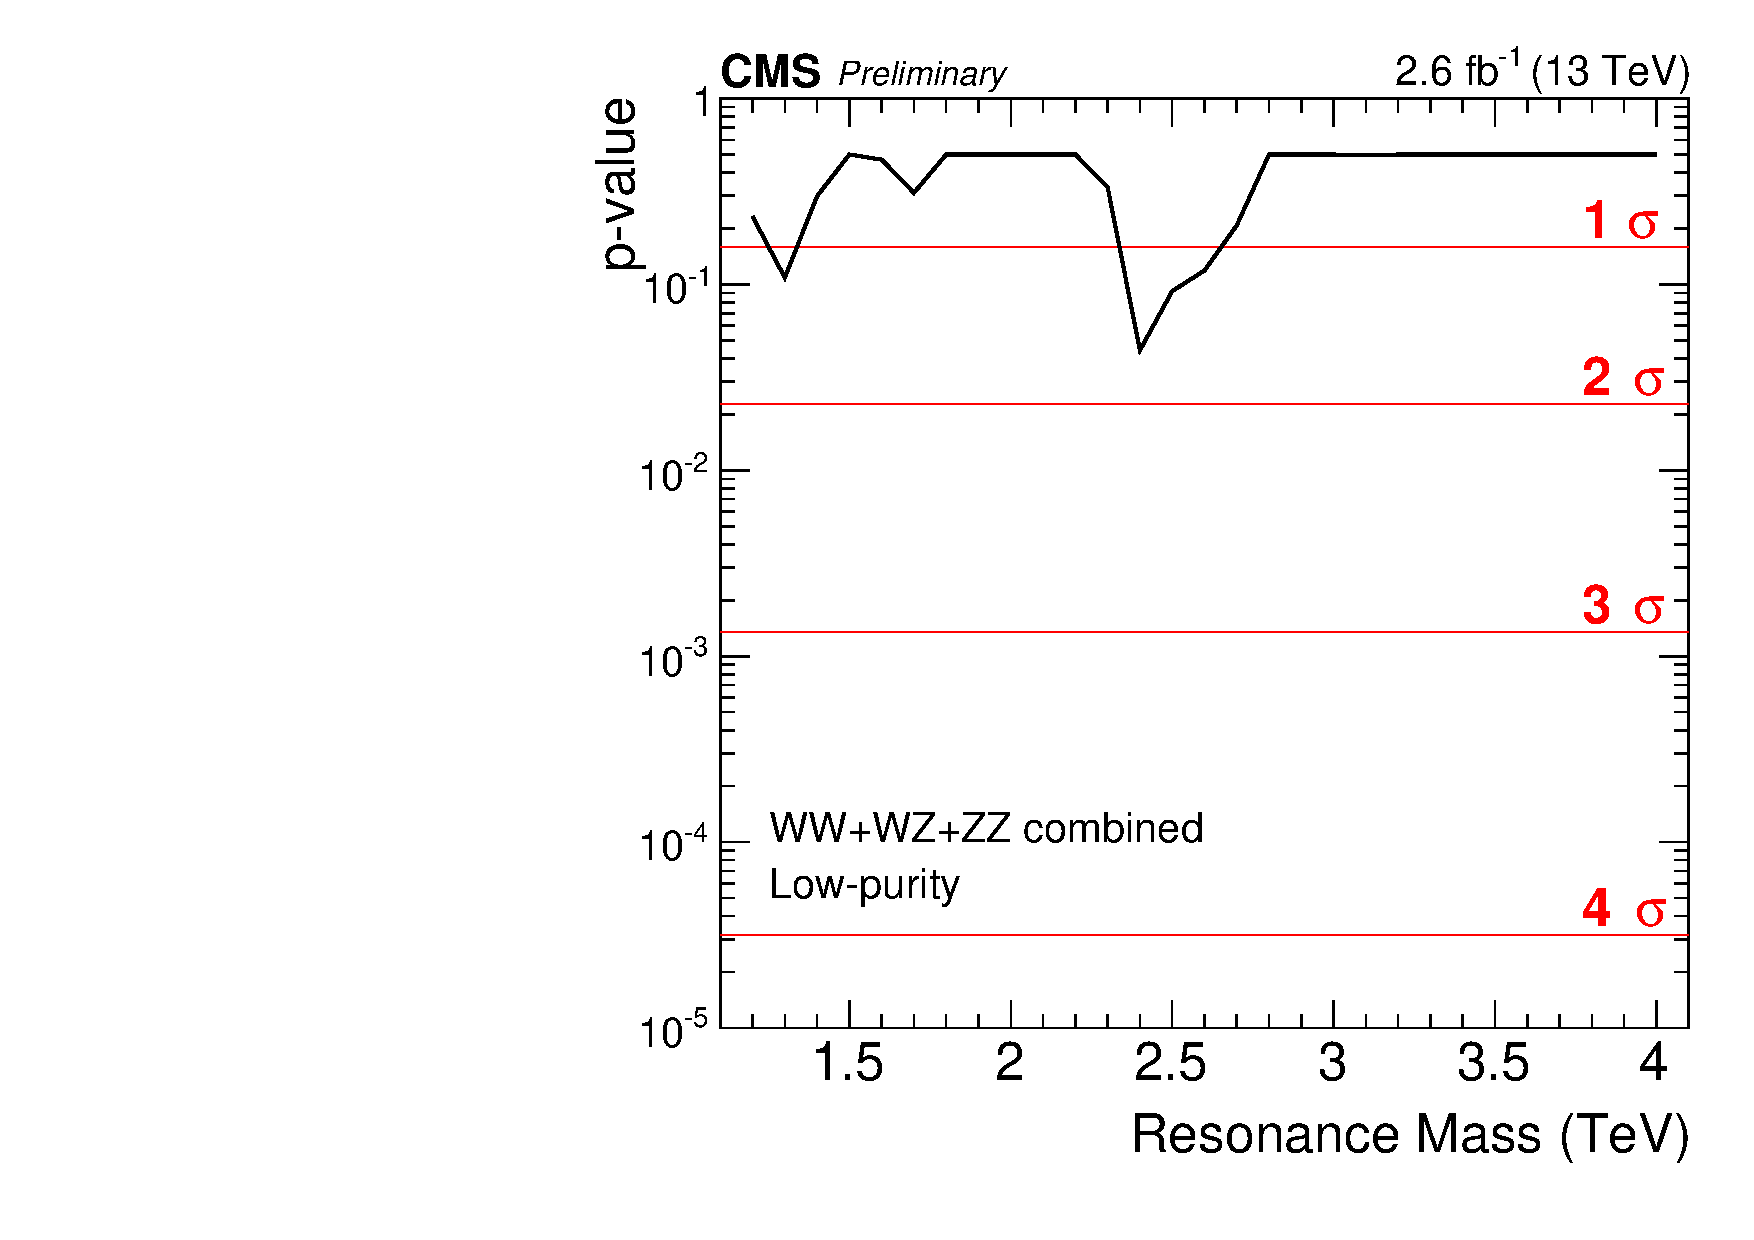
\includegraphics[width=0.32\textwidth]{figures/analysis/search1/AN-15-211/pvalues/pvalue_BulkWWinVVnew_low_purity.pdf}
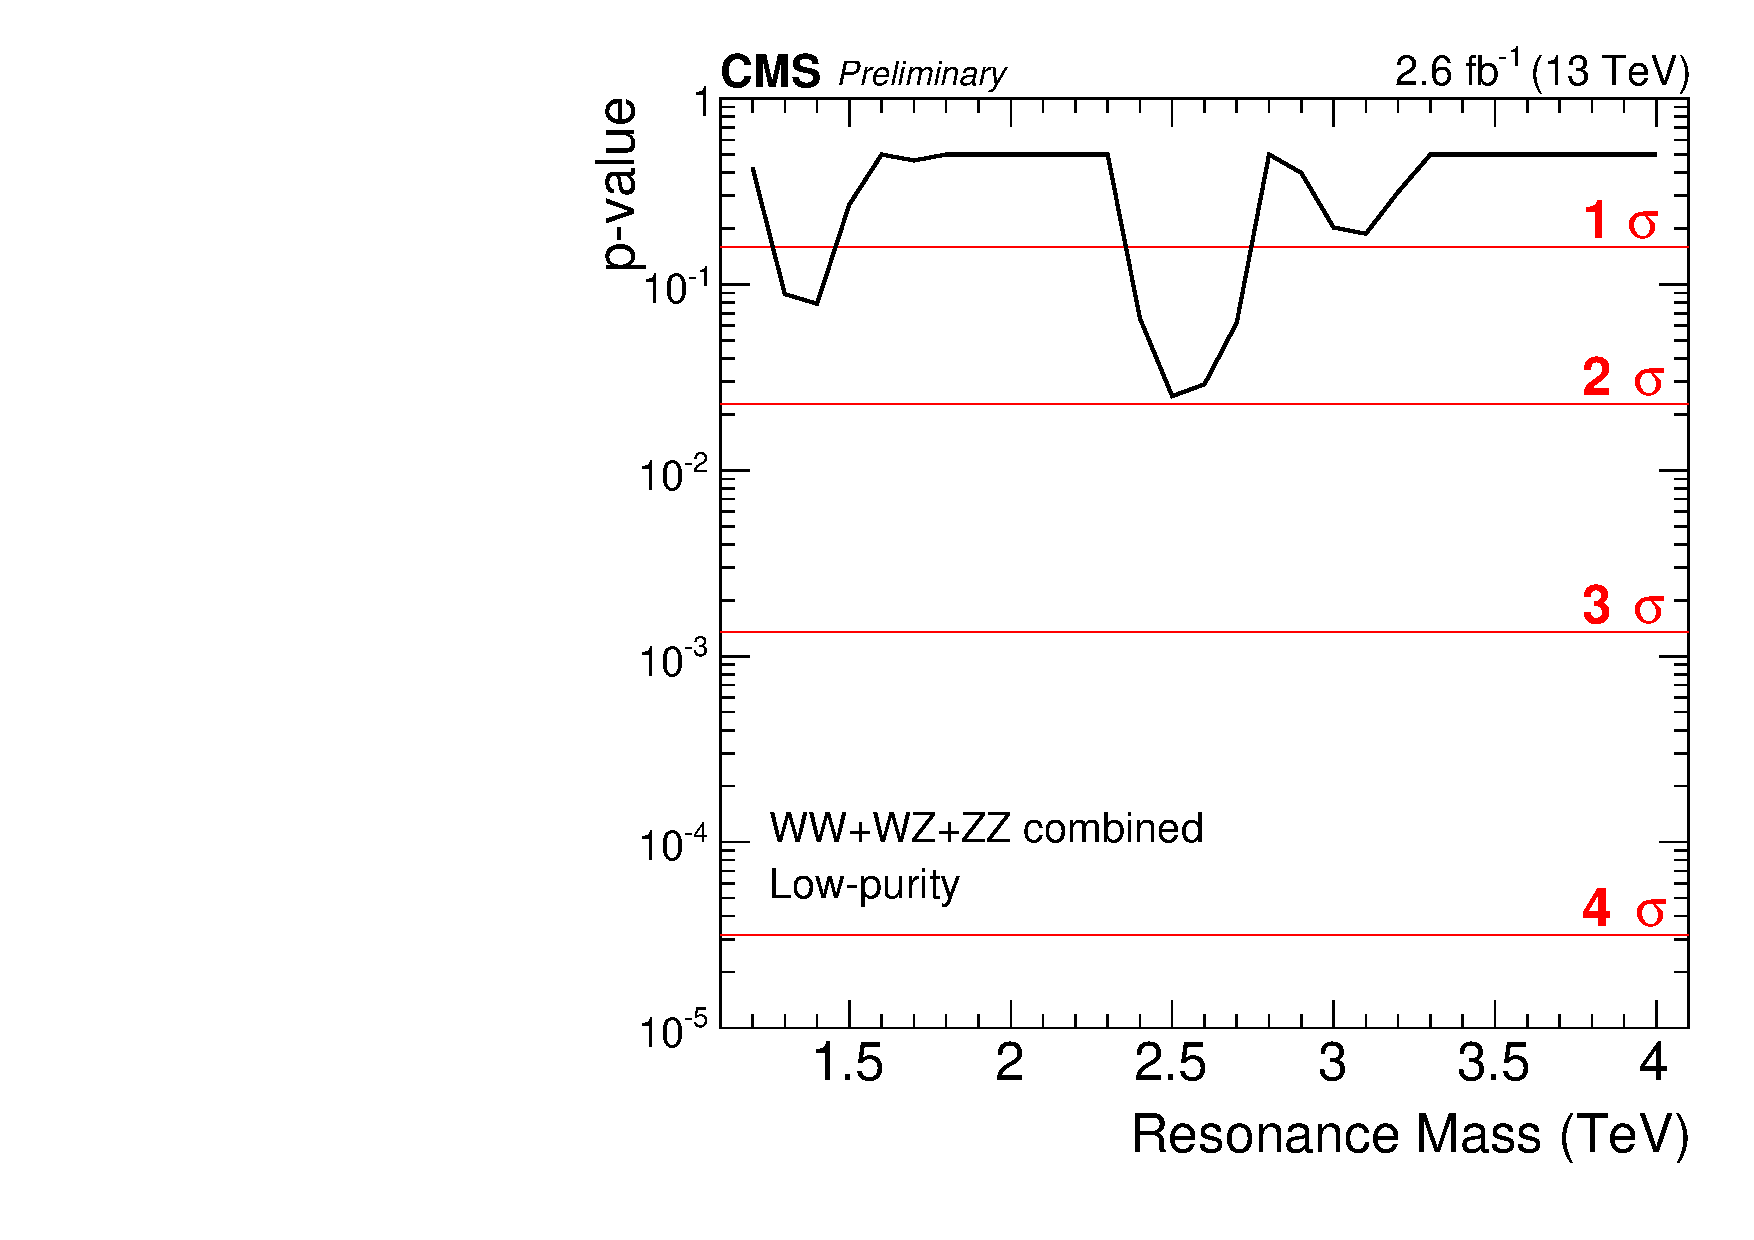
\includegraphics[width=0.32\textwidth]{figures/analysis/search1/AN-15-211/pvalues/pvalue_WZinVVnew_low_purity.pdf}
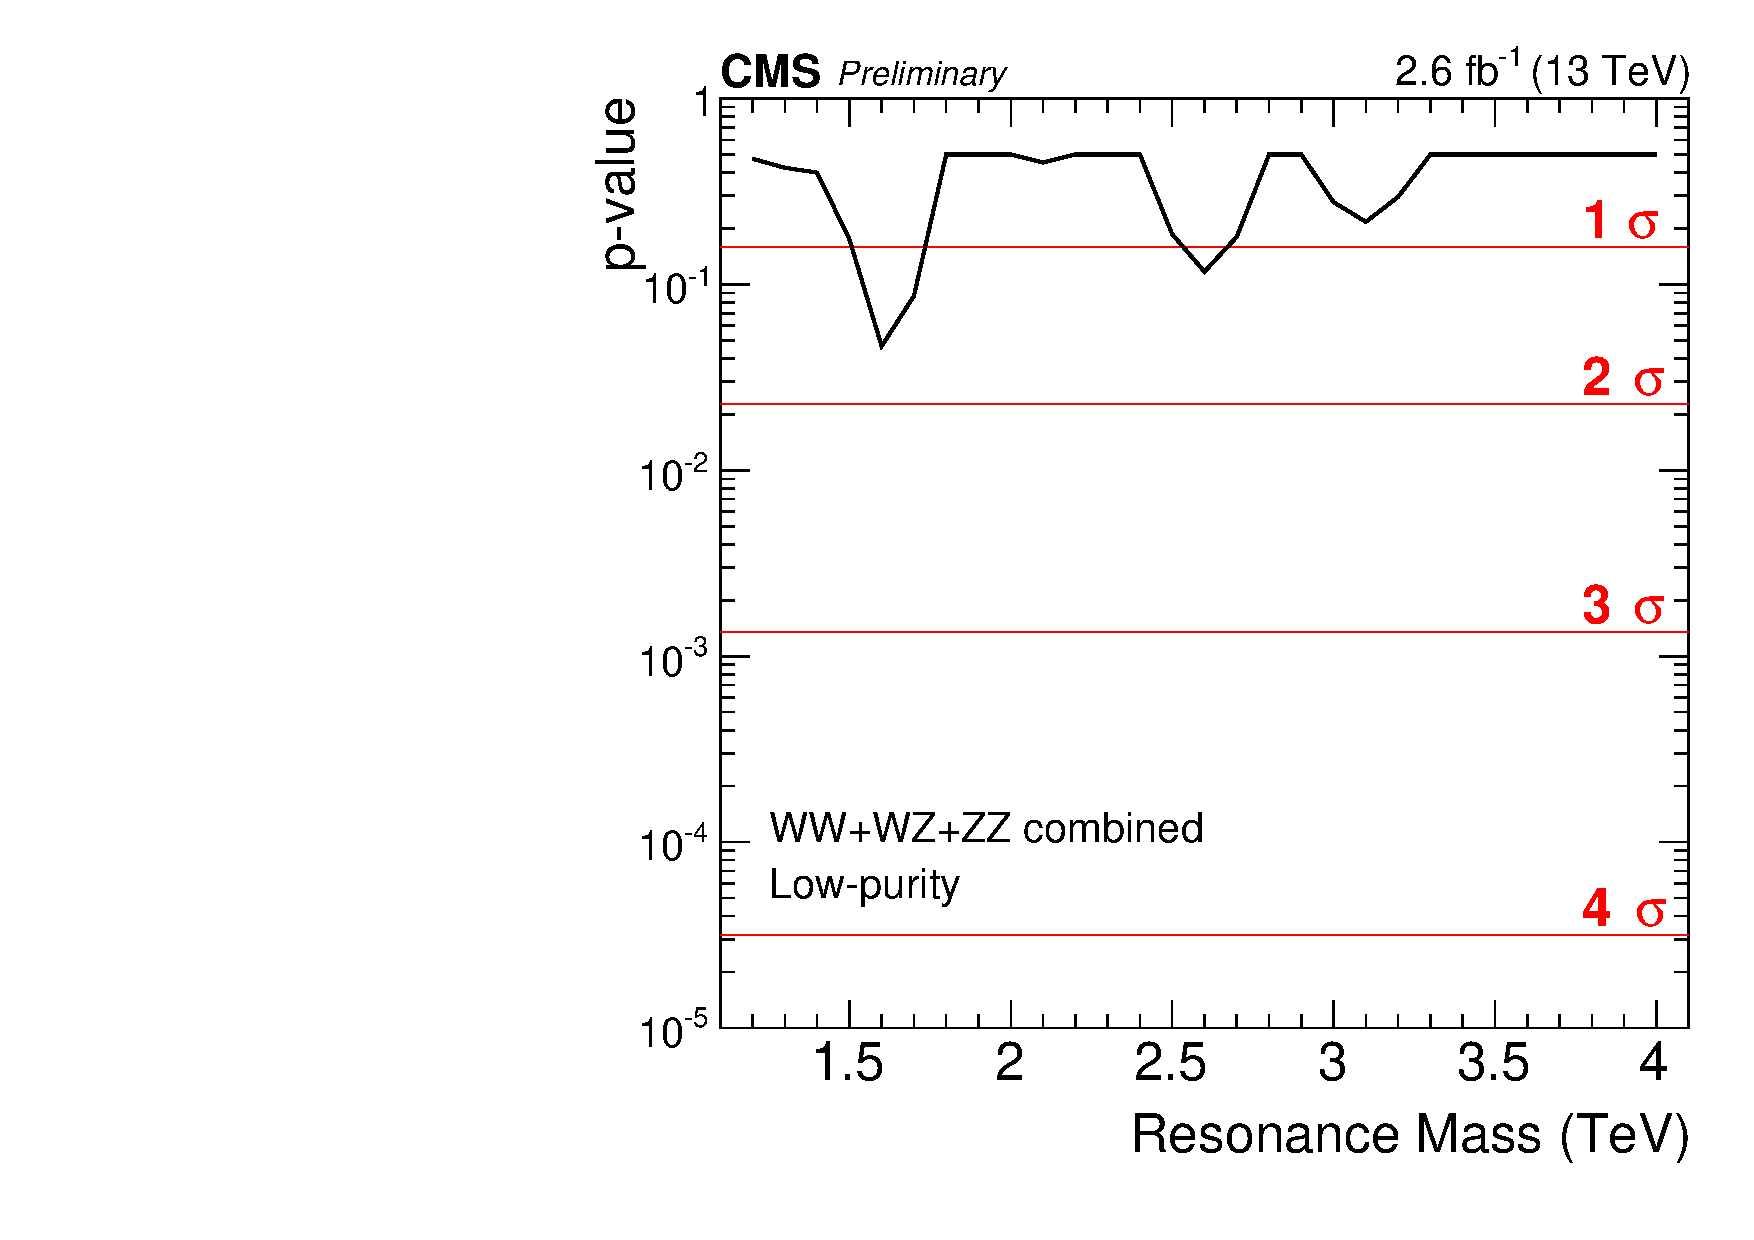
\includegraphics[width=0.32\textwidth]{figures/analysis/search1/AN-15-211/pvalues/pvalue_BulkZZinVVnew_low_purity.pdf}
\caption{Expected/observed limits and corresponding p-values obtained in the low purity category using 2.6 $\textrm{fb}^{-1}$ of CMS data. Here for a Bulk $G\rightarrow WW$ (left), $W'\rightarrow WZ$ (middle) and $G\rightarrow ZZ$ (right) signal.}
\label{fig:searchI:Limits_LP}
\end{figure}


\begin{figure}[h!]
\centering
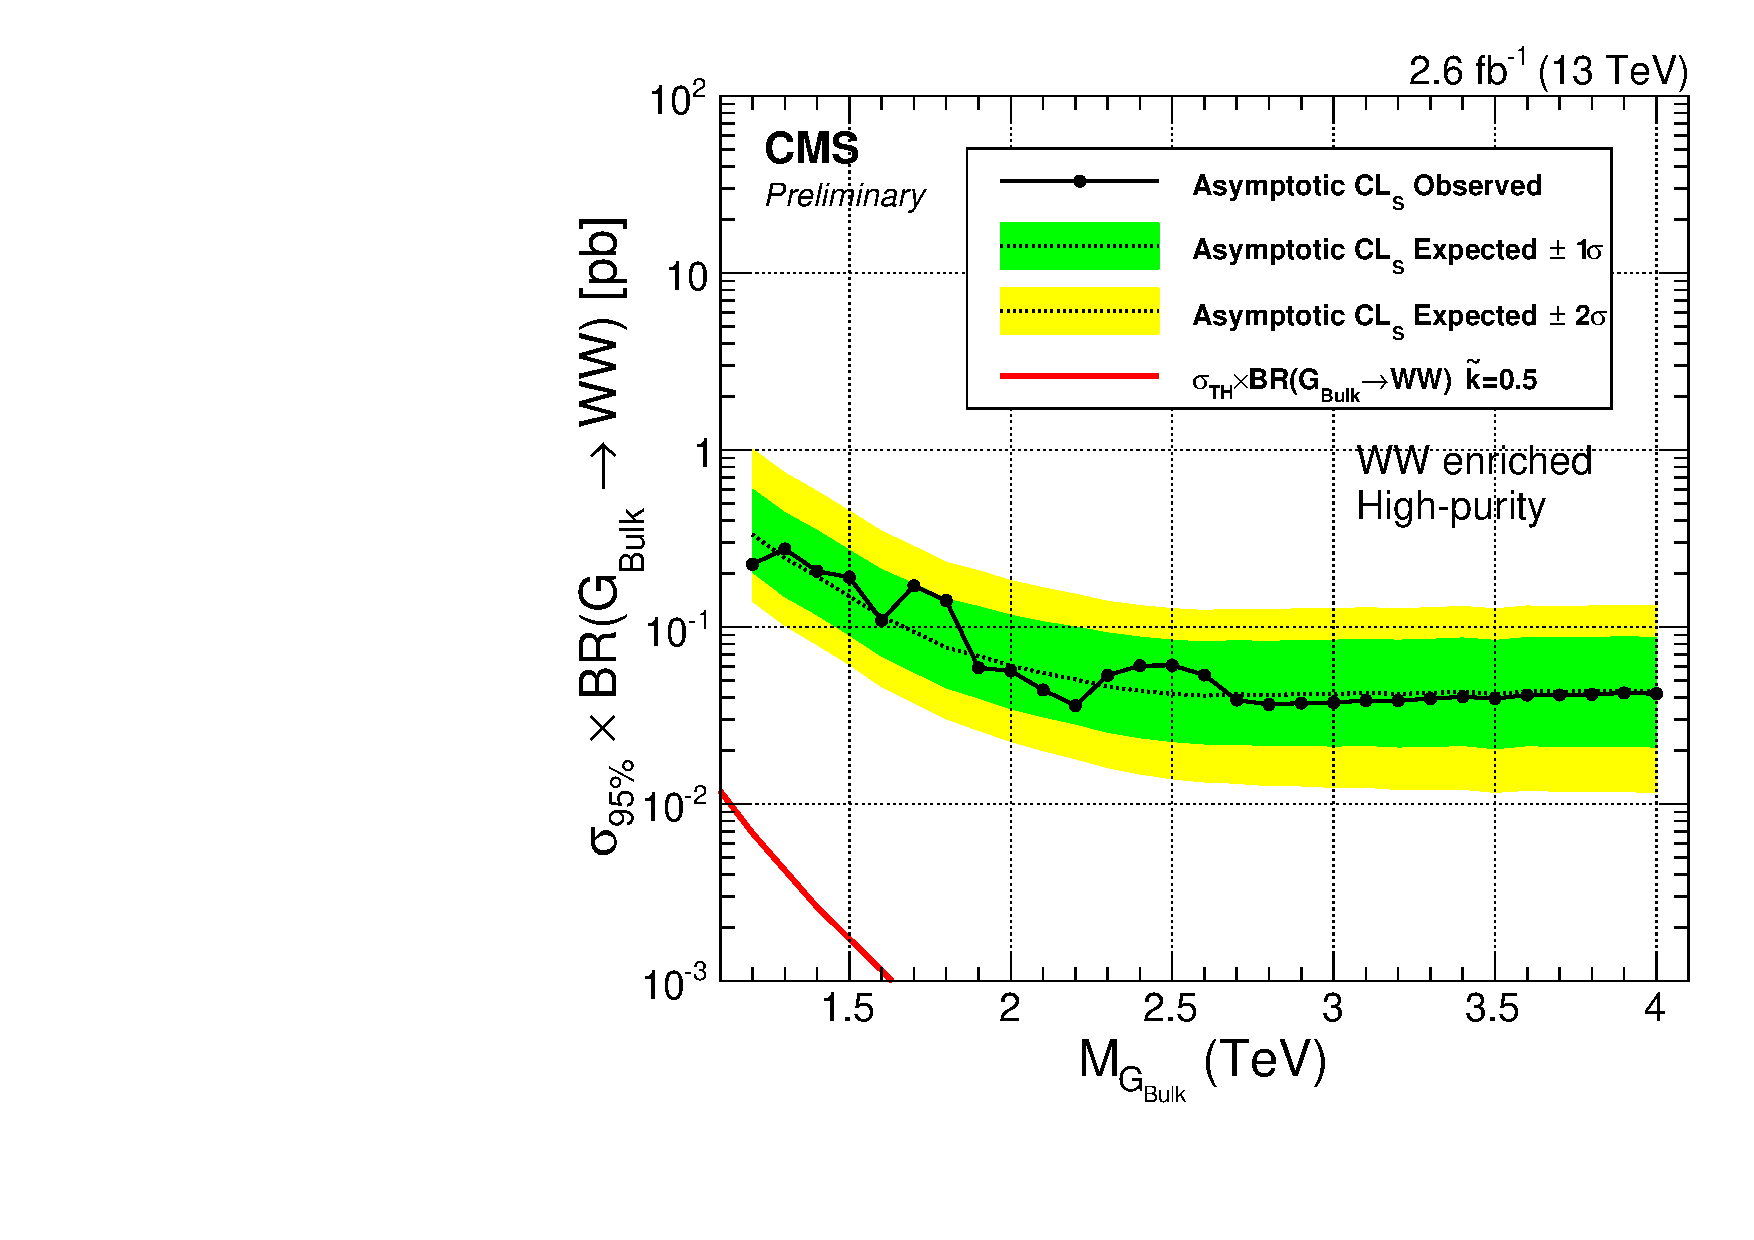
\includegraphics[width=0.32\textwidth]{figures/analysis/search1/AN-15-211/limits/brazilianFlag_BulkWW_WWHP_13TeV_wPDF.pdf}
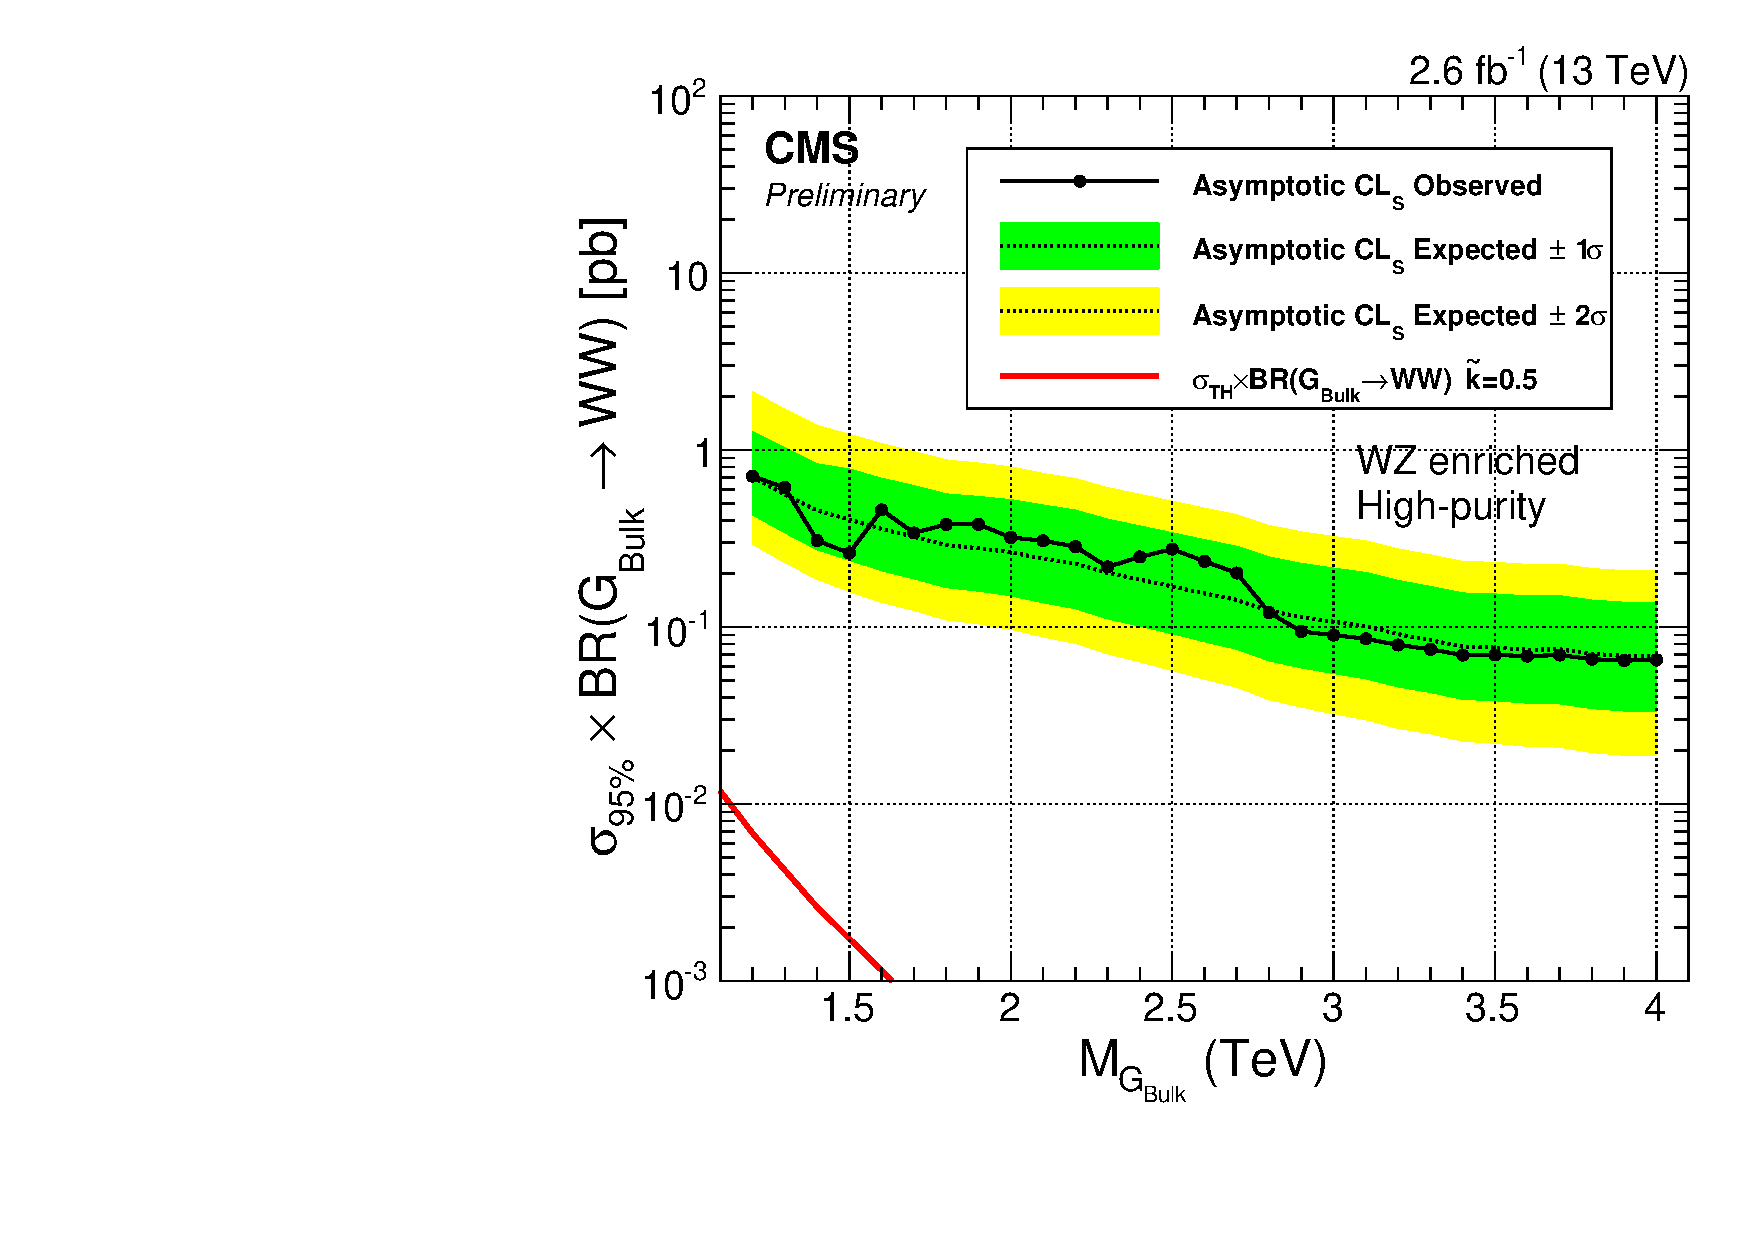
\includegraphics[width=0.32\textwidth]{figures/analysis/search1/AN-15-211/limits/brazilianFlag_BulkWW_WZHP_13TeV_wPDF.pdf}
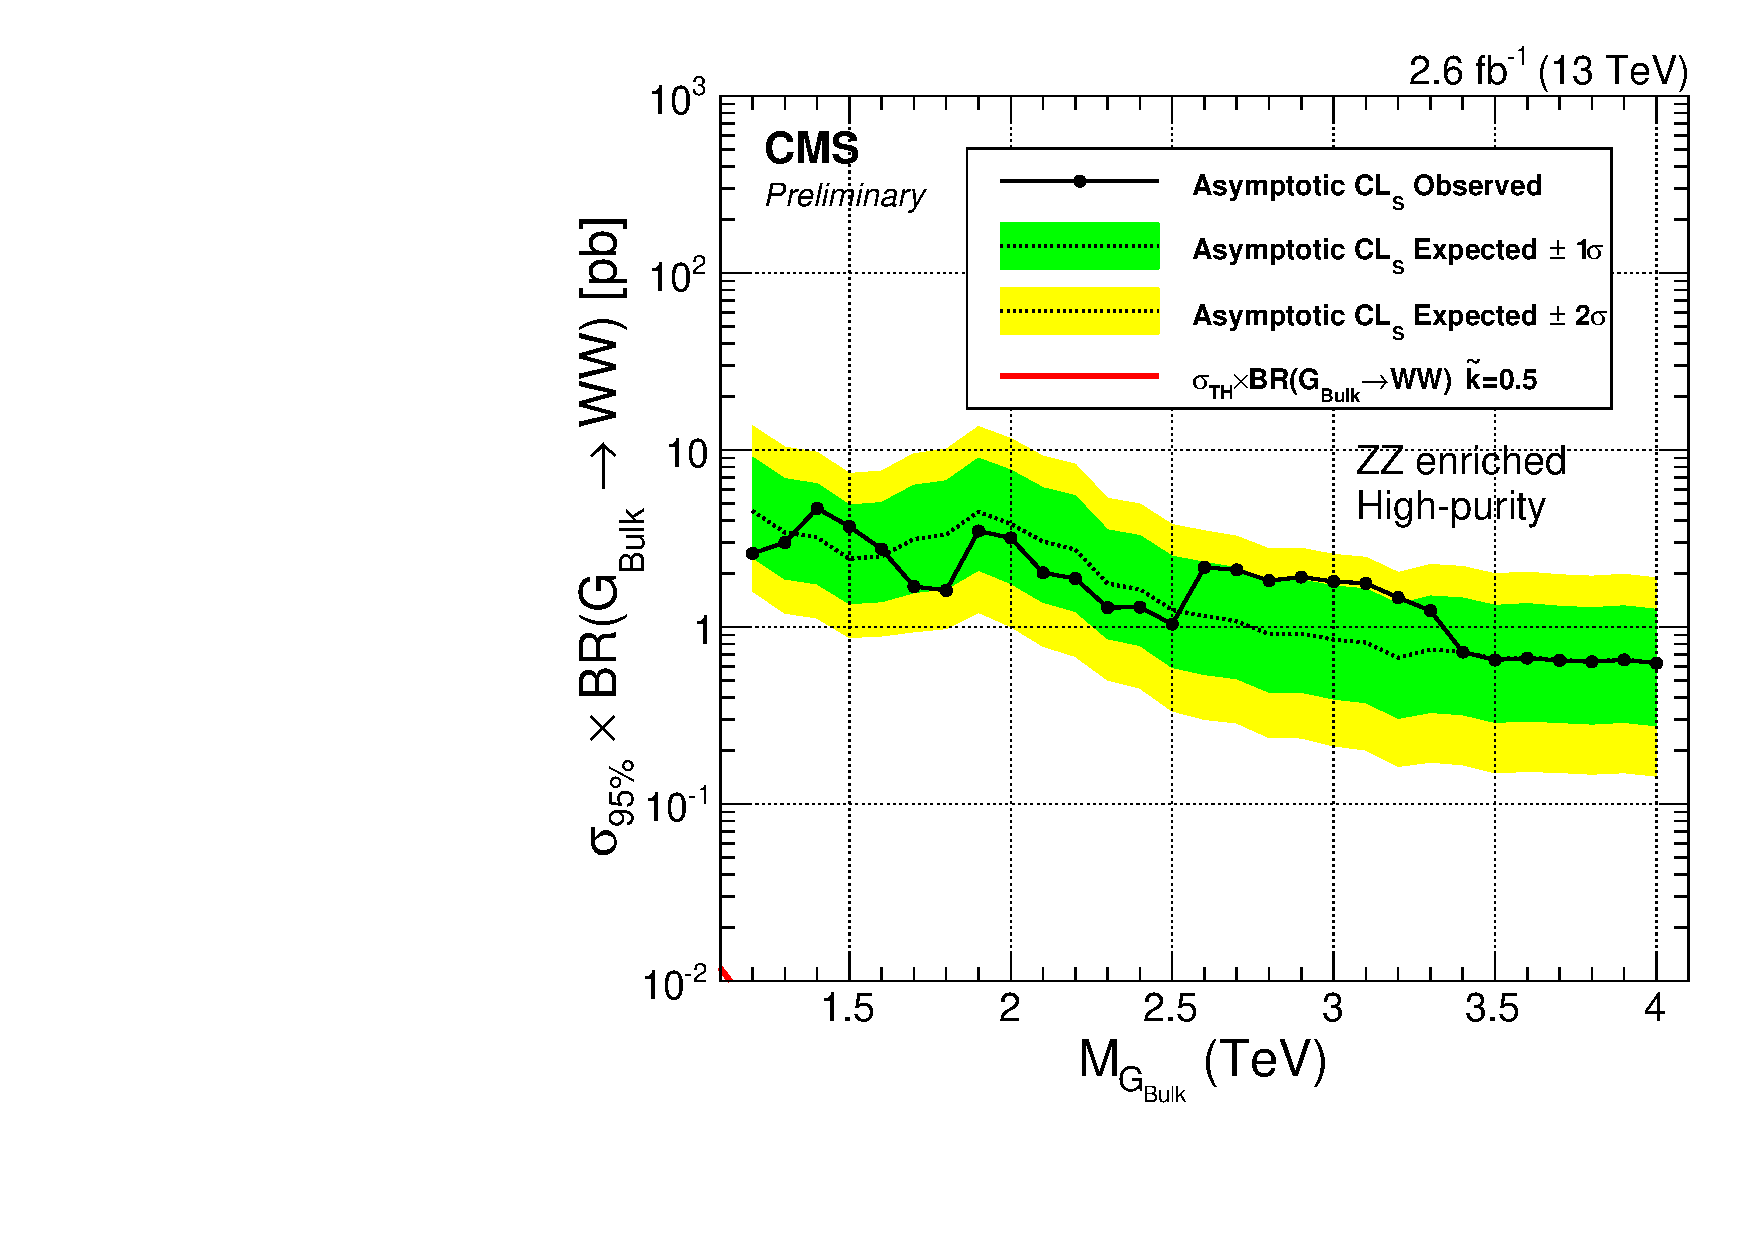
\includegraphics[width=0.32\textwidth]{figures/analysis/search1/AN-15-211/limits/brazilianFlag_BulkWW_ZZHP_13TeV_wPDF.pdf}\\
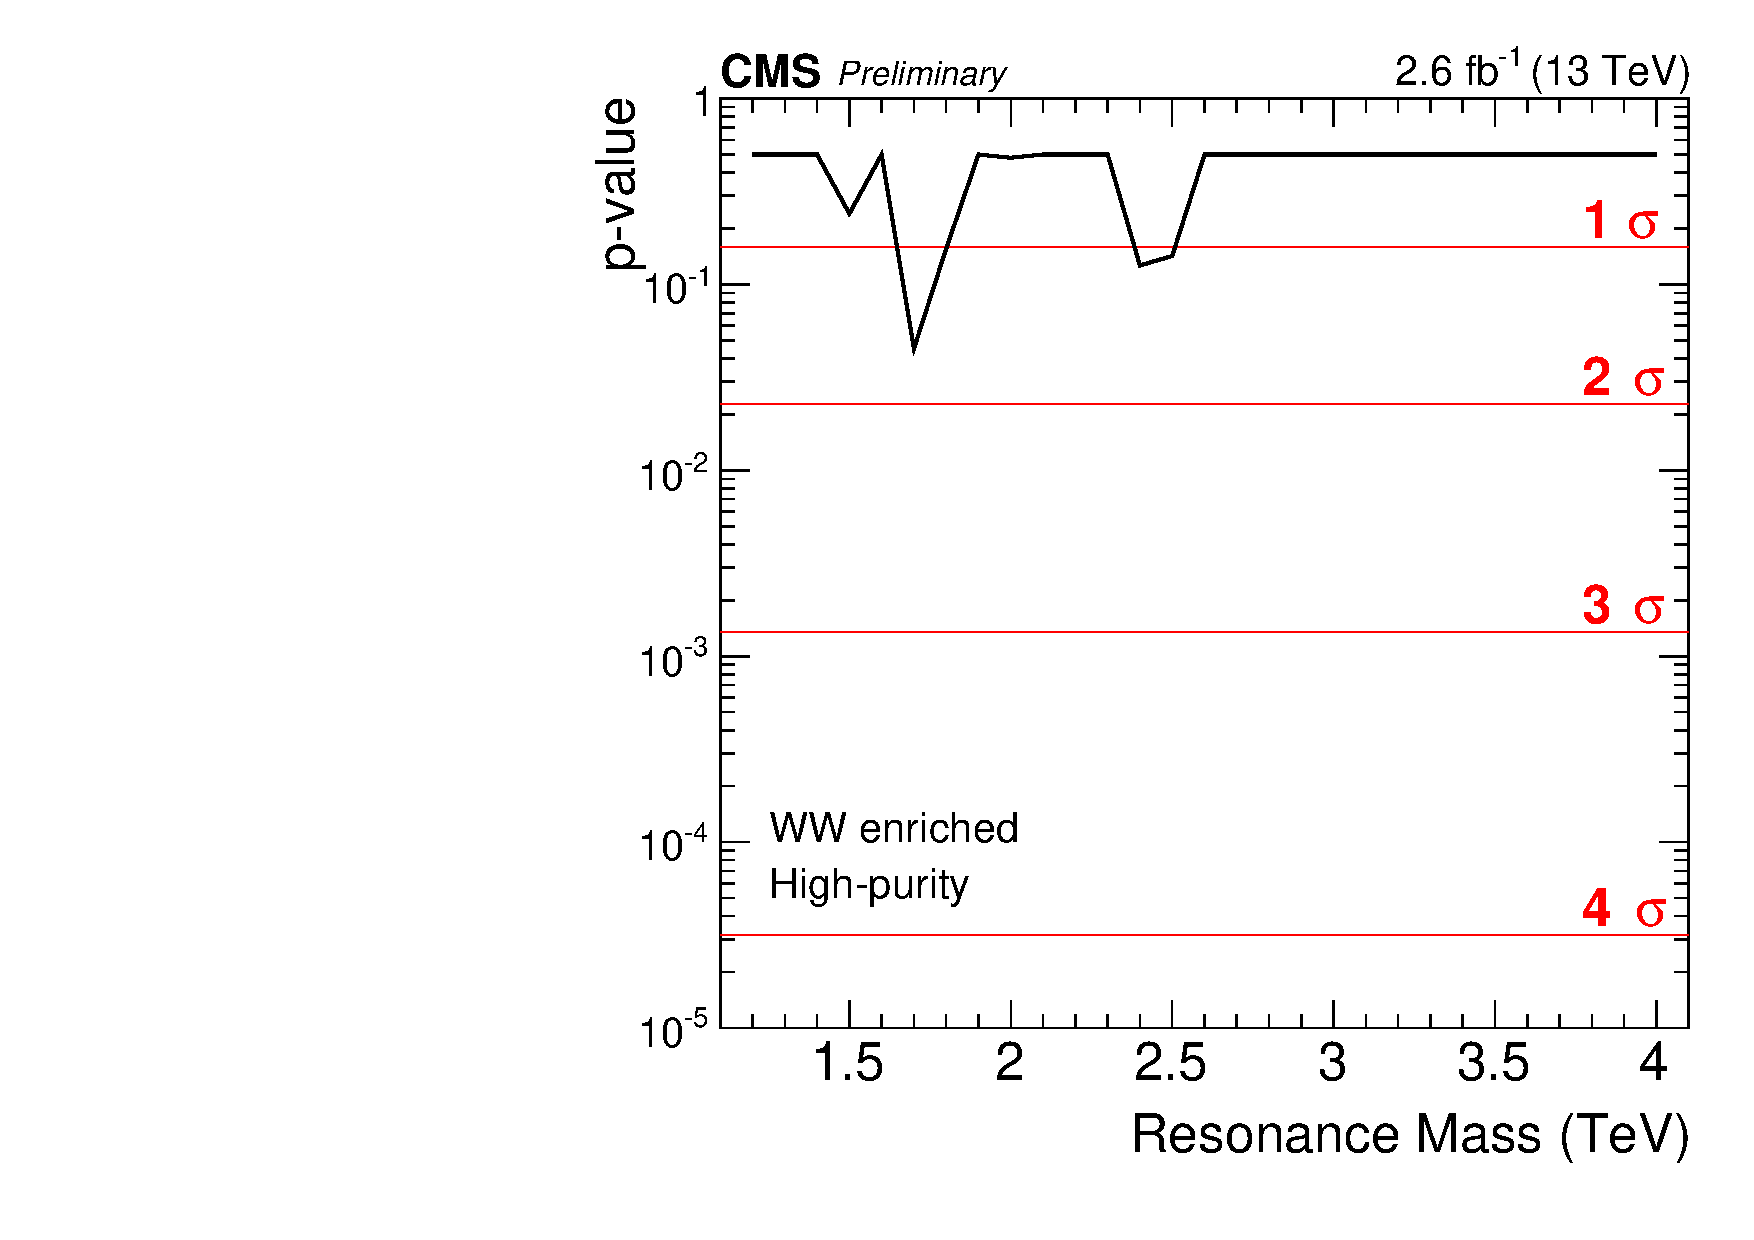
\includegraphics[width=0.32\textwidth]{figures/analysis/search1/AN-15-211/pvalues/pvalue_BulkWWinWW_high_purity.pdf}
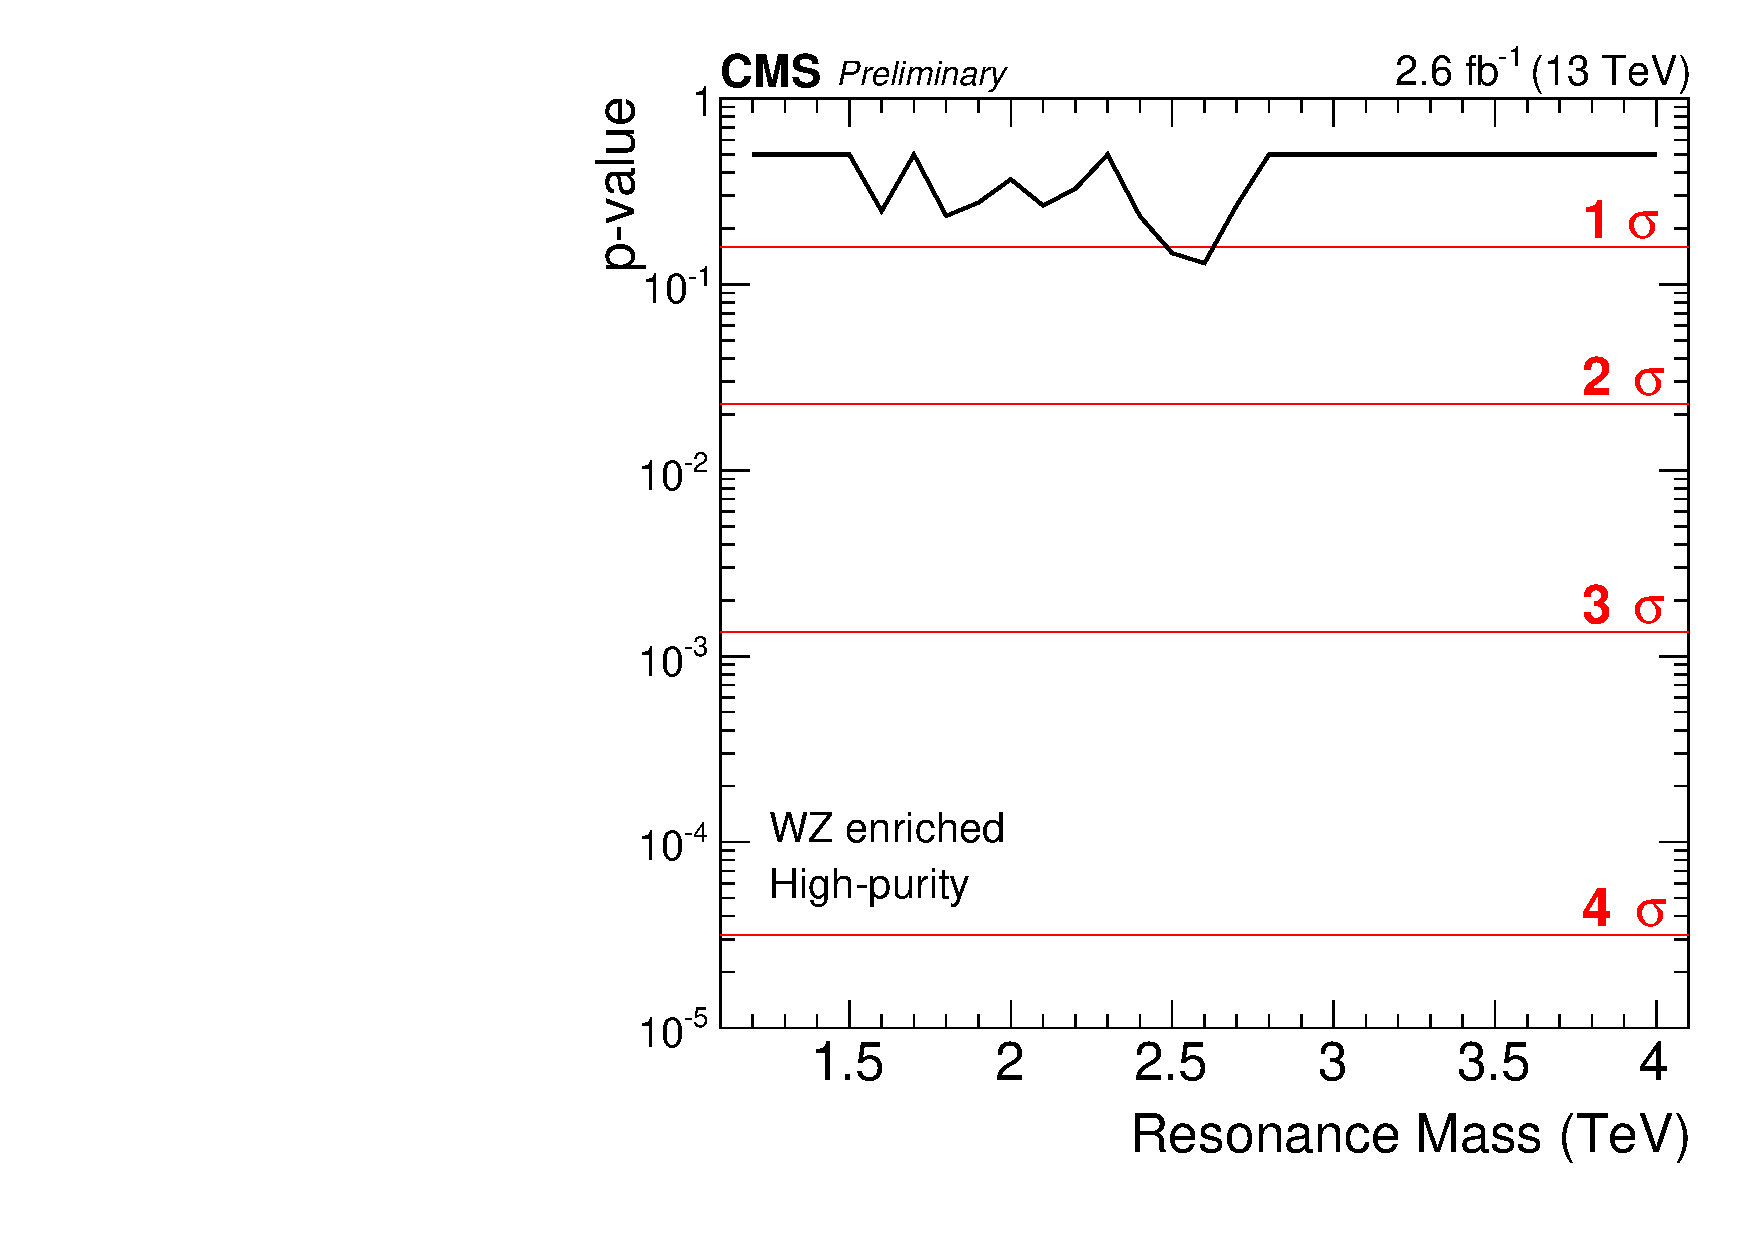
\includegraphics[width=0.32\textwidth]{figures/analysis/search1/AN-15-211/pvalues/pvalue_BulkWWinWZ_high_purity.pdf}
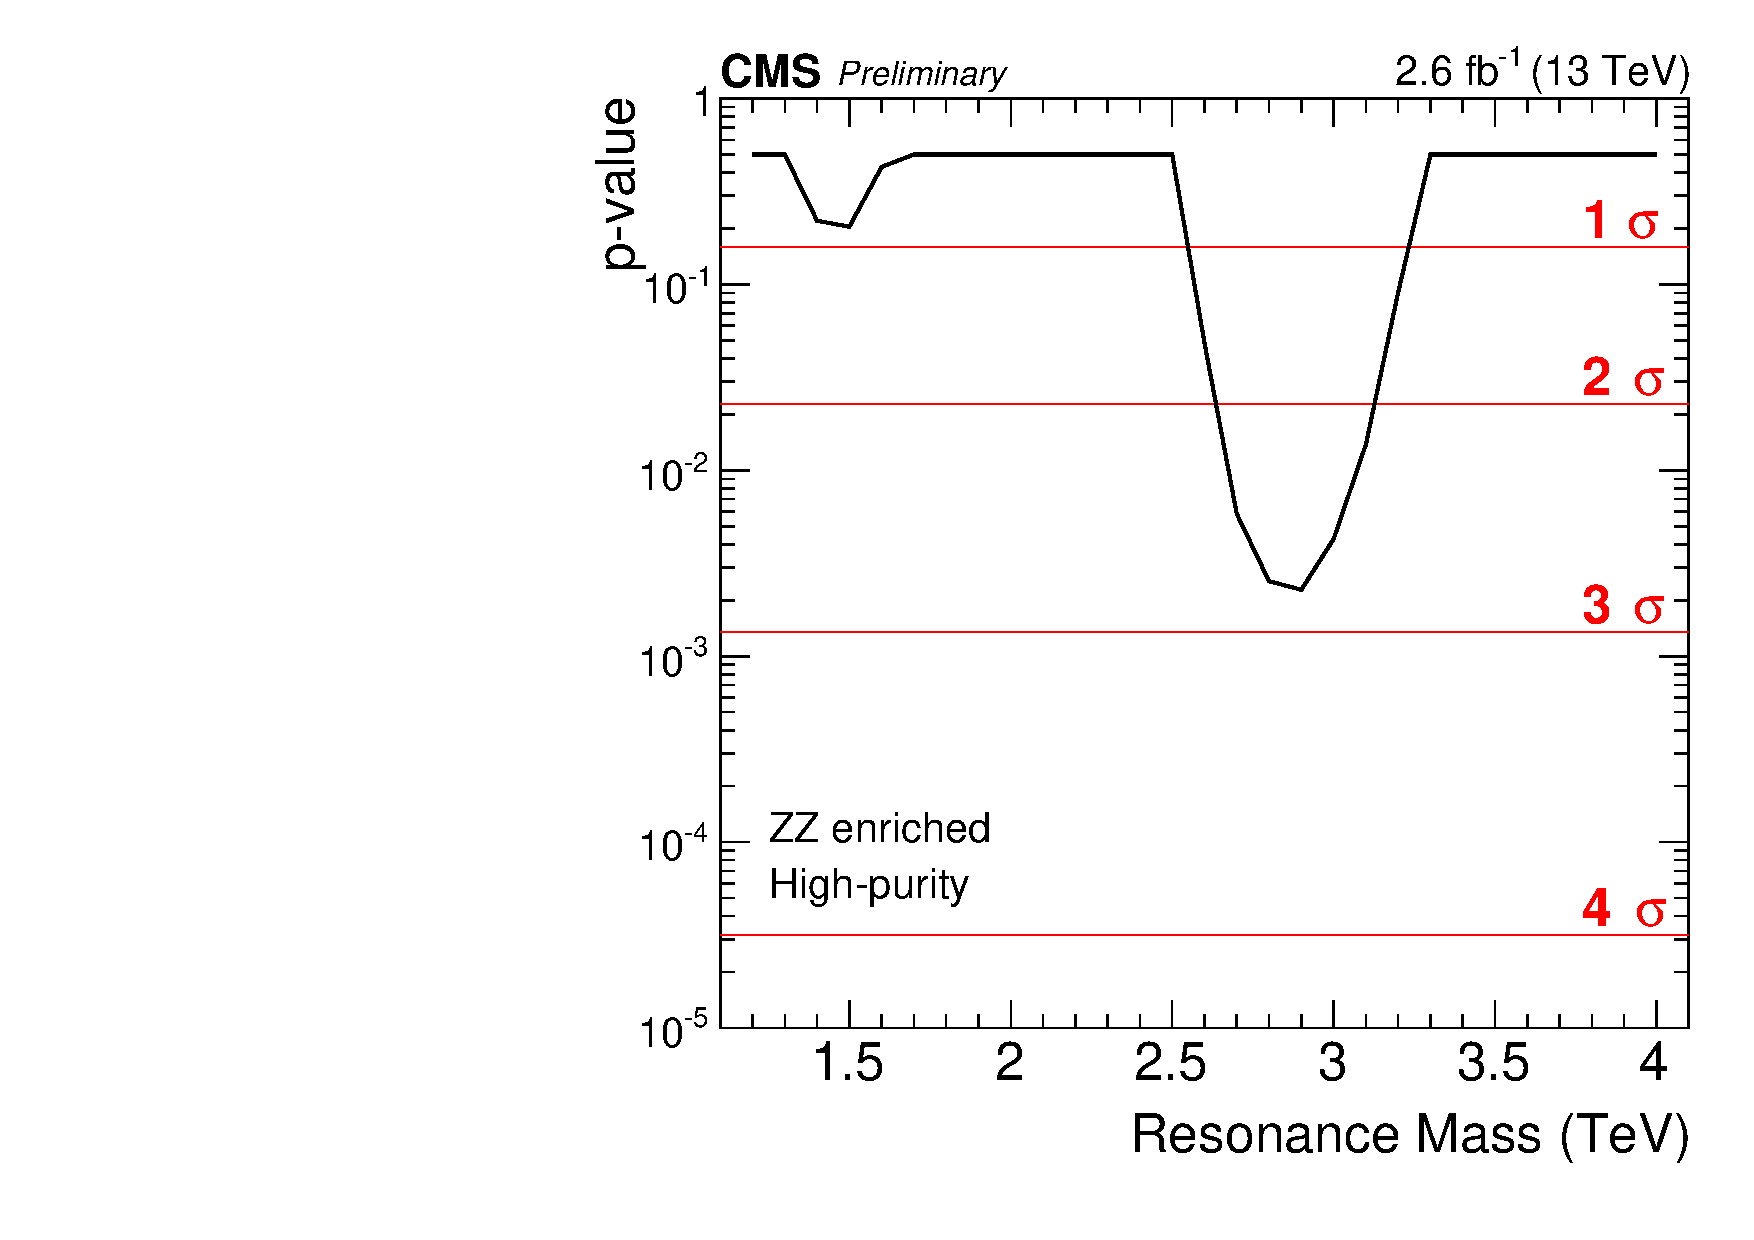
\includegraphics[width=0.32\textwidth]{figures/analysis/search1/AN-15-211/pvalues/pvalue_BulkWWinZZ_high_purity.pdf}
\caption{Expected/observed limits and corresponding p-values obtained for the different mass categories using 2.6 $\textrm{fb}^{-1}$ of CMS data. Here for a Bulk $G\rightarrow WW$ signal in the HP category}
\label{fig:searchI:Limits_HPBulkWW}
\end{figure}


\begin{figure}[h!]
\centering
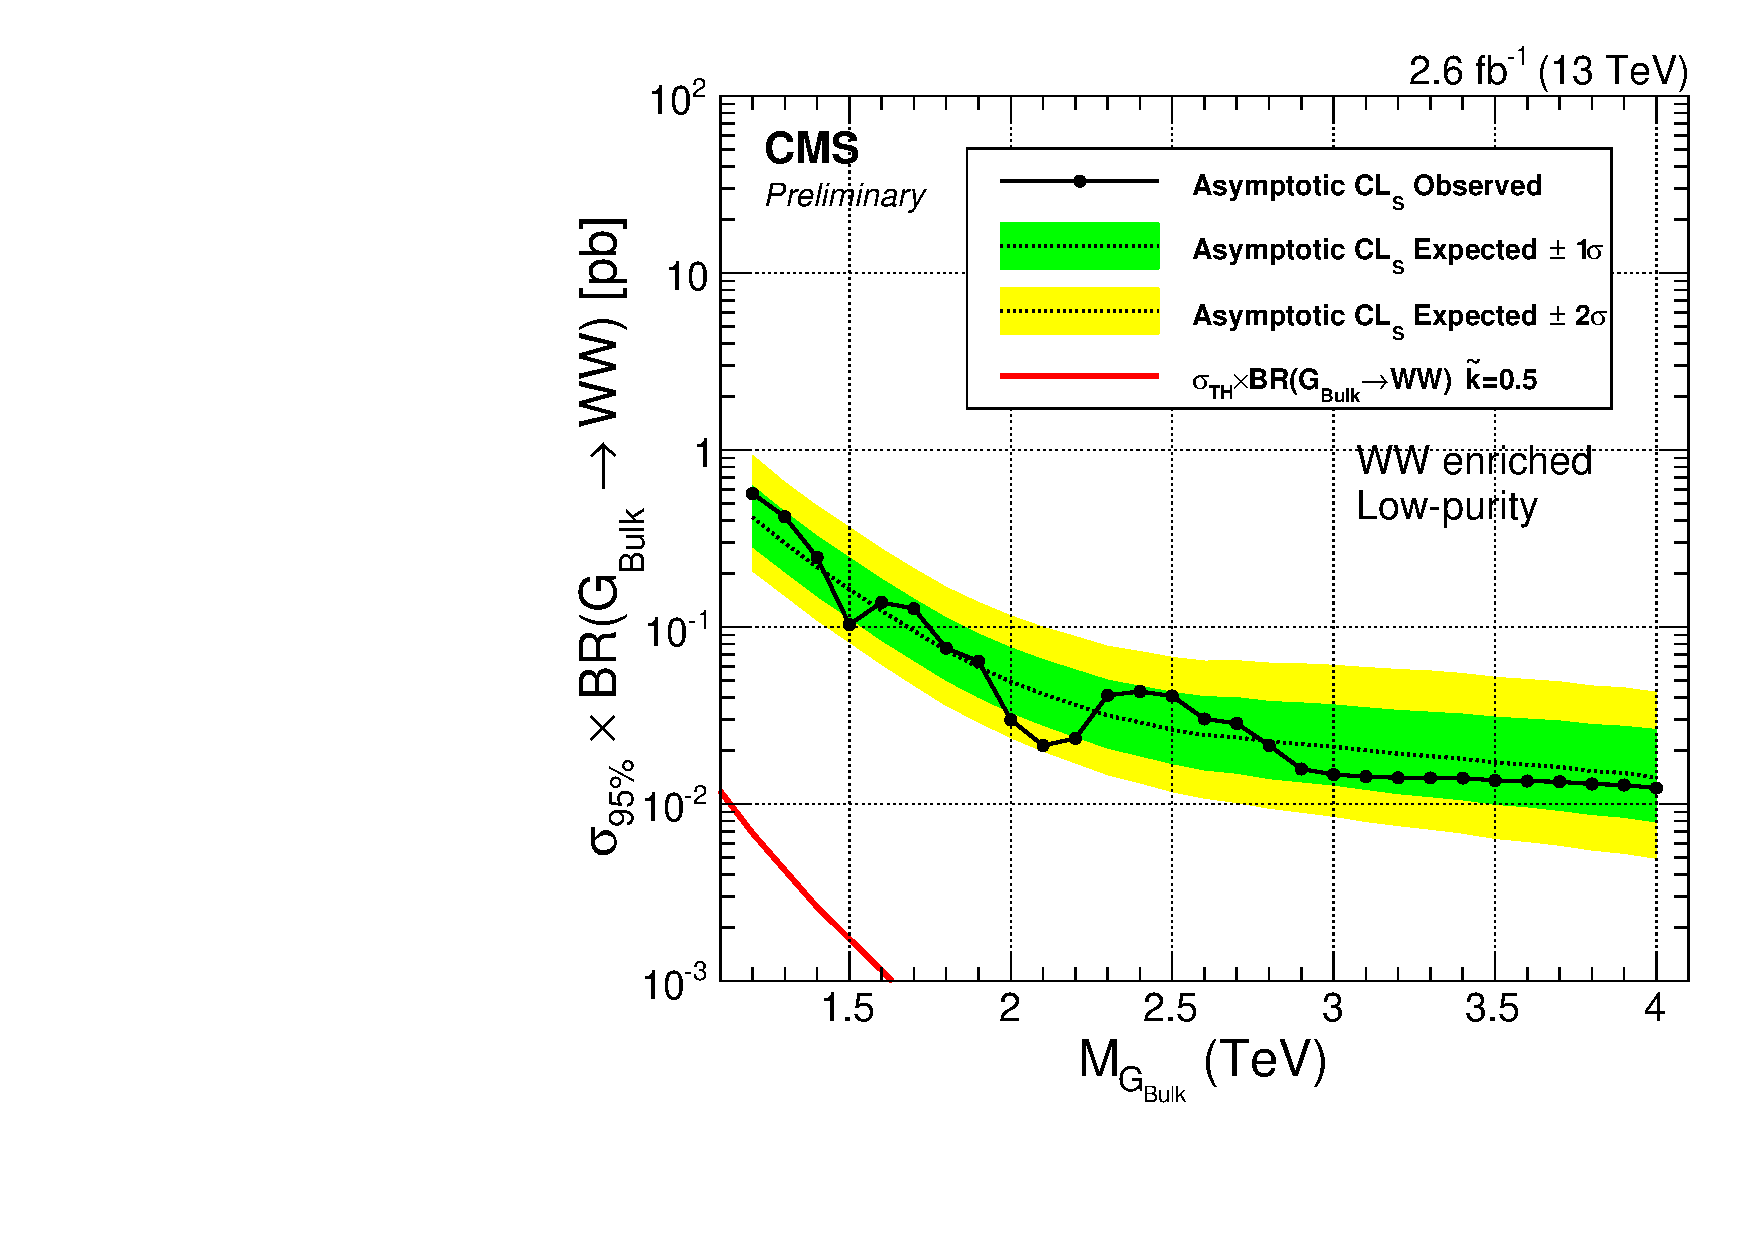
\includegraphics[width=0.32\textwidth]{figures/analysis/search1/AN-15-211/limits/brazilianFlag_BulkWW_WWLP_13TeV_wPDF.pdf}
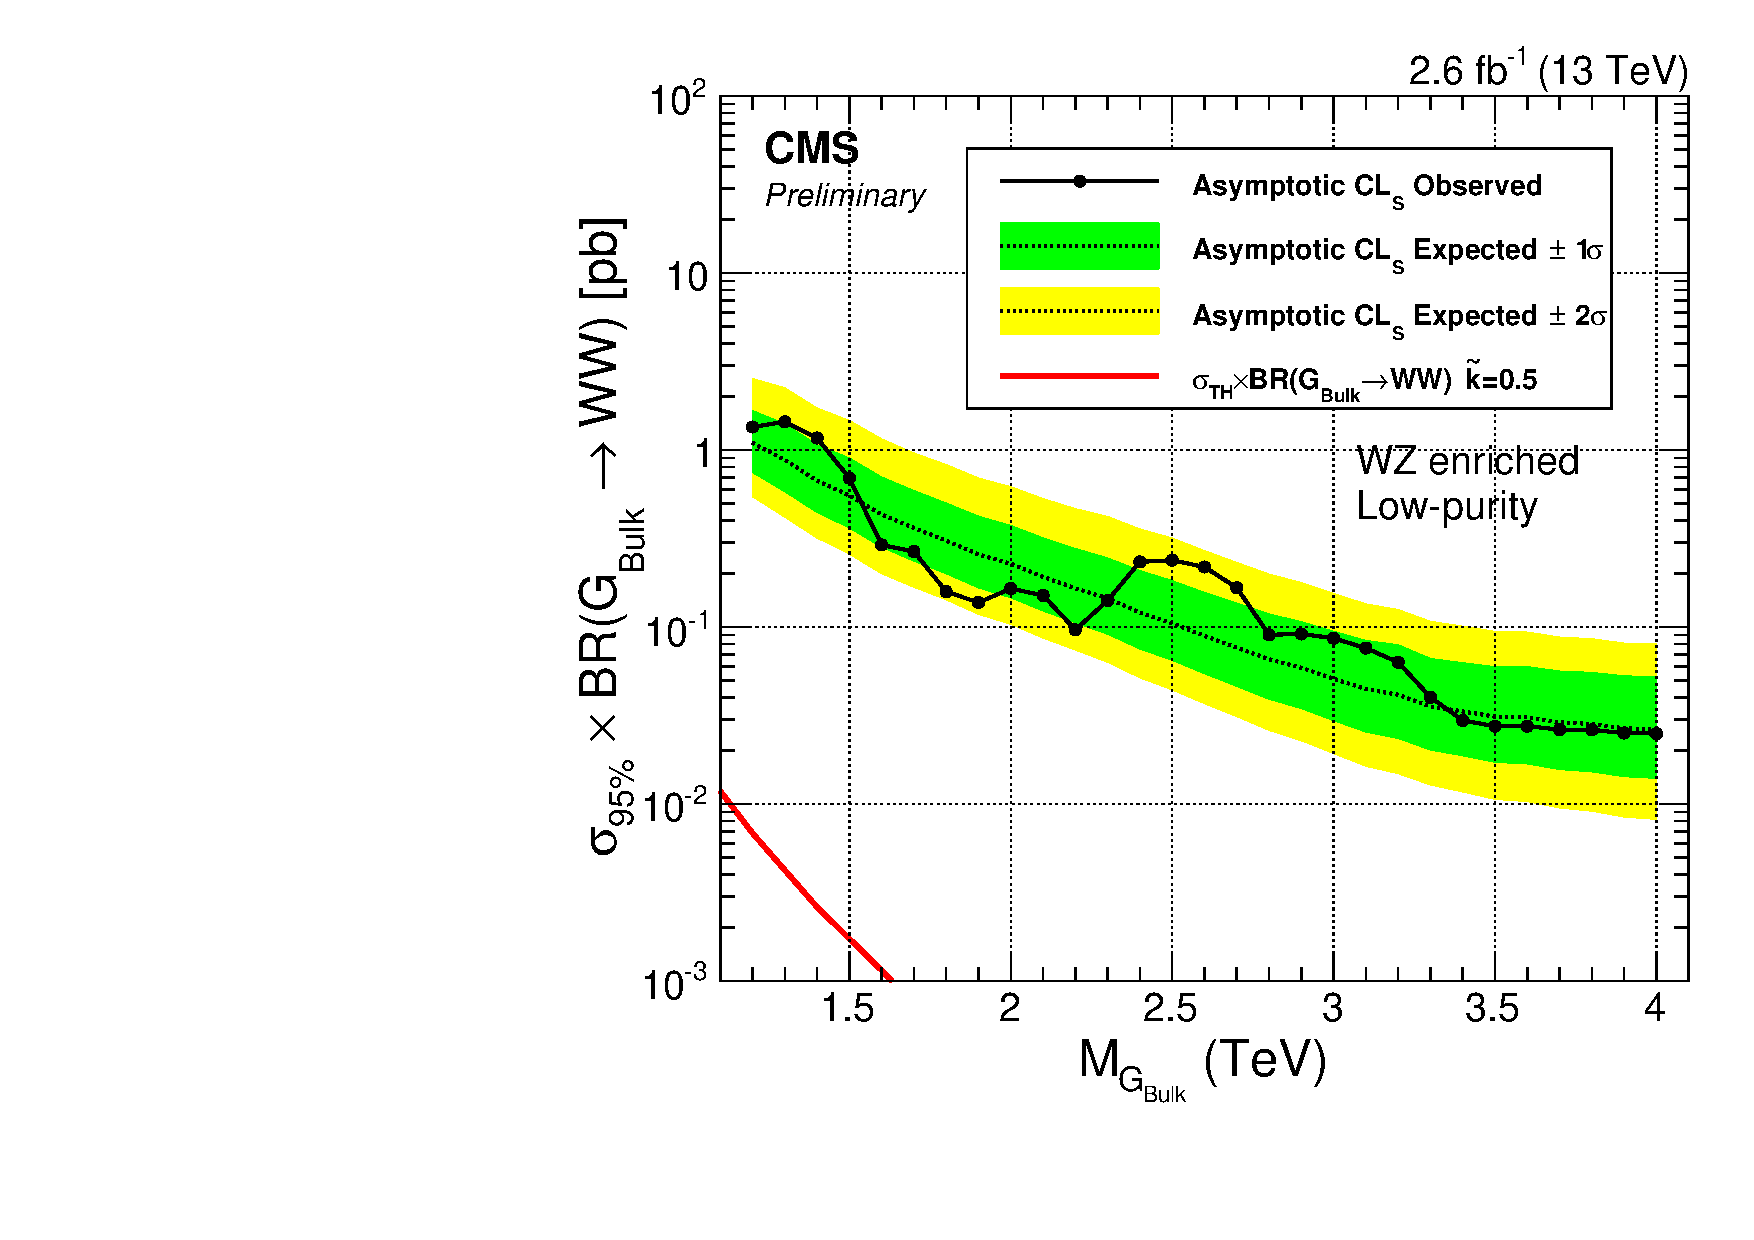
\includegraphics[width=0.32\textwidth]{figures/analysis/search1/AN-15-211/limits/brazilianFlag_BulkWW_WZLP_13TeV_wPDF.pdf}
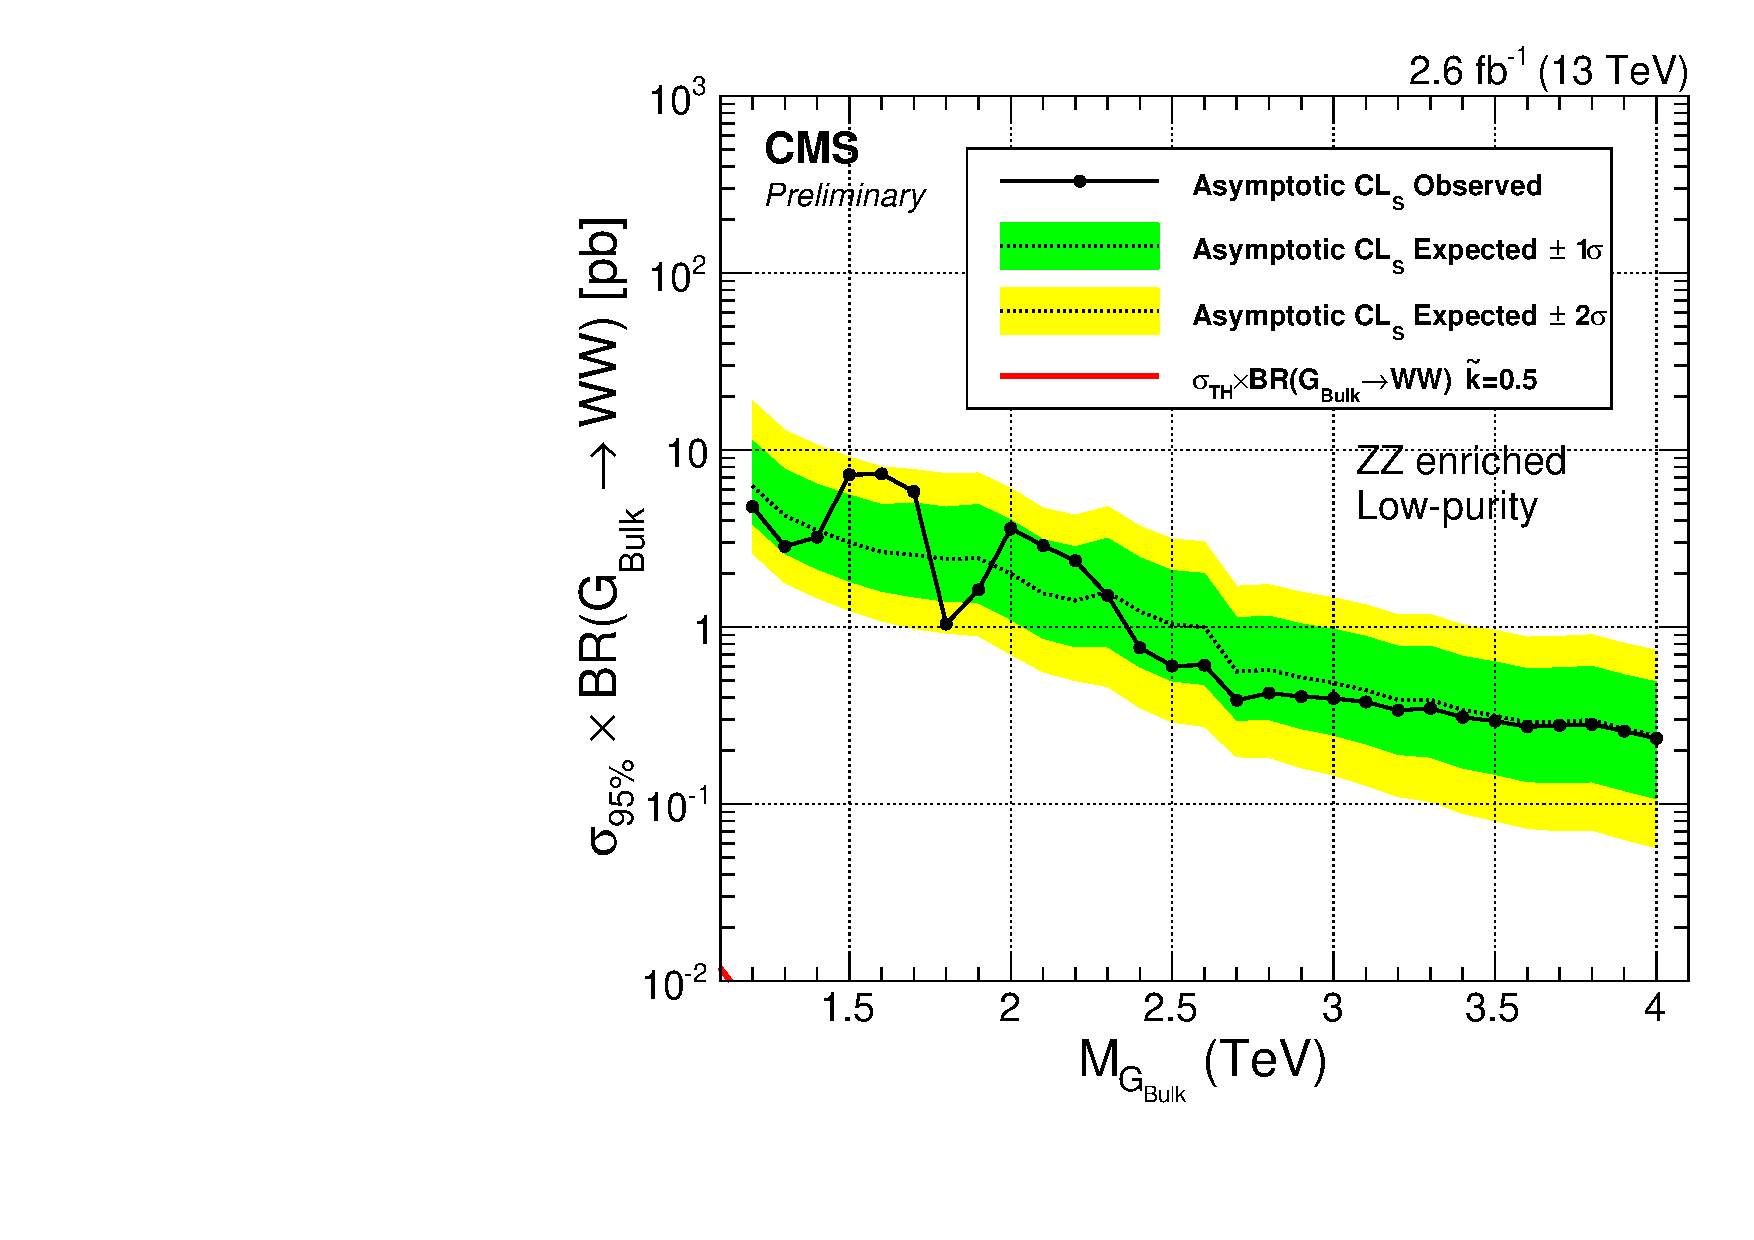
\includegraphics[width=0.32\textwidth]{figures/analysis/search1/AN-15-211/limits/brazilianFlag_BulkWW_ZZLP_13TeV_wPDF.pdf}\\
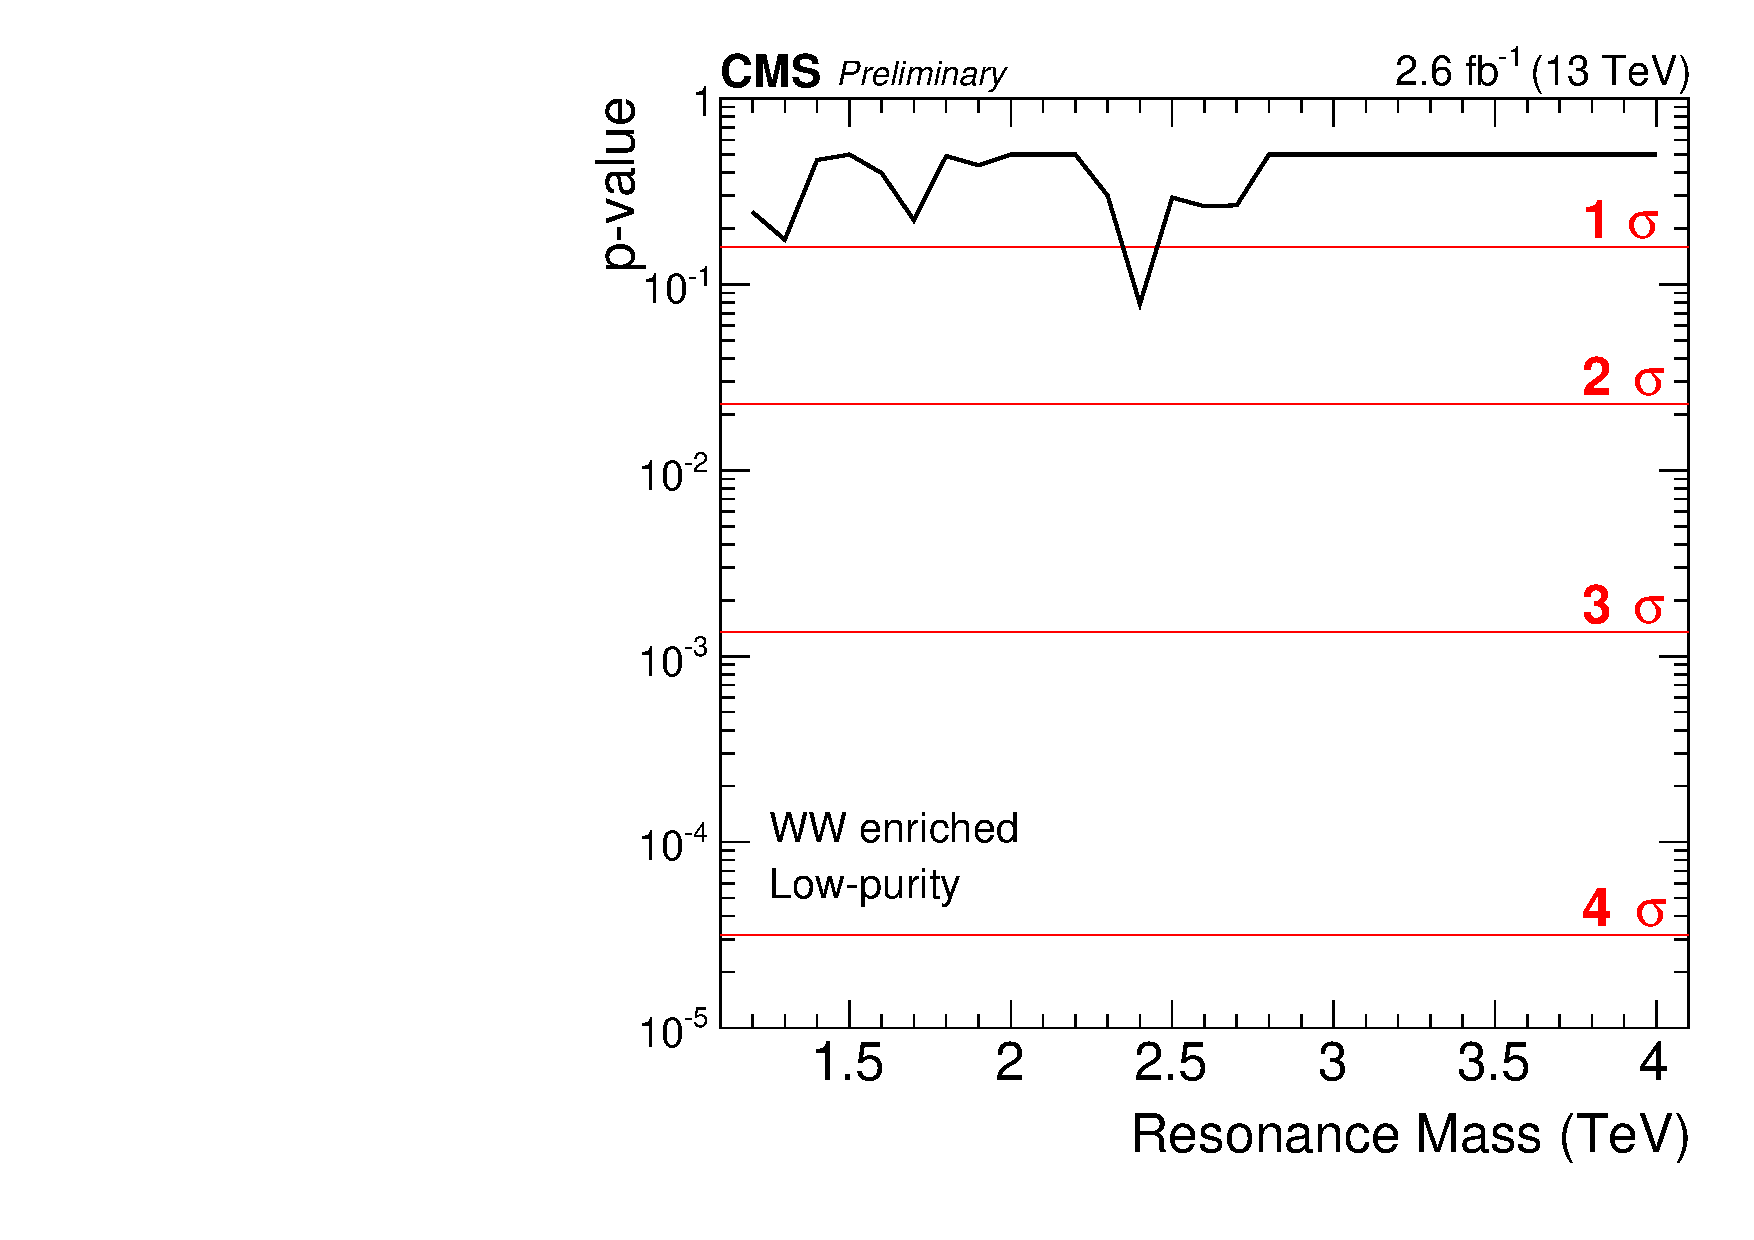
\includegraphics[width=0.32\textwidth]{figures/analysis/search1/AN-15-211/pvalues/pvalue_BulkWWinWW_low_purity.pdf}
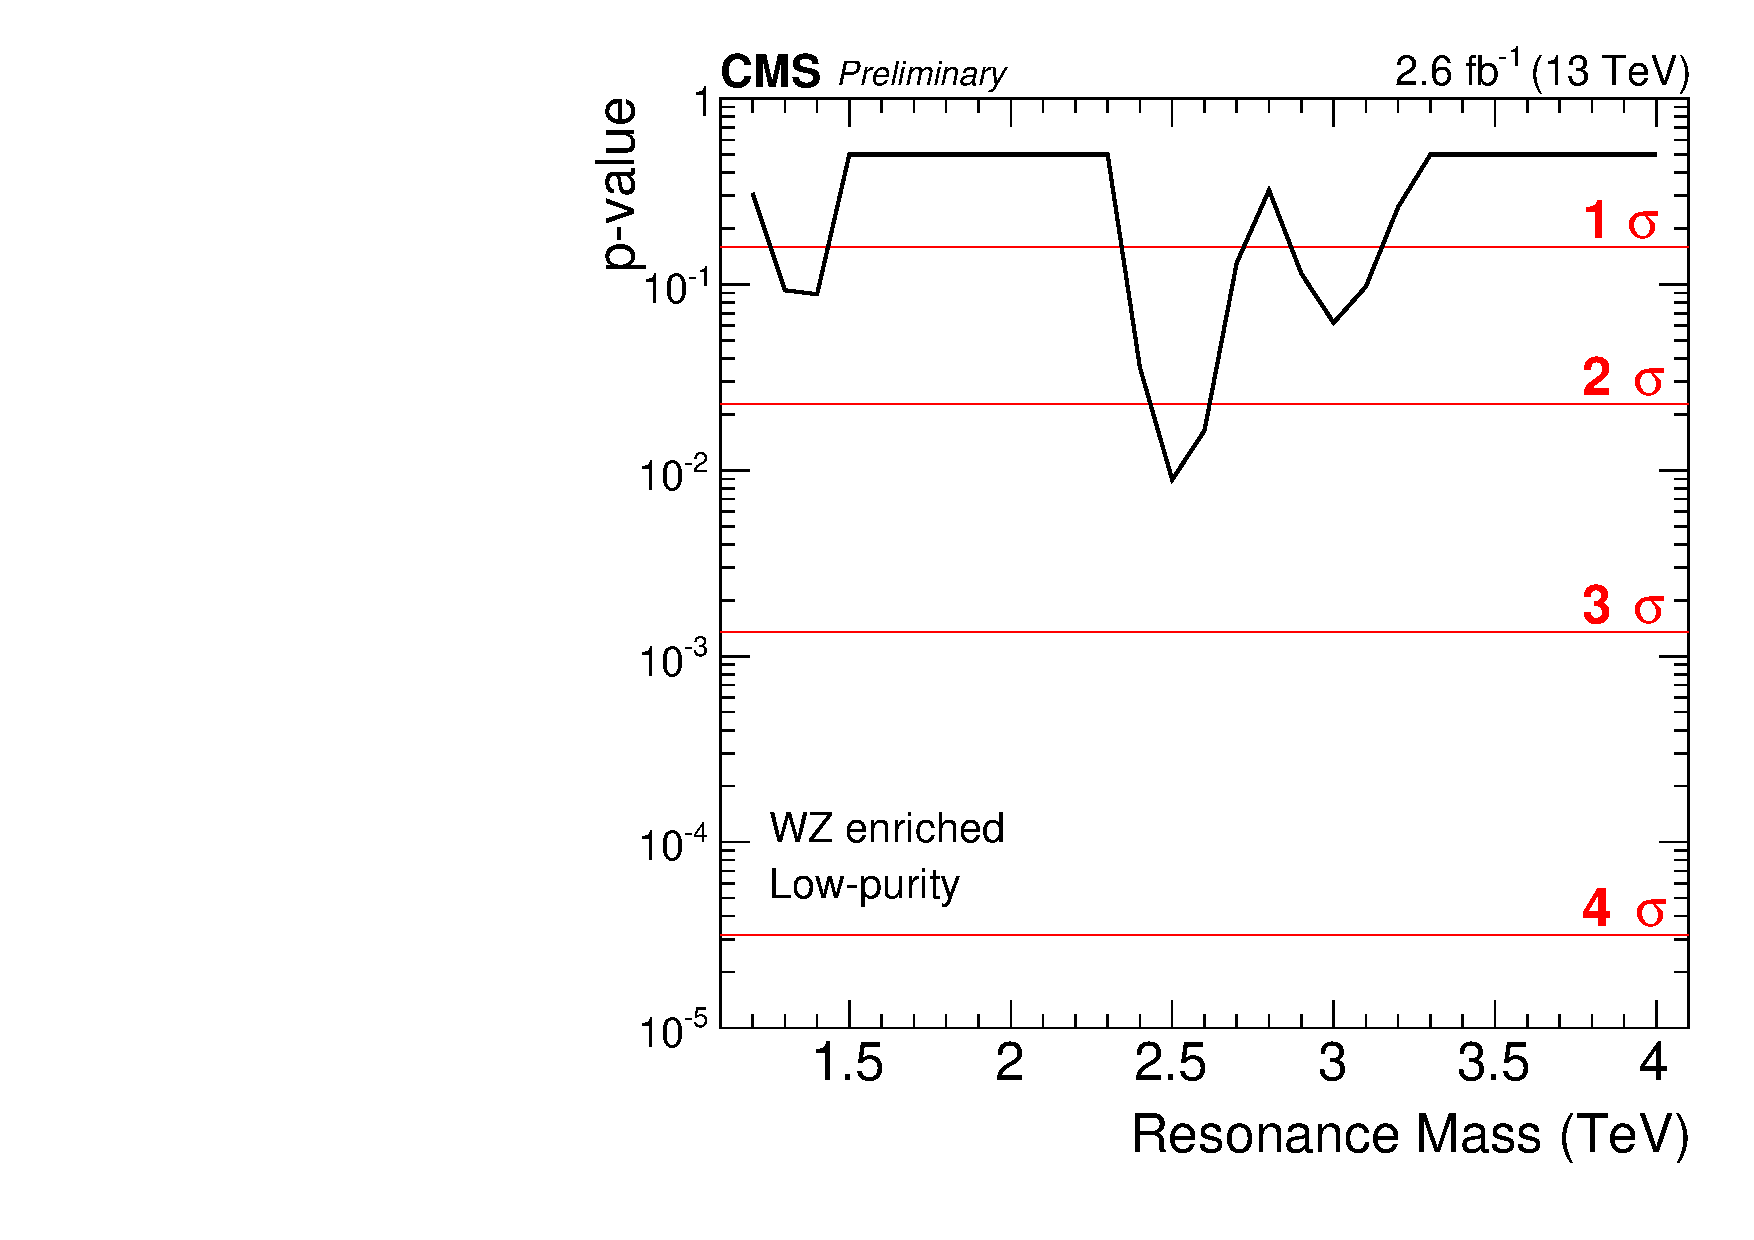
\includegraphics[width=0.32\textwidth]{figures/analysis/search1/AN-15-211/pvalues/pvalue_BulkWWinWZ_low_purity.pdf}
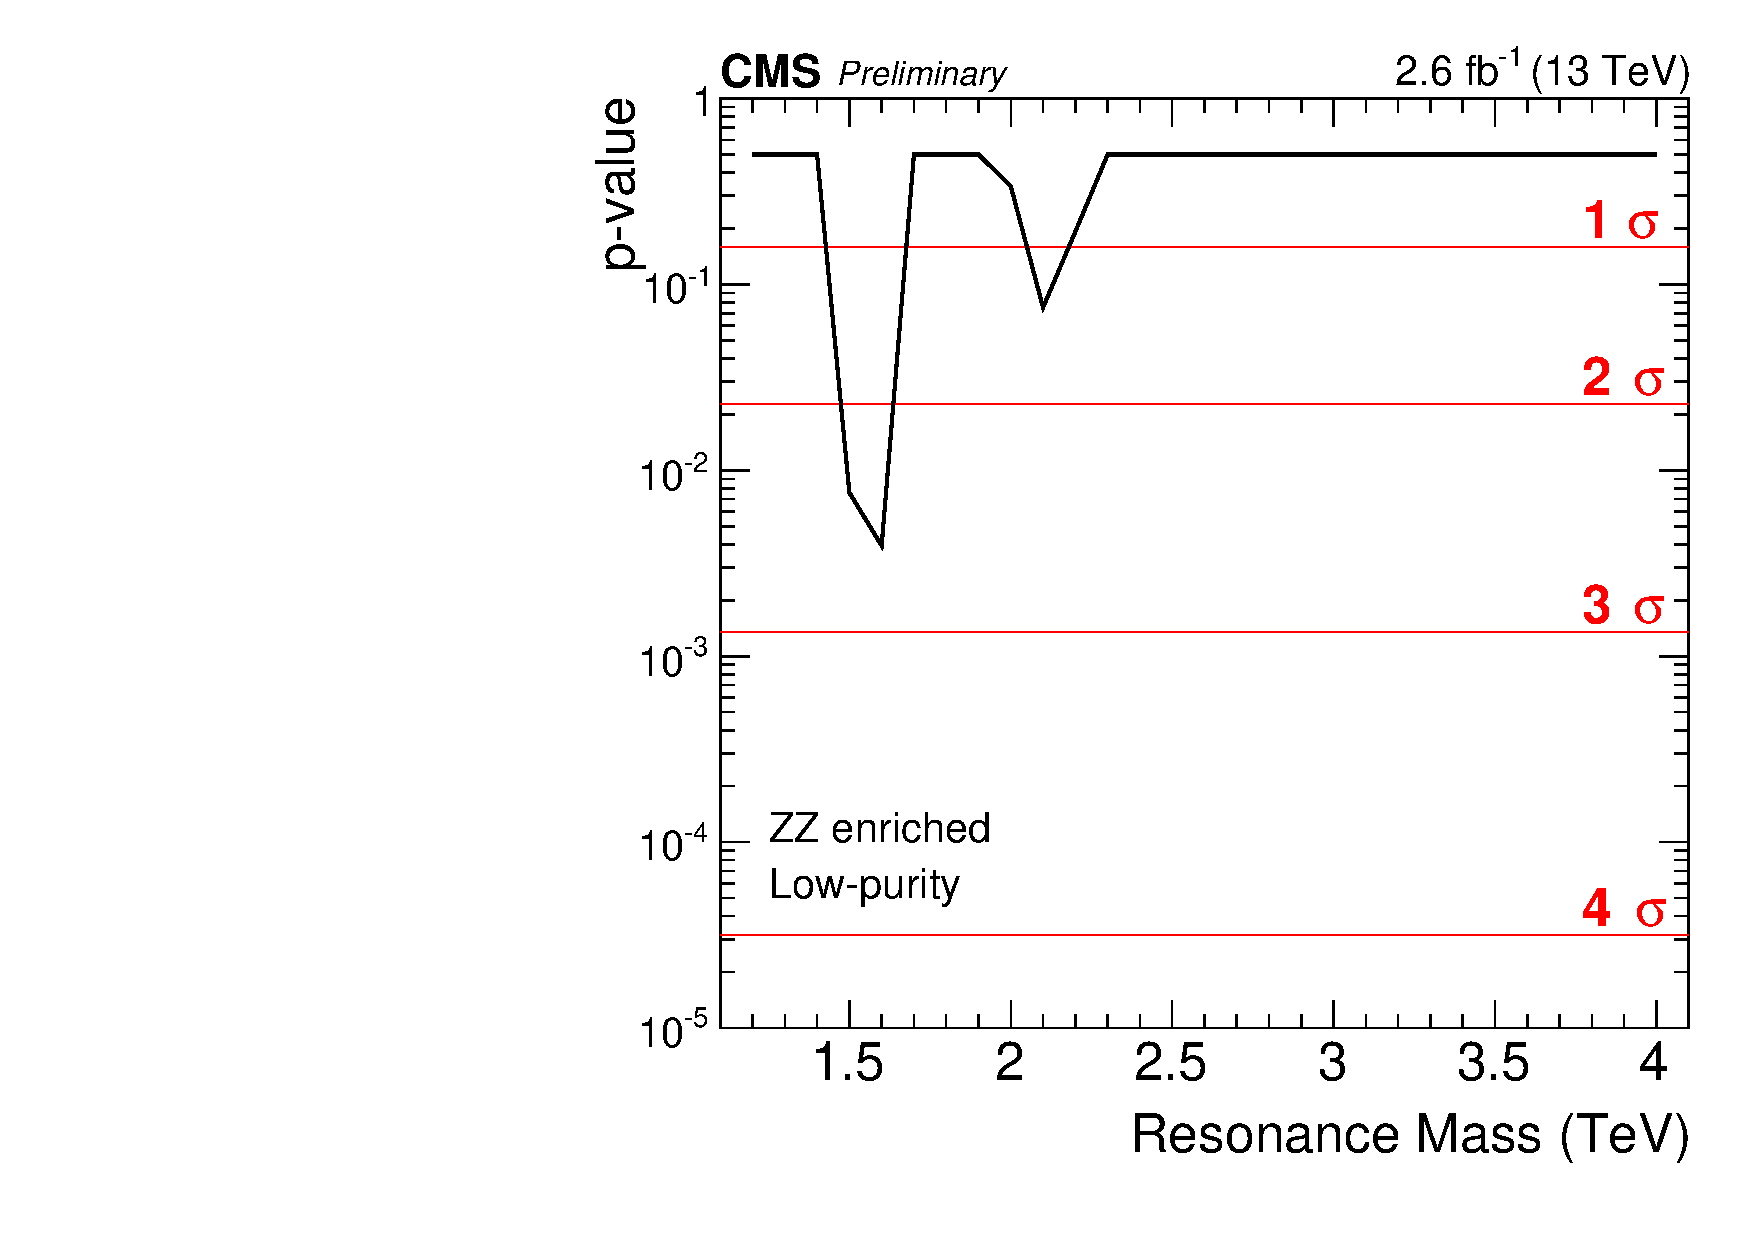
\includegraphics[width=0.32\textwidth]{figures/analysis/search1/AN-15-211/pvalues/pvalue_BulkWWinZZ_low_purity.pdf}
\caption{Expected/observed limits and corresponding p-values obtained in the different mass categories using 2.6 $\textrm{fb}^{-1}$ of CMS data. Here for a Bulk $G\rightarrow WW$ signal in the LP category.}
\label{fig:searchI:Limits_LPBulkWW}
\end{figure}



\begin{figure}[h!]
\centering
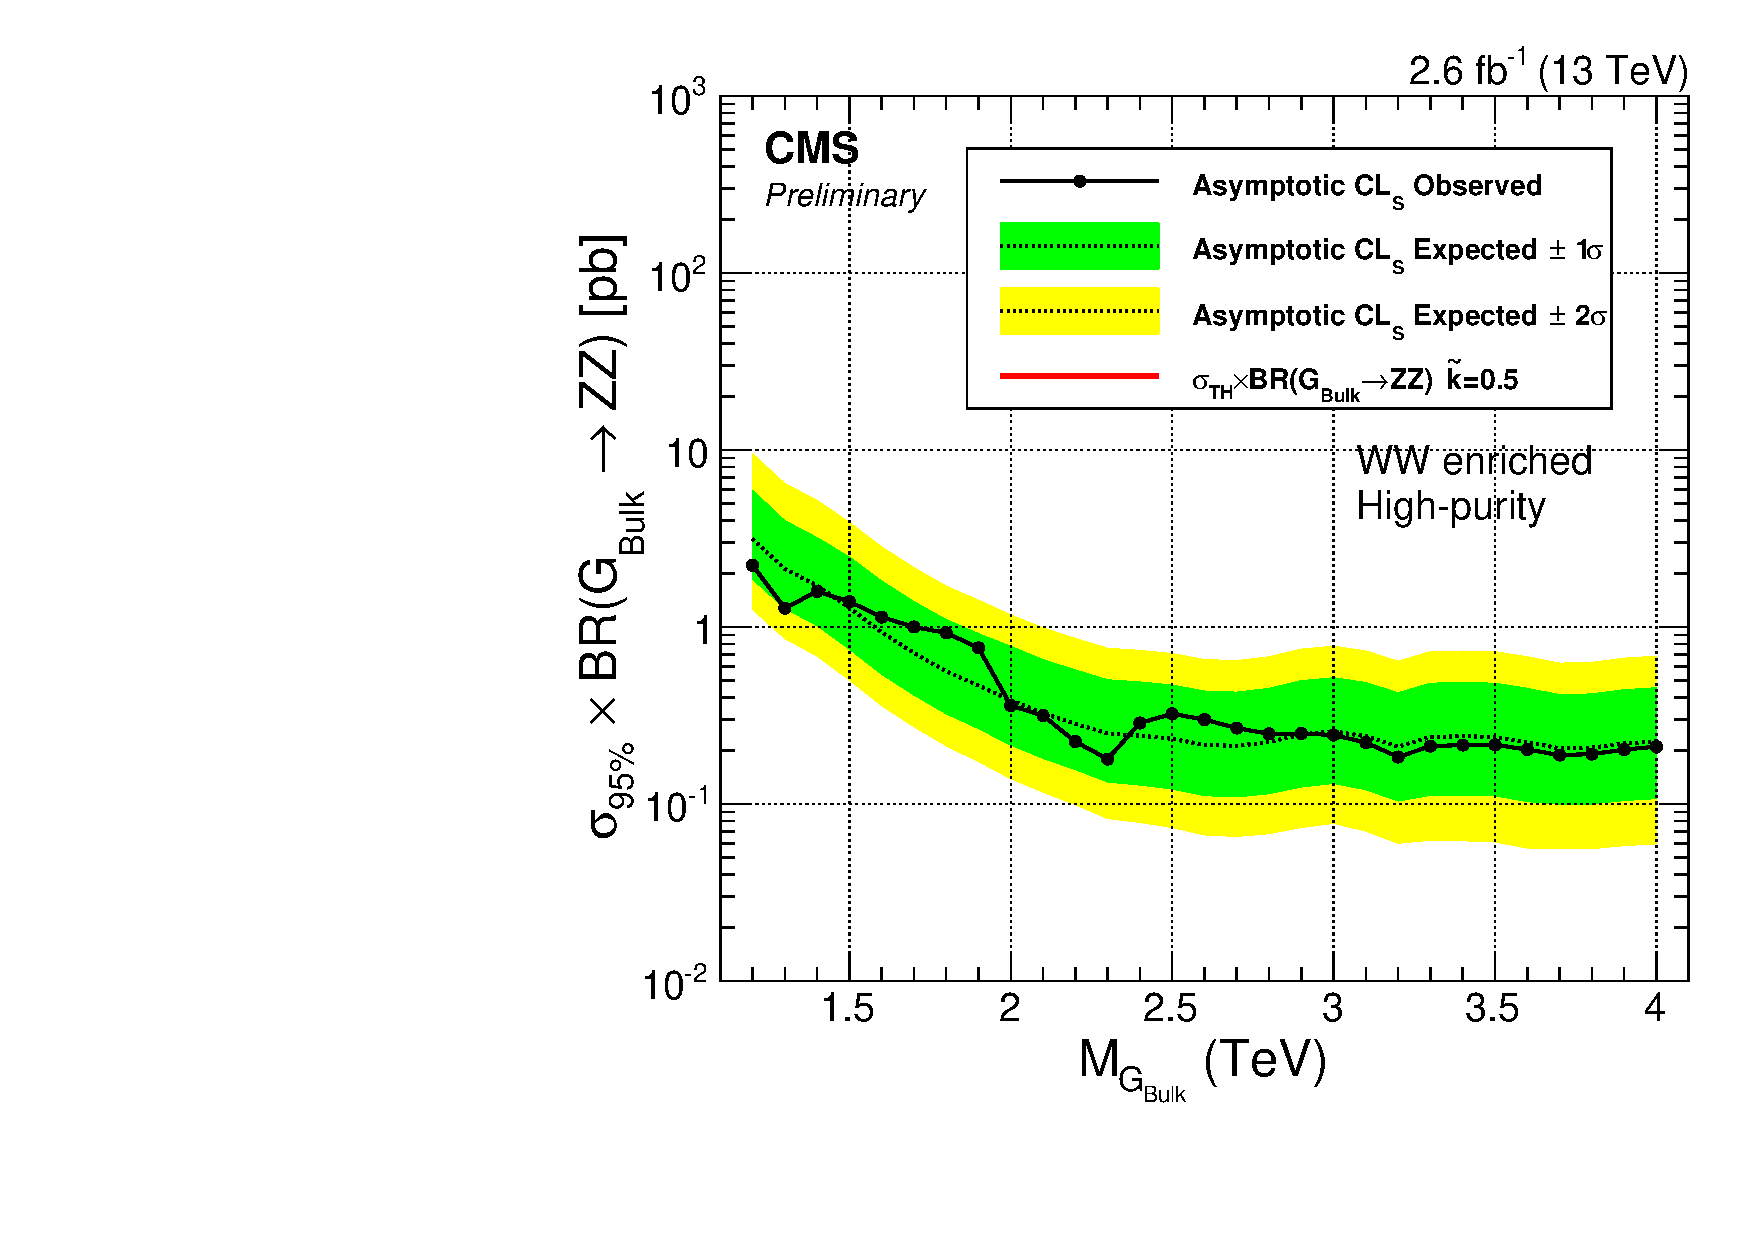
\includegraphics[width=0.32\textwidth]{figures/analysis/search1/AN-15-211/limits/brazilianFlag_BulkZZ_WWHP_13TeV_wPDF.pdf}
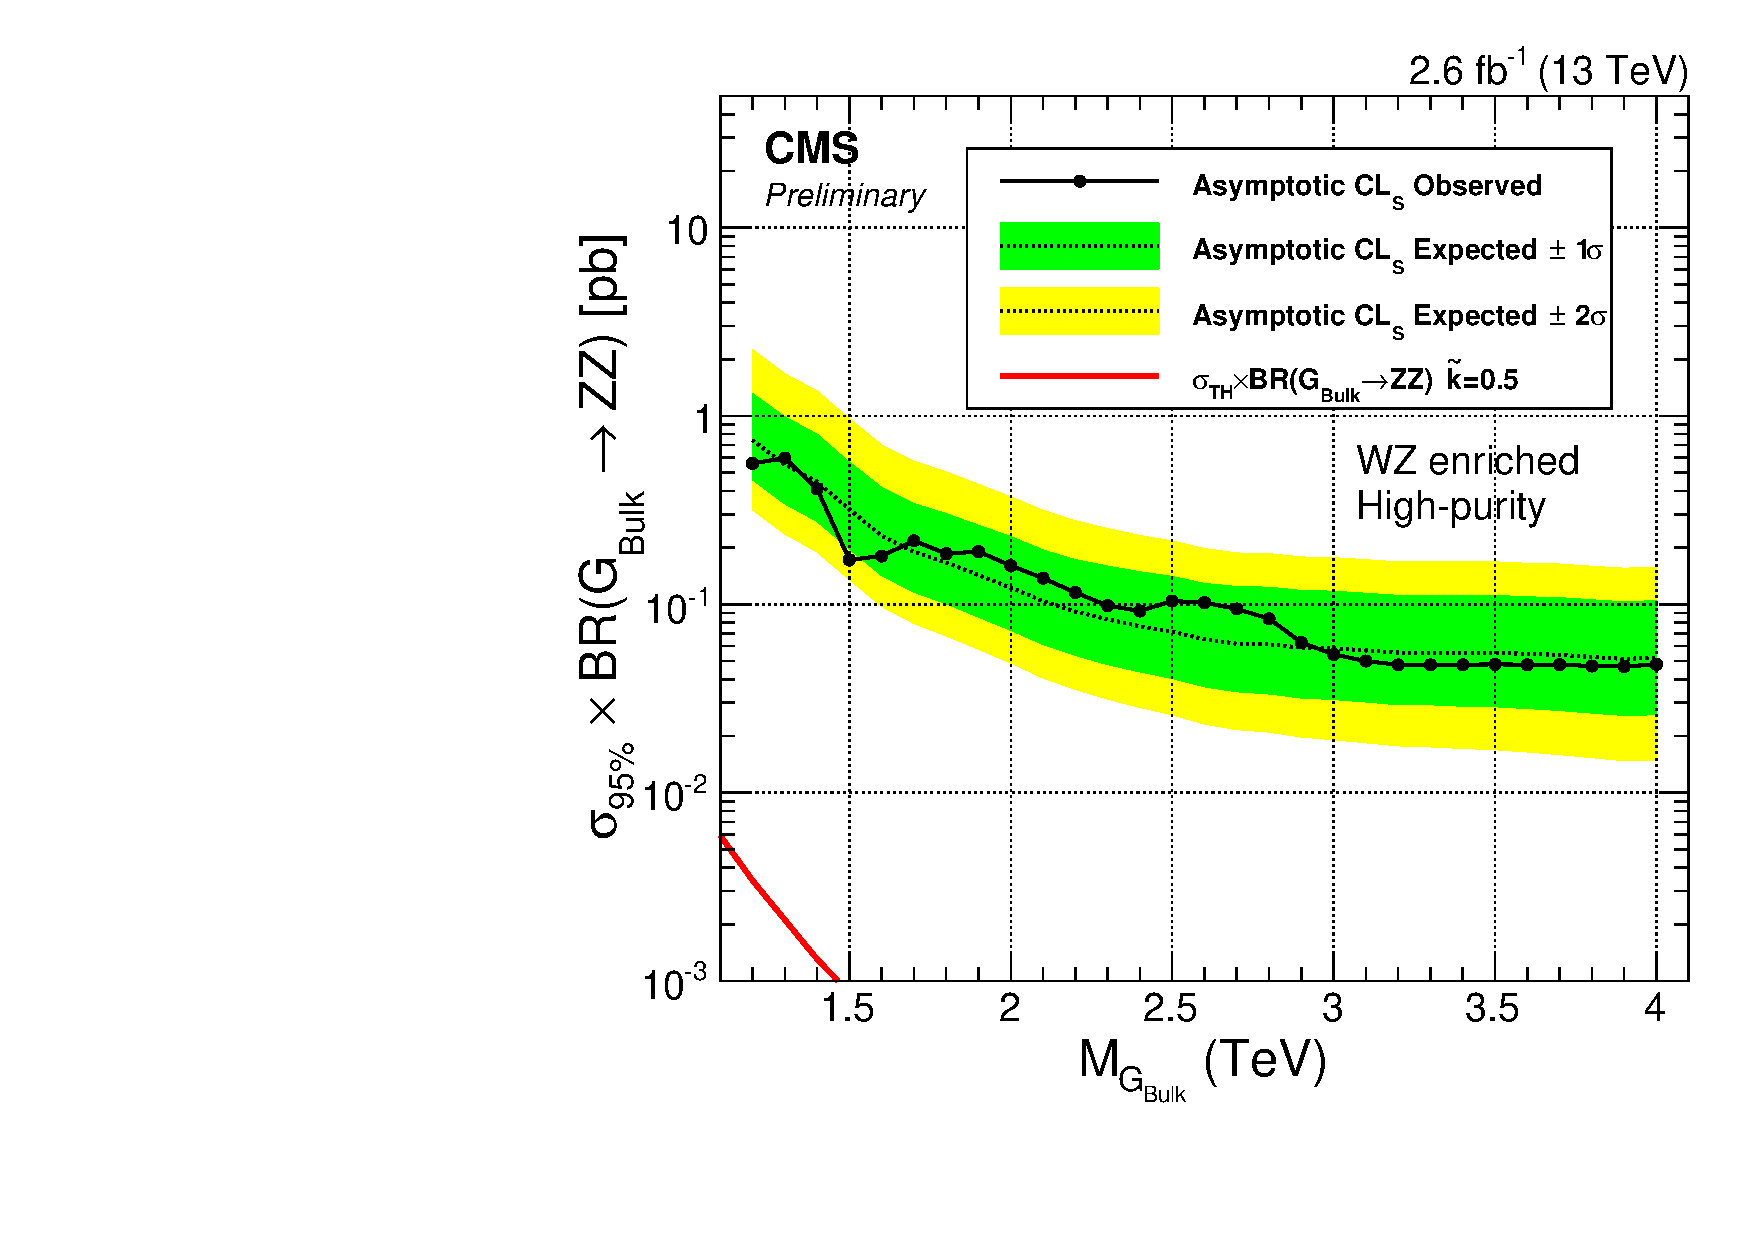
\includegraphics[width=0.32\textwidth]{figures/analysis/search1/AN-15-211/limits/brazilianFlag_BulkZZ_WZHP_13TeV_wPDF.pdf}
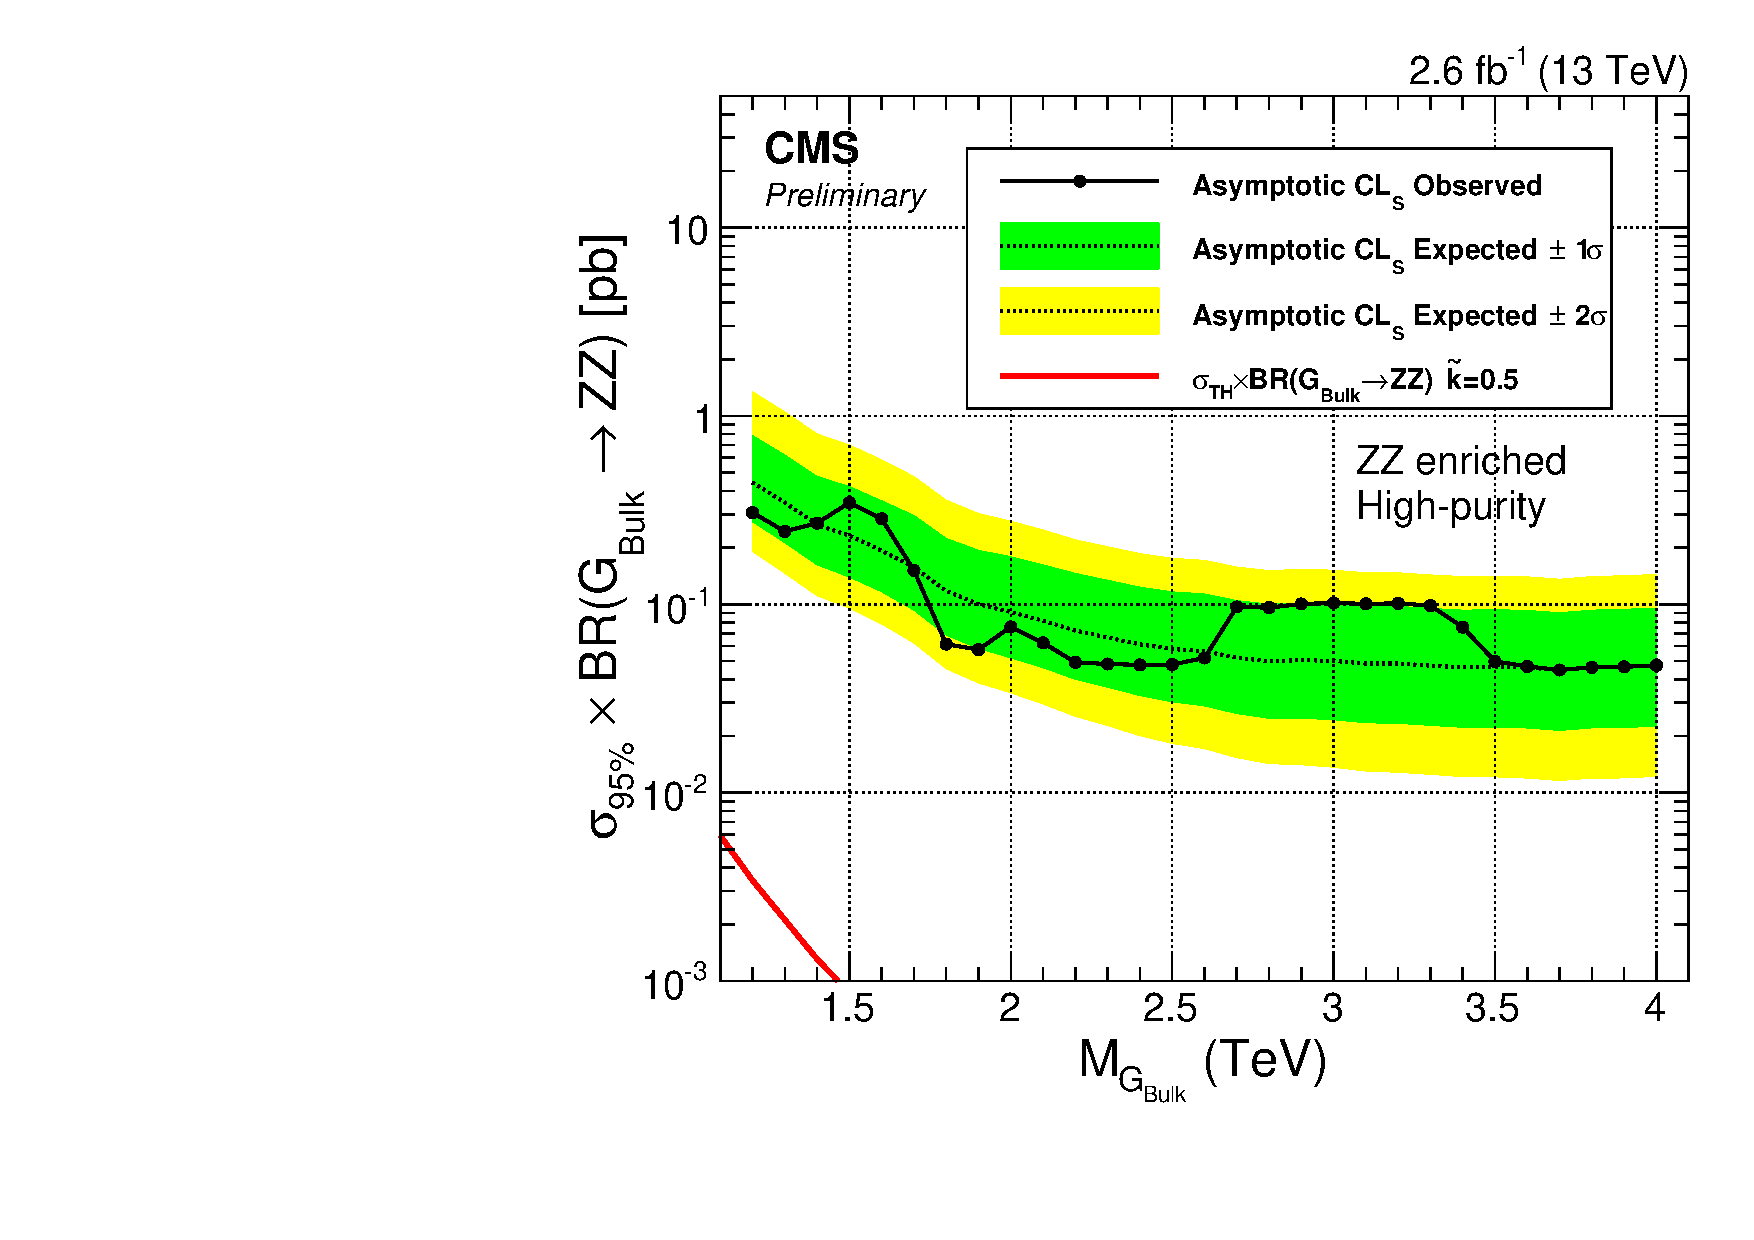
\includegraphics[width=0.32\textwidth]{figures/analysis/search1/AN-15-211/limits/brazilianFlag_BulkZZ_ZZHP_13TeV_wPDF.pdf}\\
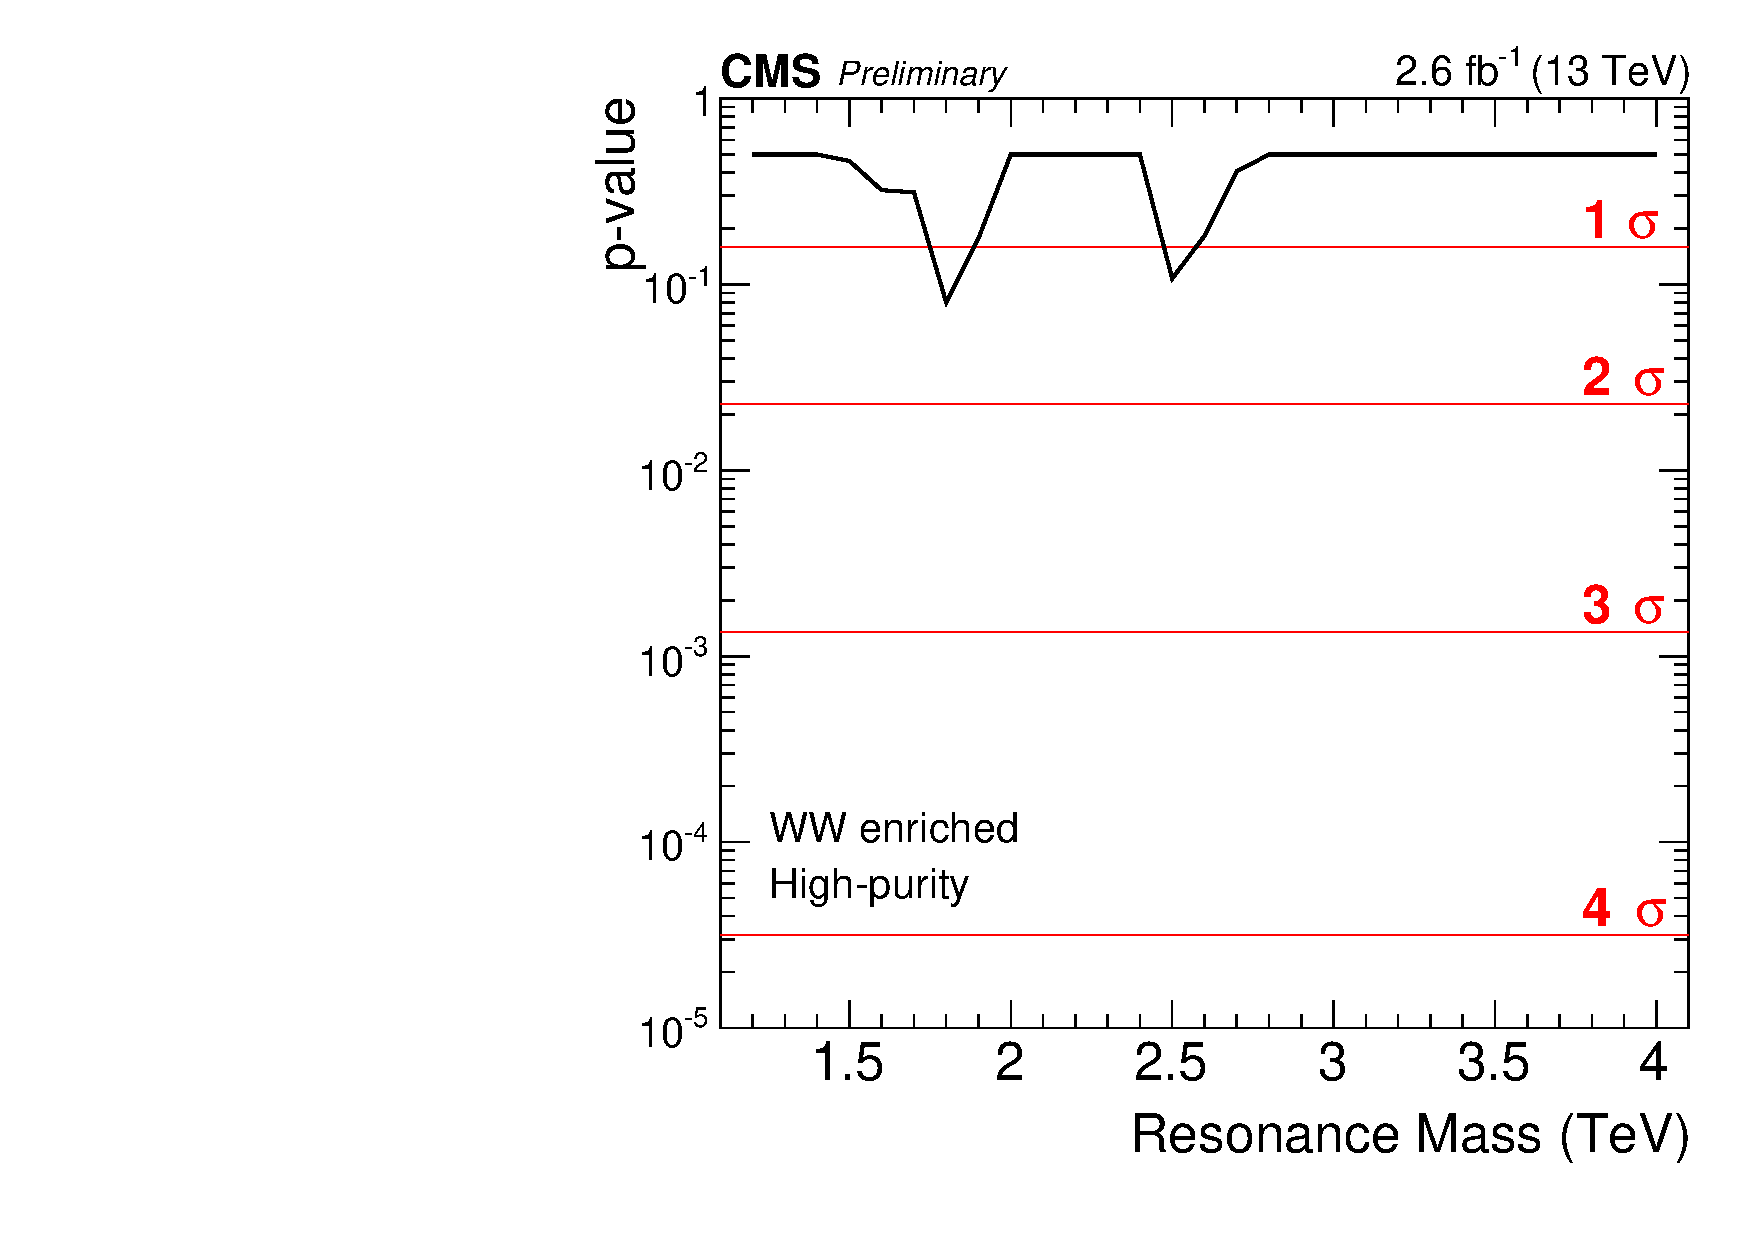
\includegraphics[width=0.32\textwidth]{figures/analysis/search1/AN-15-211/pvalues/pvalue_BulkZZinWW_high_purity.pdf}
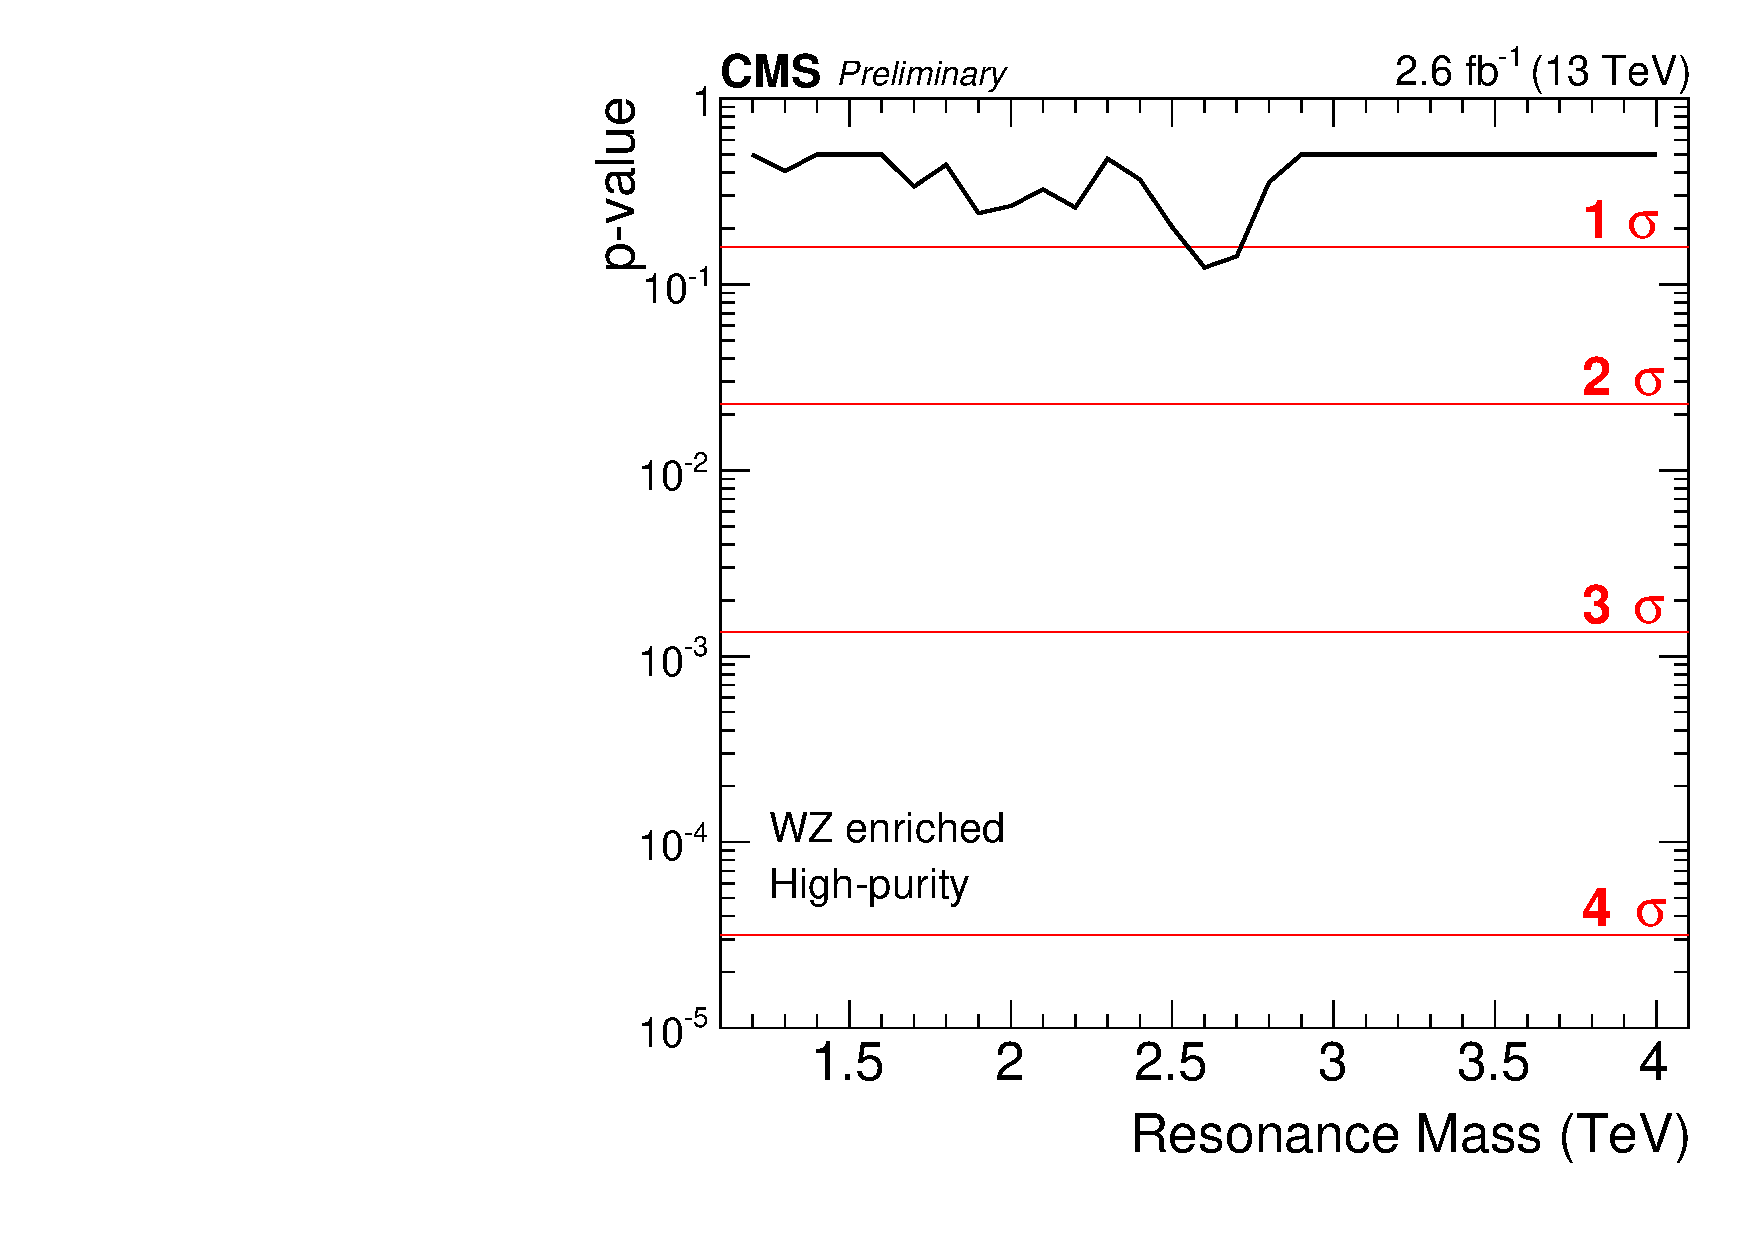
\includegraphics[width=0.32\textwidth]{figures/analysis/search1/AN-15-211/pvalues/pvalue_BulkZZinWZ_high_purity.pdf}
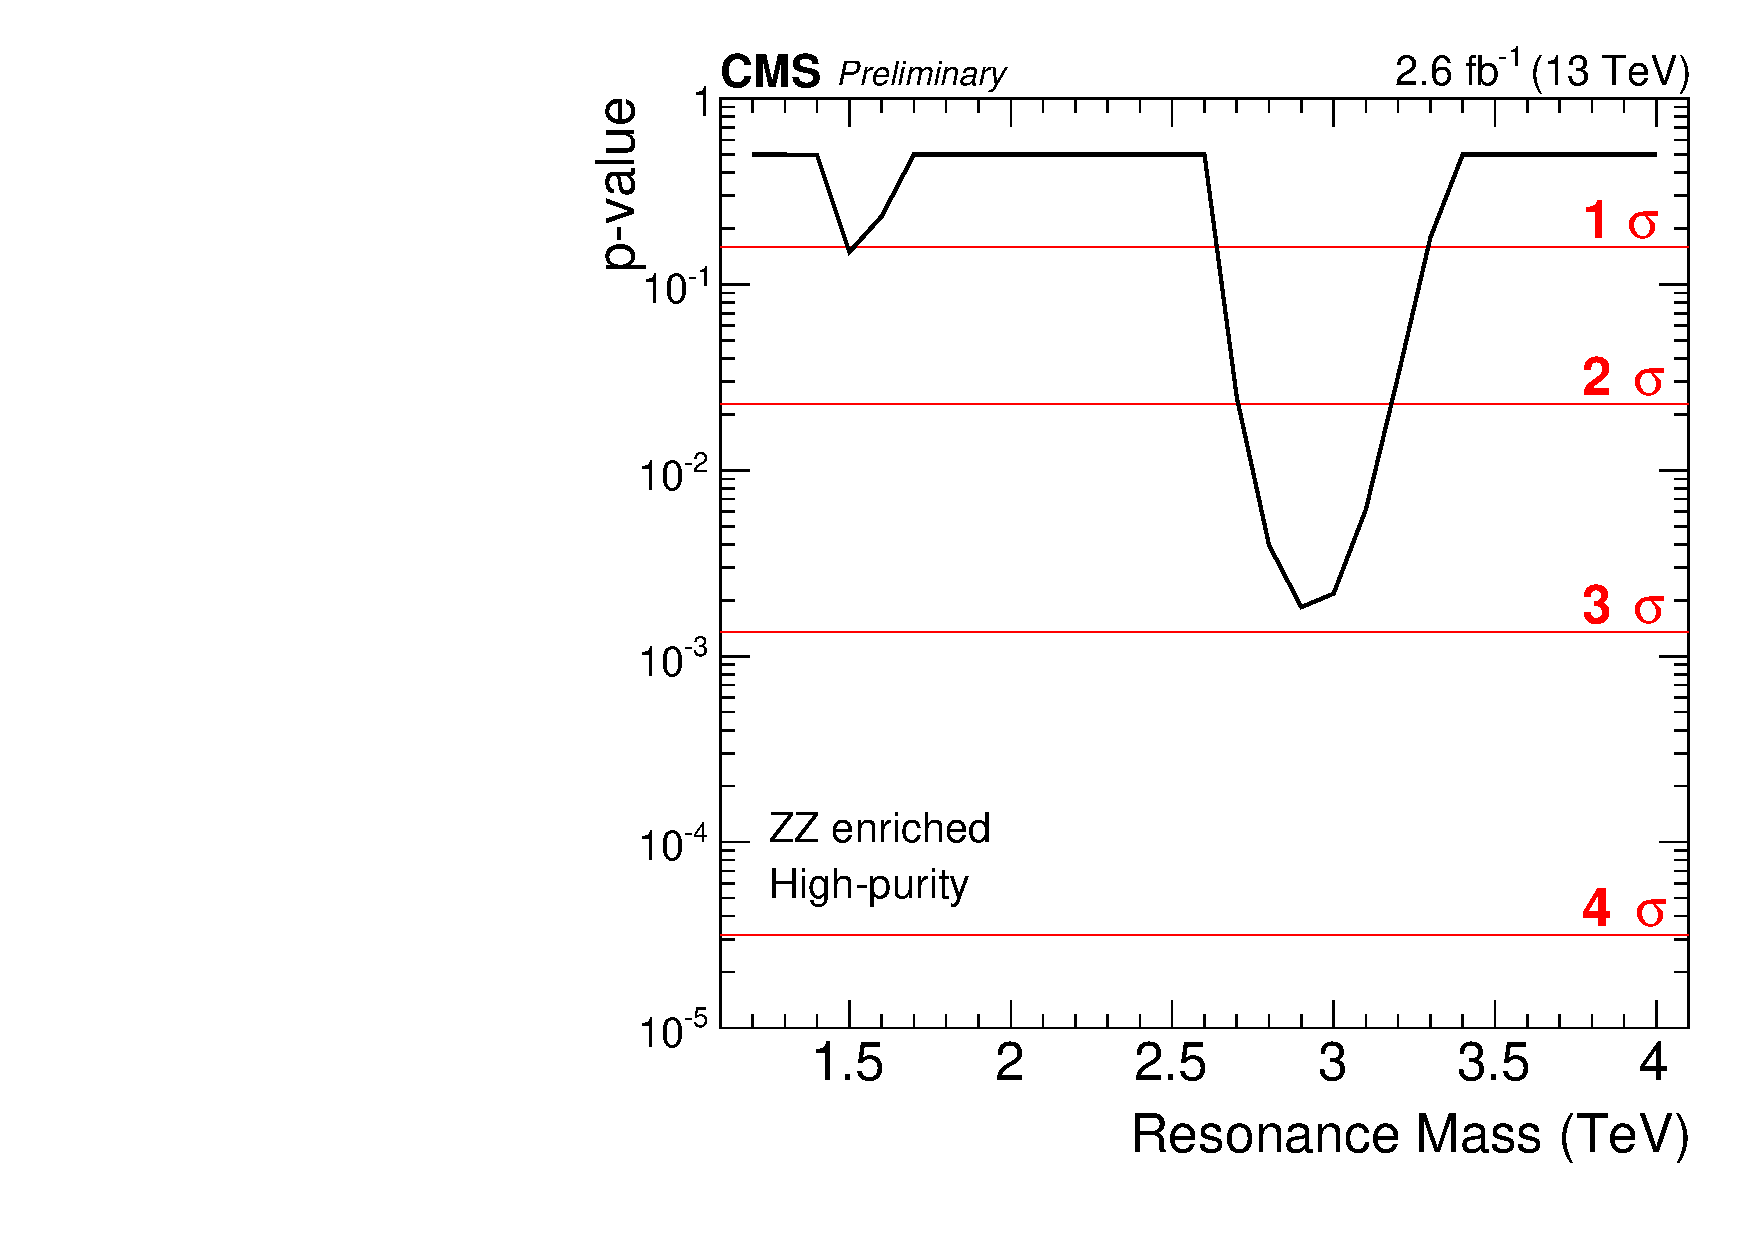
\includegraphics[width=0.32\textwidth]{figures/analysis/search1/AN-15-211/pvalues/pvalue_BulkZZinZZ_high_purity.pdf}
\caption{Expected/observed limits and corresponding p-values obtained in the different mass categories. Here for a $G\rightarrow ZZ$ signal in the HP category.}
\label{fig:searchI:Limits_HPBulkZZ}
\end{figure}



\begin{figure}[h!]
\centering
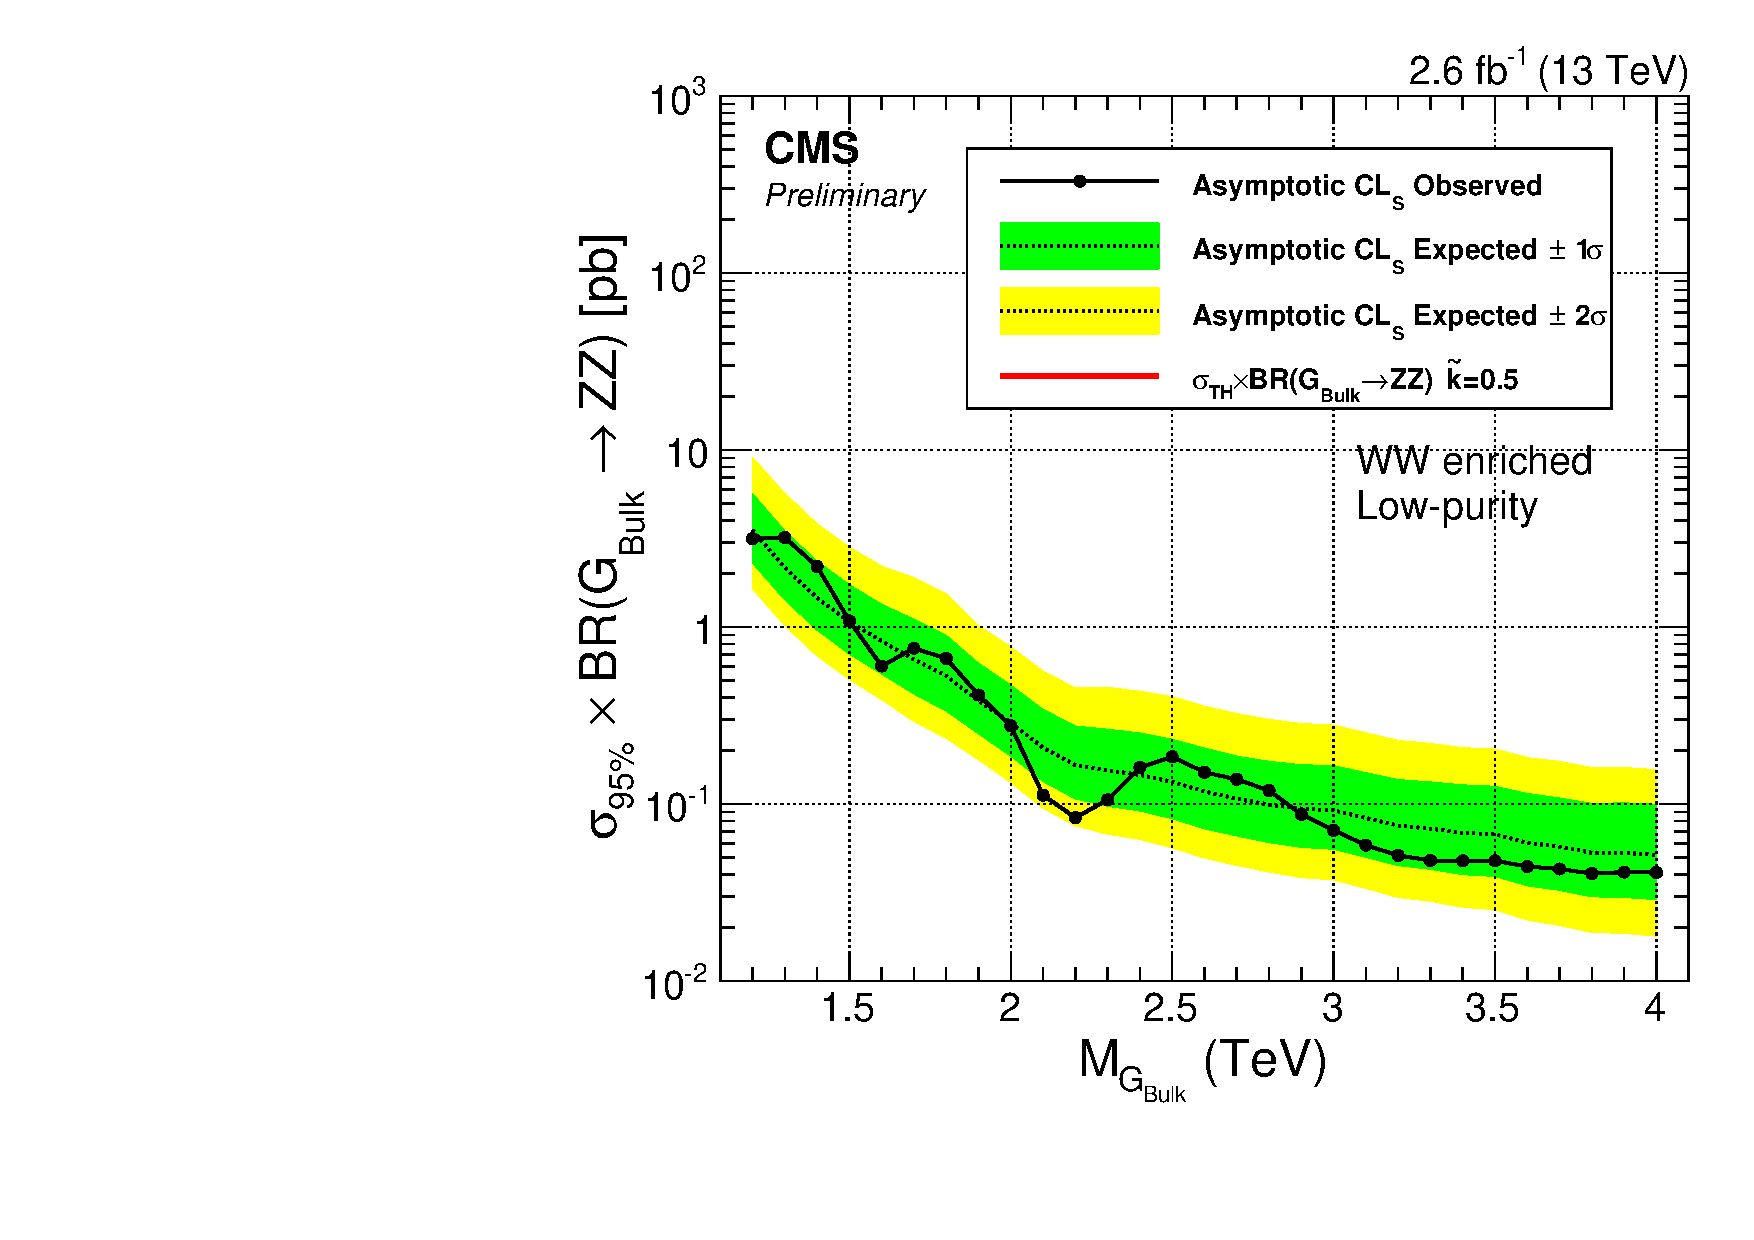
\includegraphics[width=0.32\textwidth]{figures/analysis/search1/AN-15-211/limits/brazilianFlag_BulkZZ_WWLP_13TeV_wPDF.pdf}
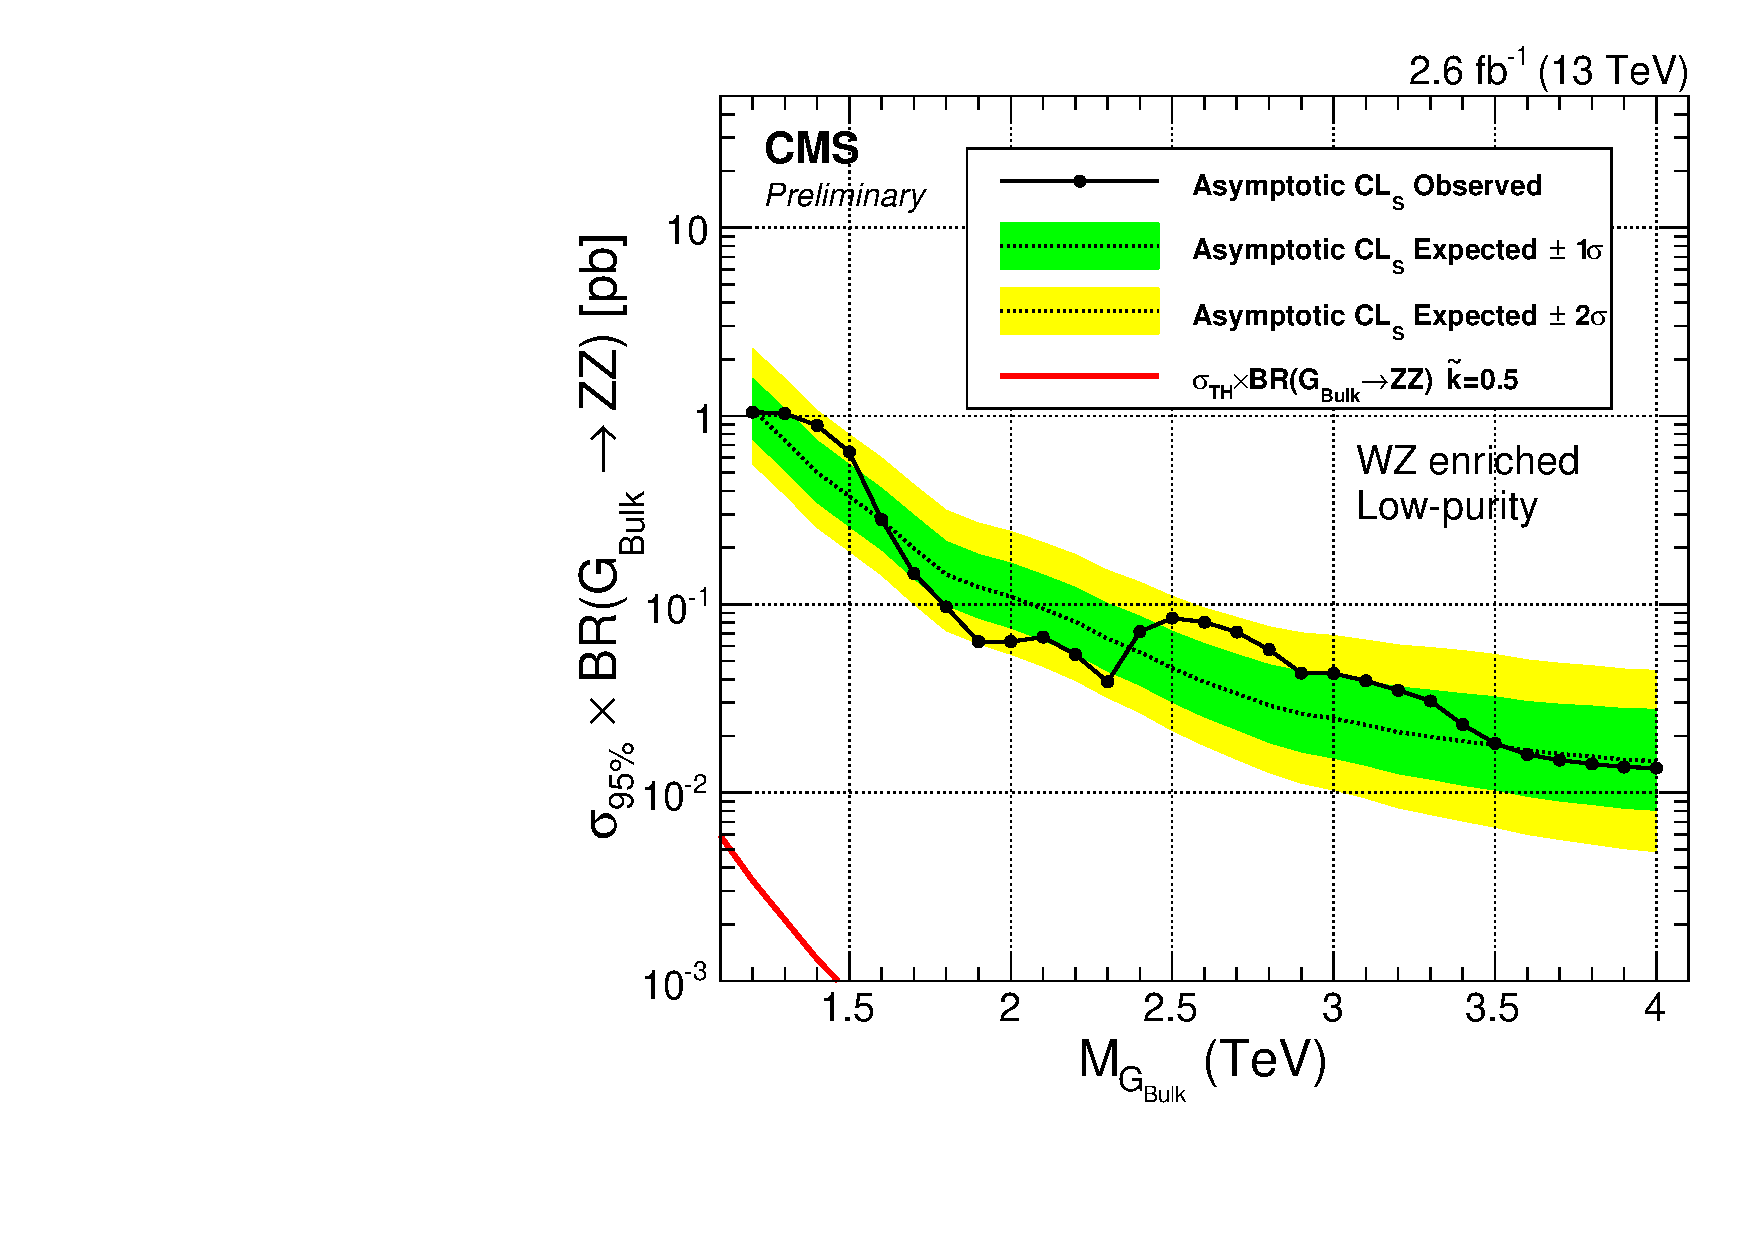
\includegraphics[width=0.32\textwidth]{figures/analysis/search1/AN-15-211/limits/brazilianFlag_BulkZZ_WZLP_13TeV_wPDF.pdf}
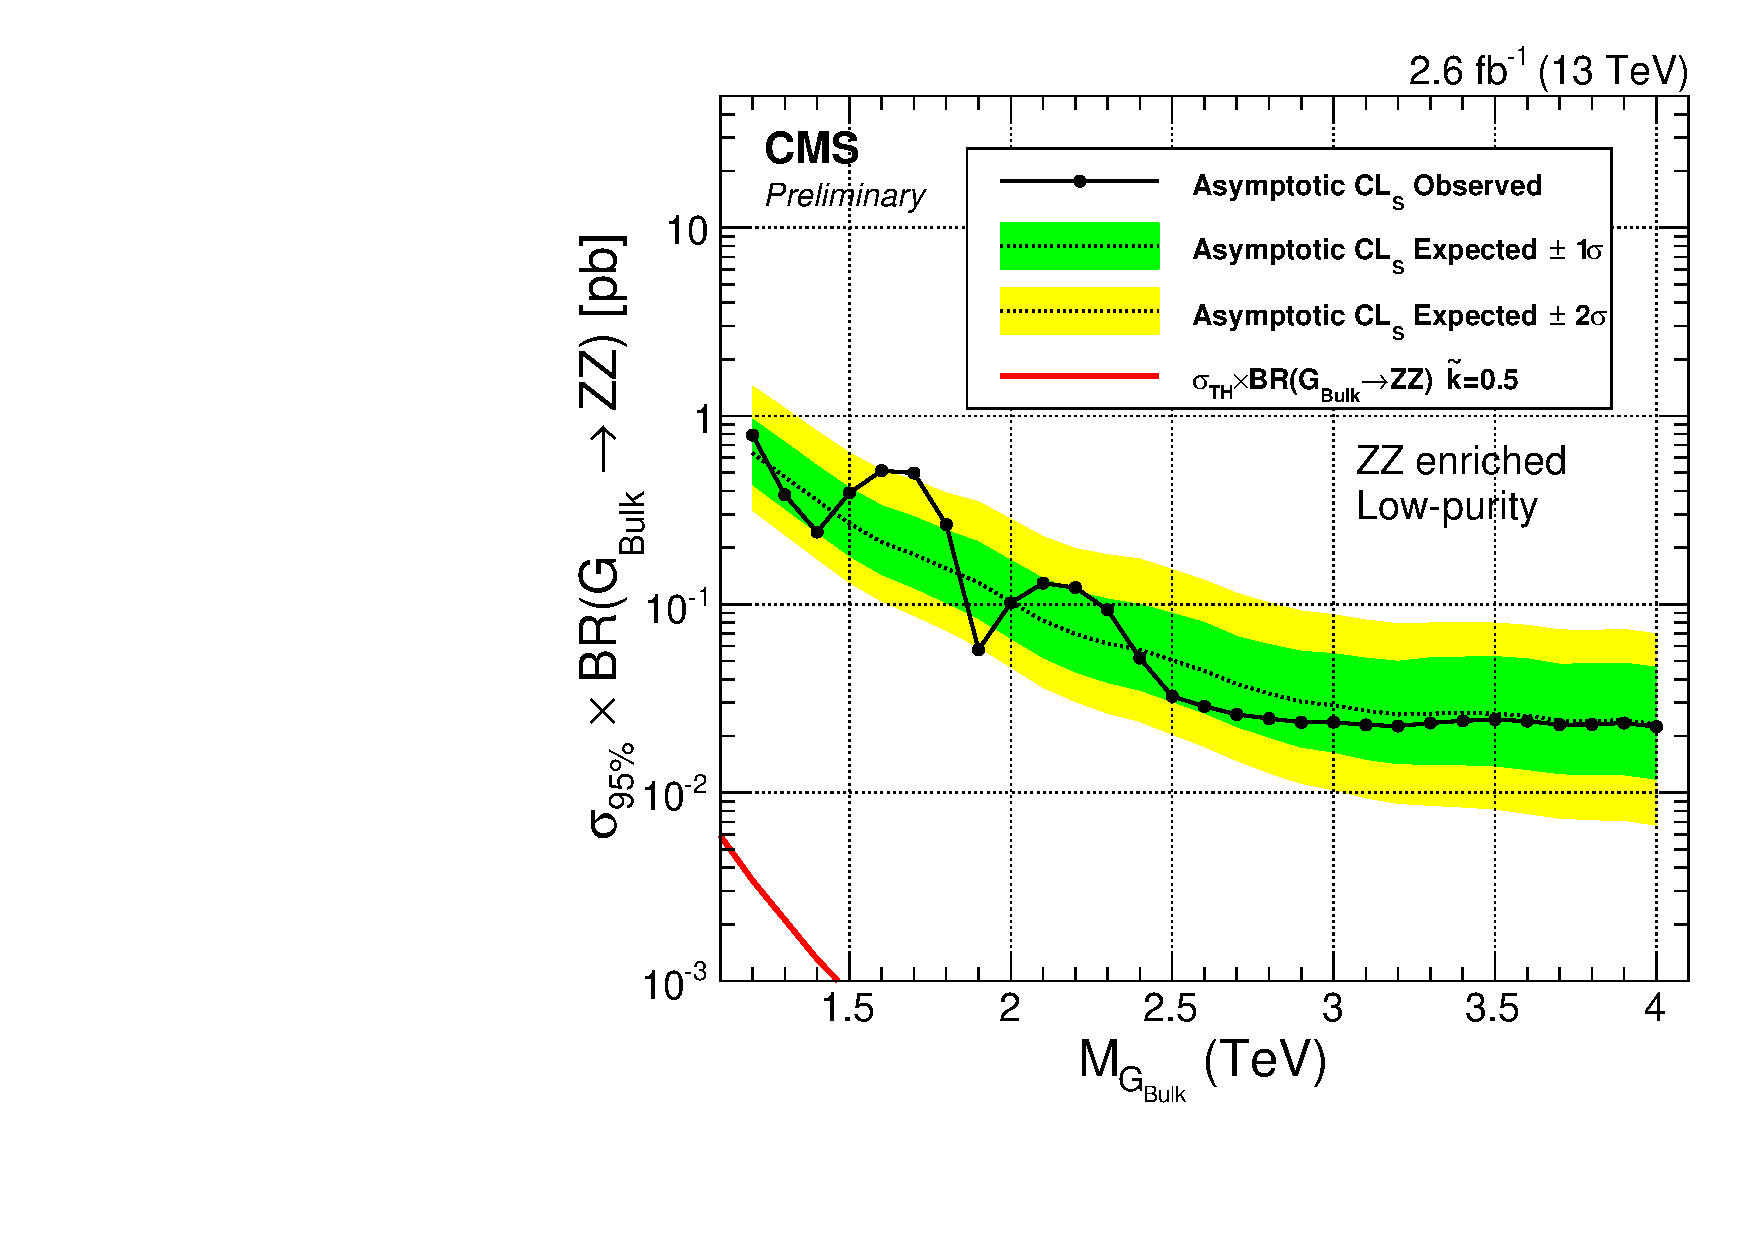
\includegraphics[width=0.32\textwidth]{figures/analysis/search1/AN-15-211/limits/brazilianFlag_BulkZZ_ZZLP_13TeV_wPDF.pdf}\\
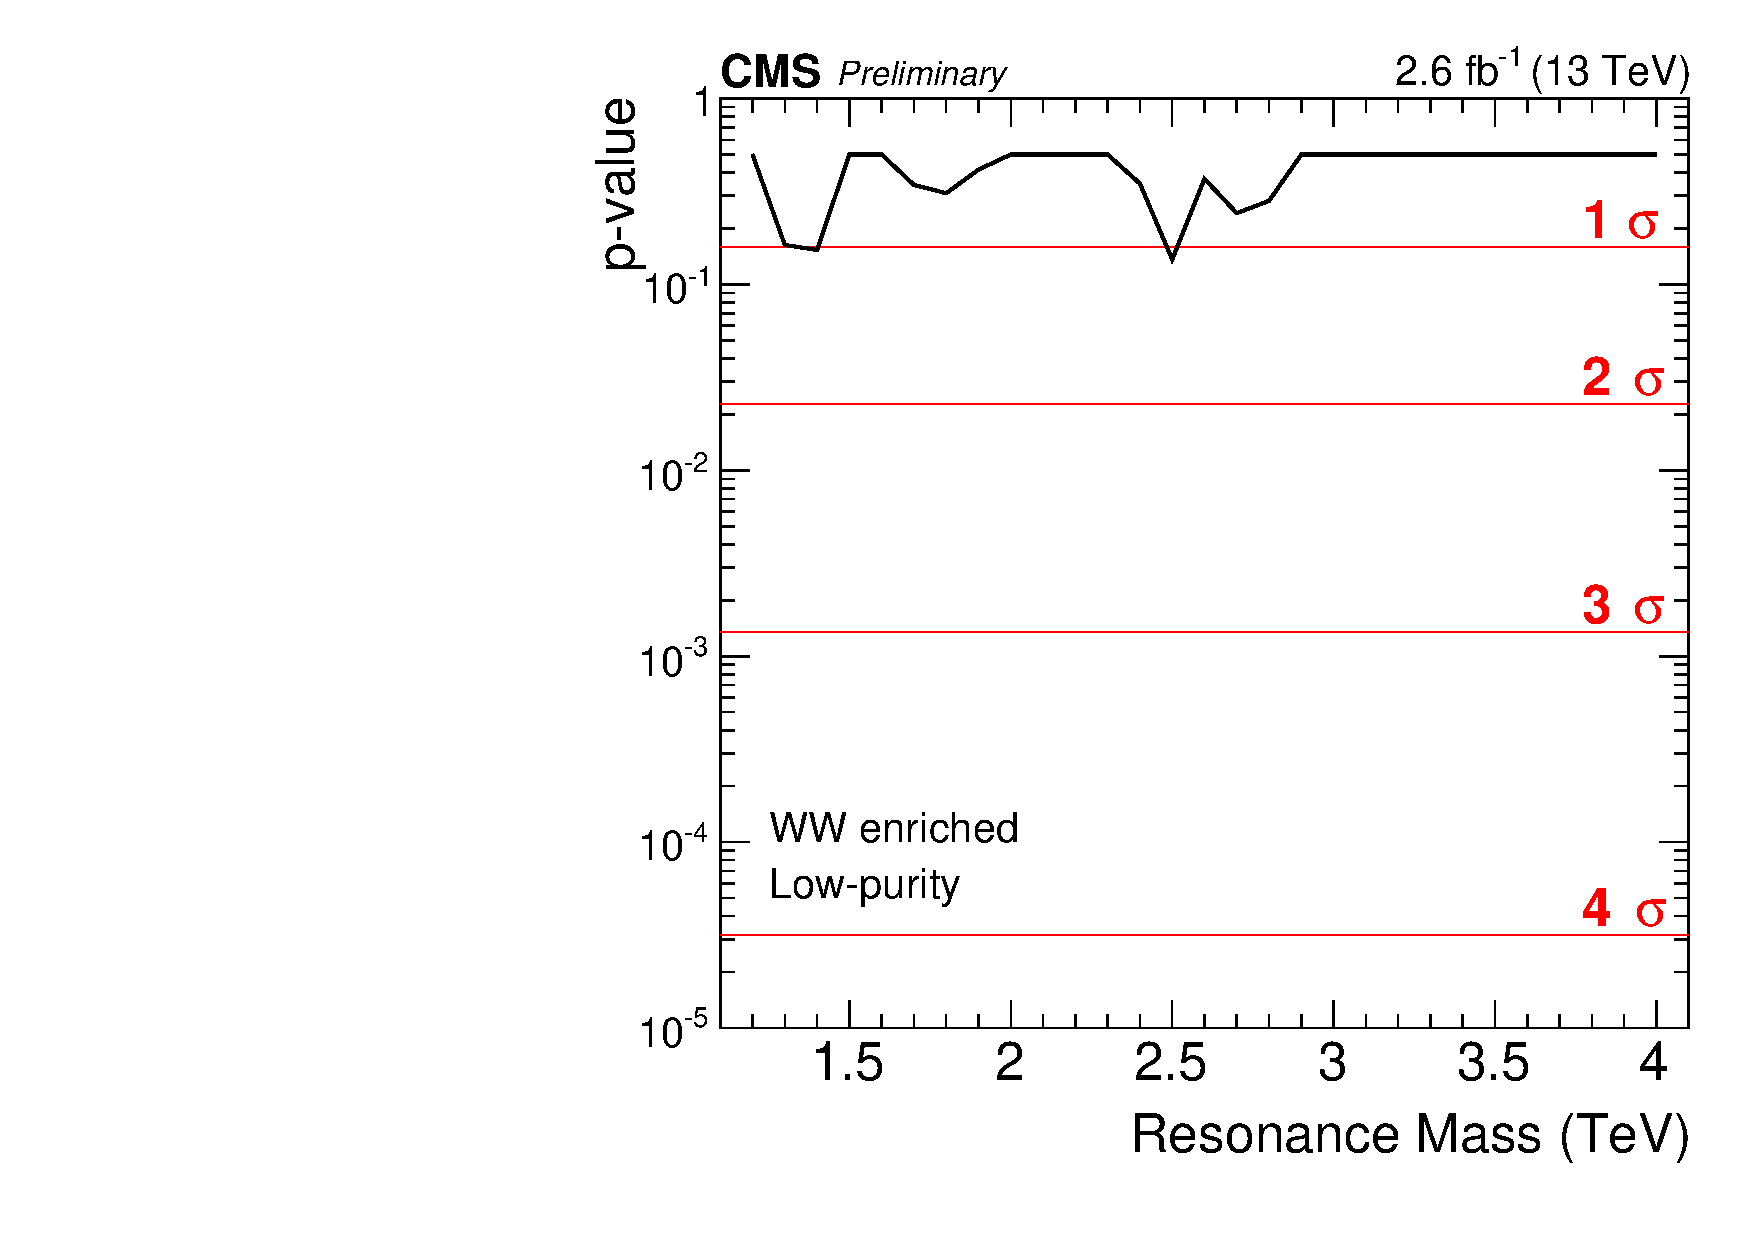
\includegraphics[width=0.32\textwidth]{figures/analysis/search1/AN-15-211/pvalues/pvalue_BulkZZinWW_low_purity.pdf}
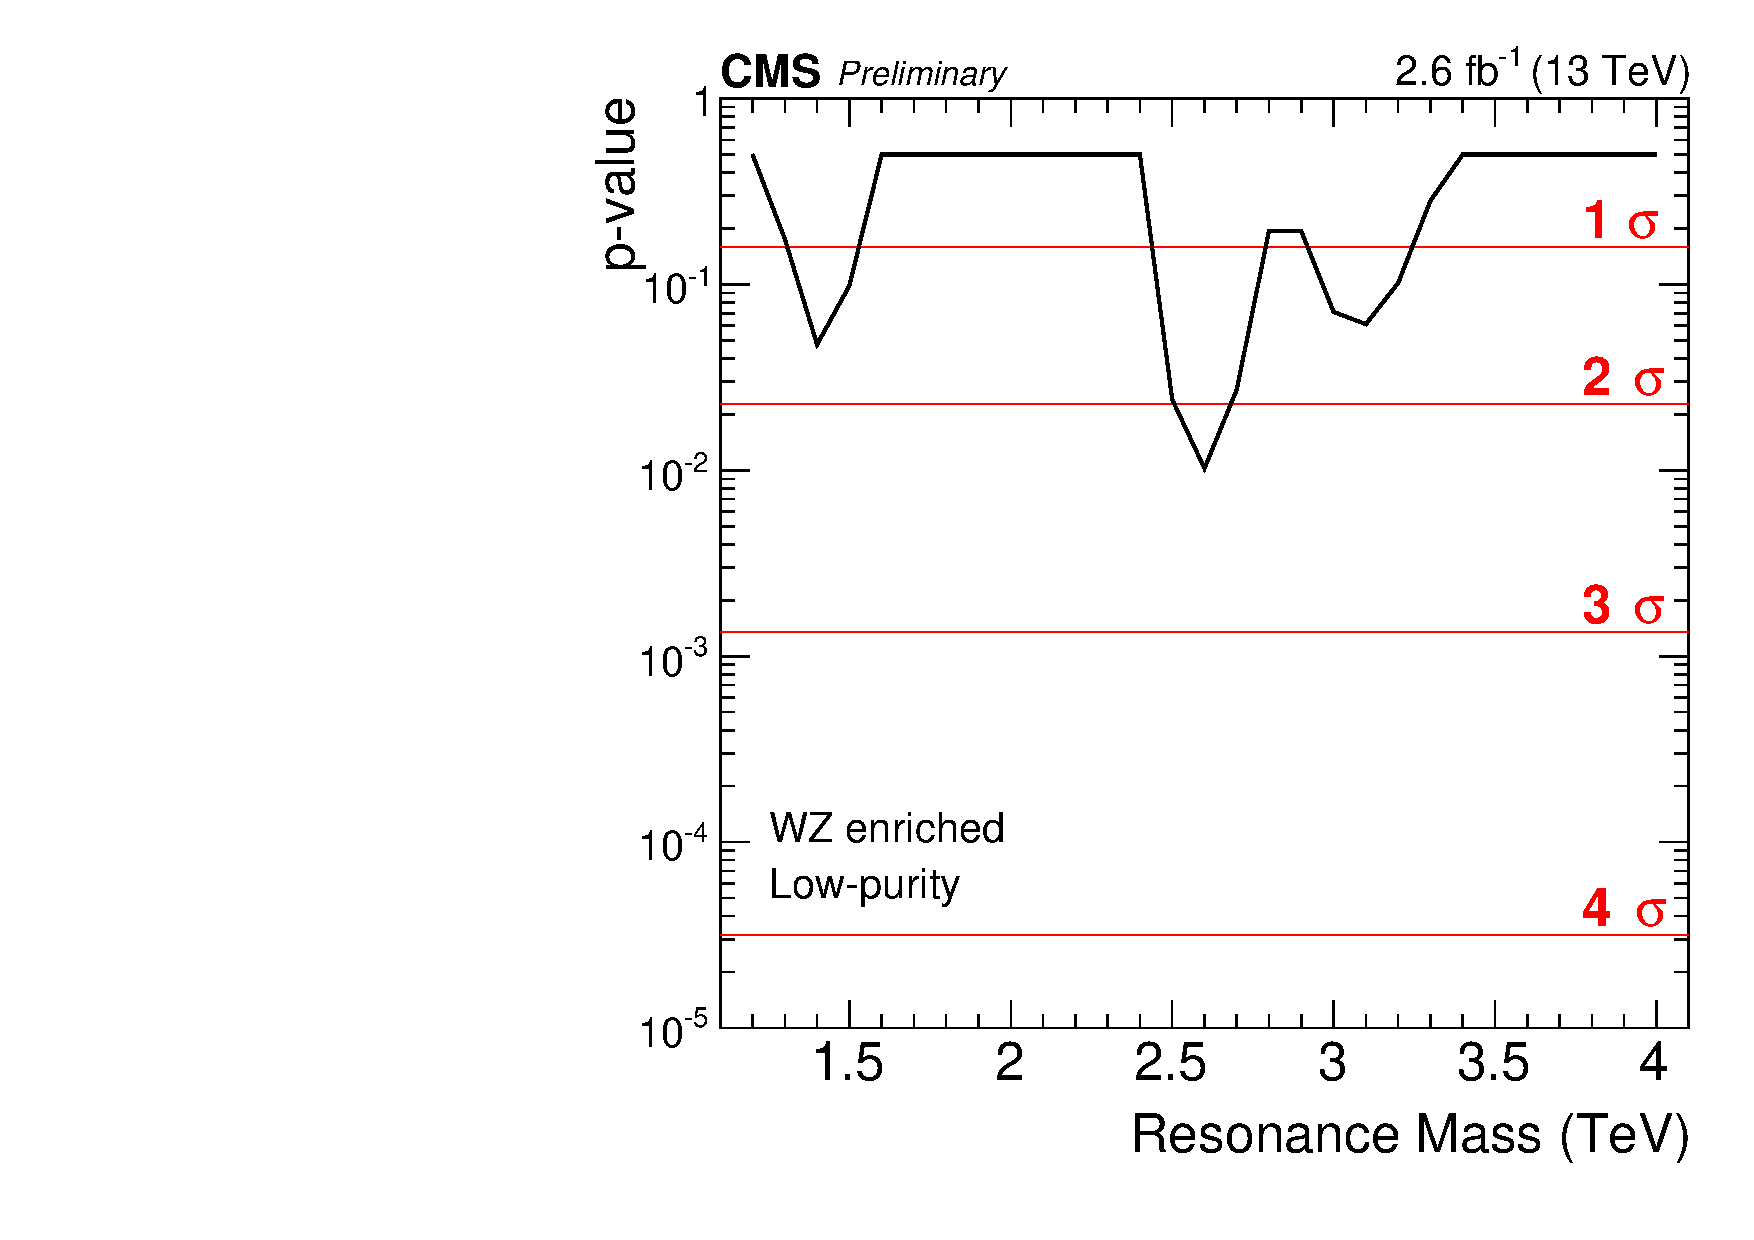
\includegraphics[width=0.32\textwidth]{figures/analysis/search1/AN-15-211/pvalues/pvalue_BulkZZinWZ_low_purity.pdf}
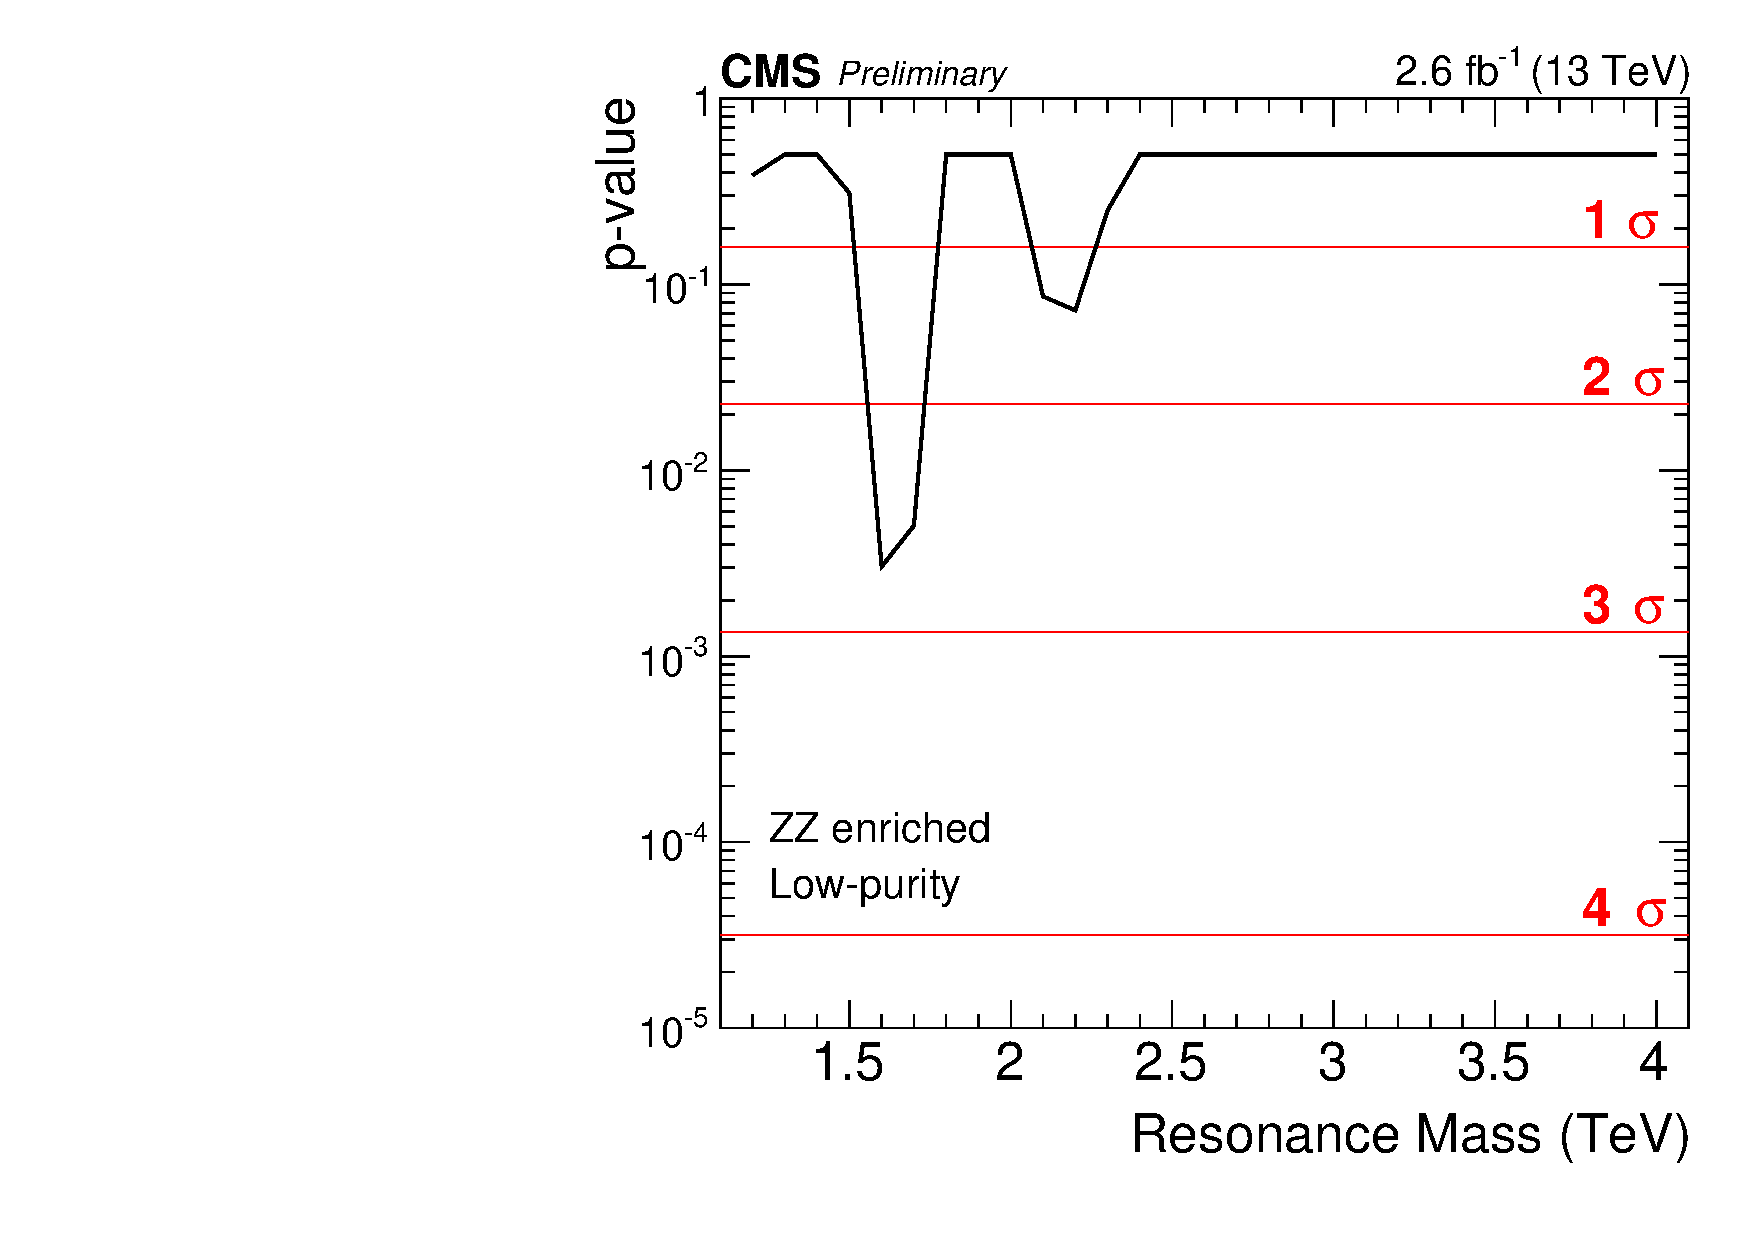
\includegraphics[width=0.32\textwidth]{figures/analysis/search1/AN-15-211/pvalues/pvalue_BulkZZinZZ_low_purity.pdf}
\caption{Expected/observed limits and corresponding p-values obtained in the different mass categories. Here for a $G\rightarrow ZZ$ signal in the LP category.}
\label{fig:searchI:Limits_LPBulkZZ}
\end{figure}





\begin{figure}[h!]
\centering
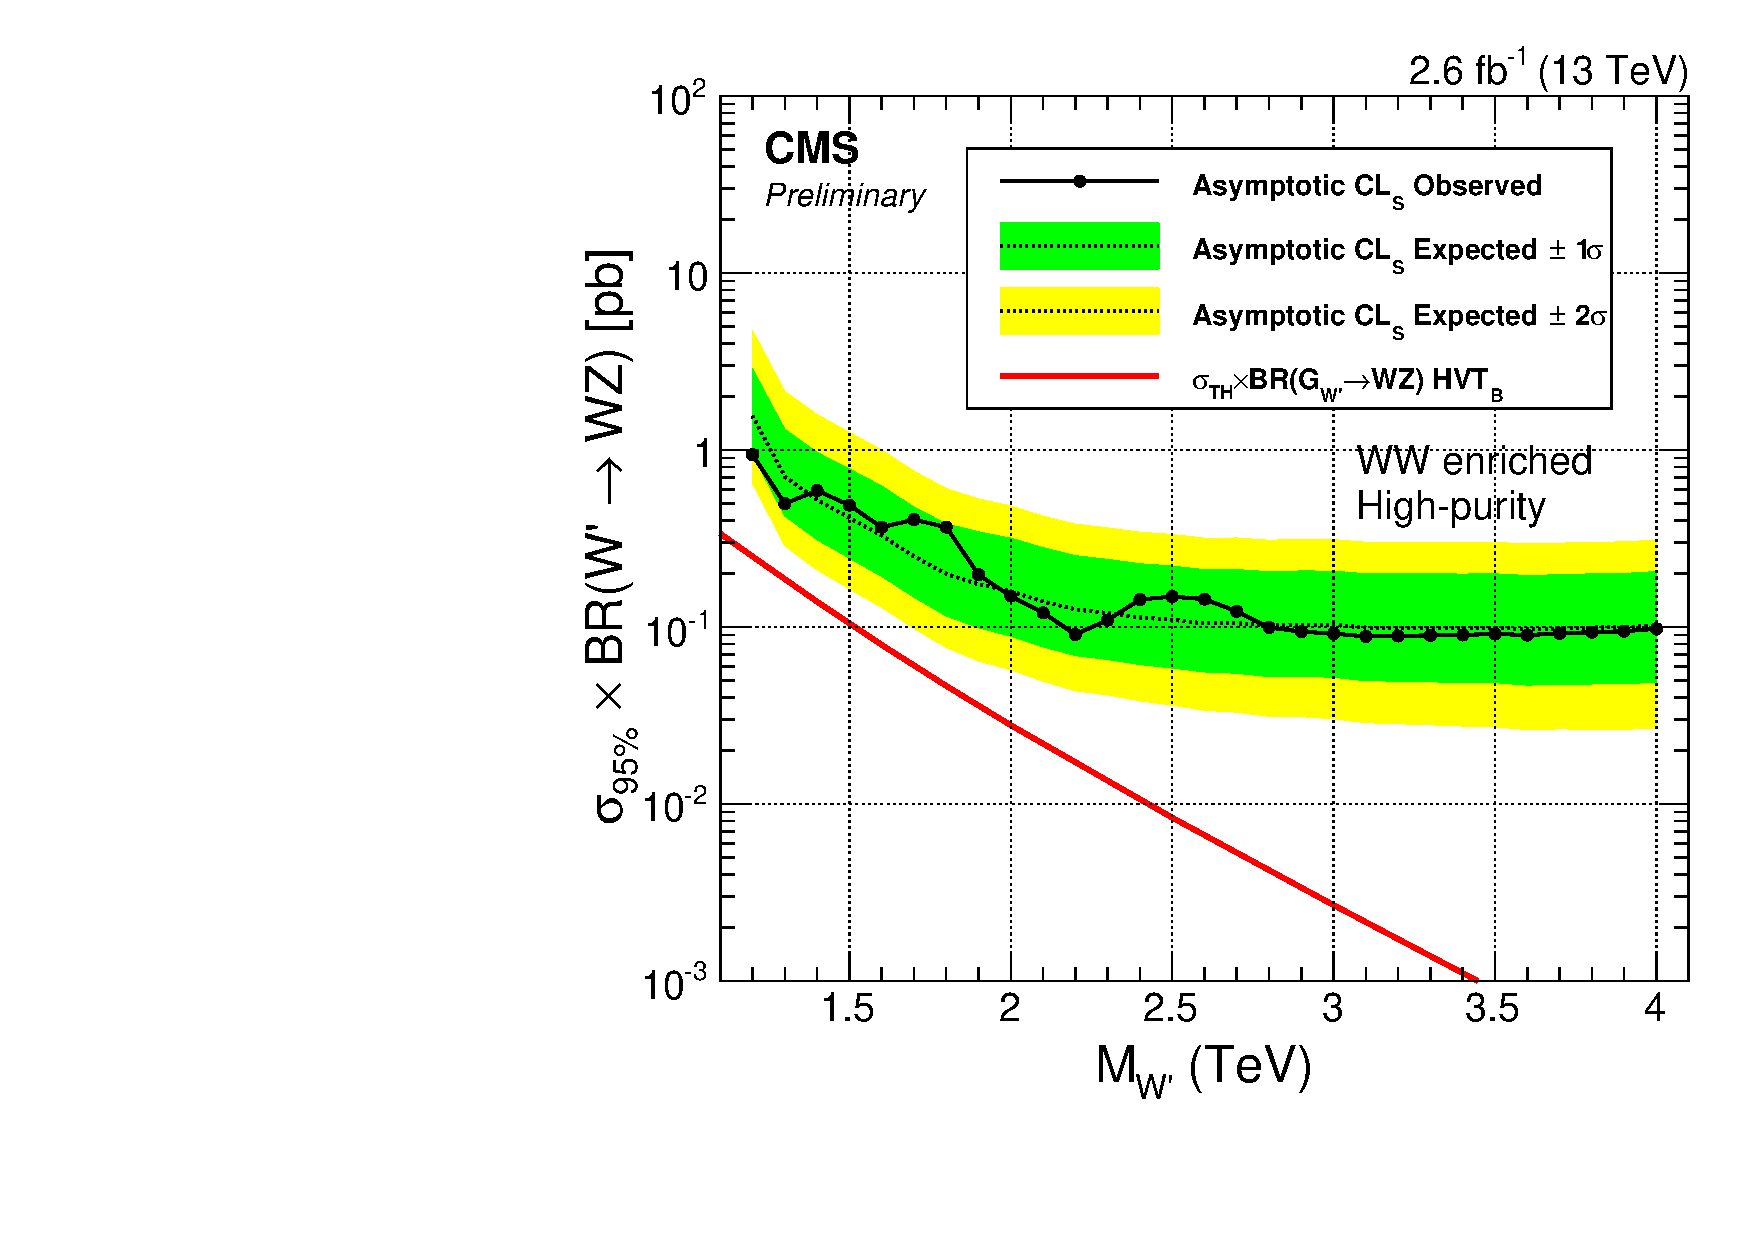
\includegraphics[width=0.32\textwidth]{figures/analysis/search1/AN-15-211/limits/brazilianFlag_WZ_WWHP_13TeV_wPDF.pdf}
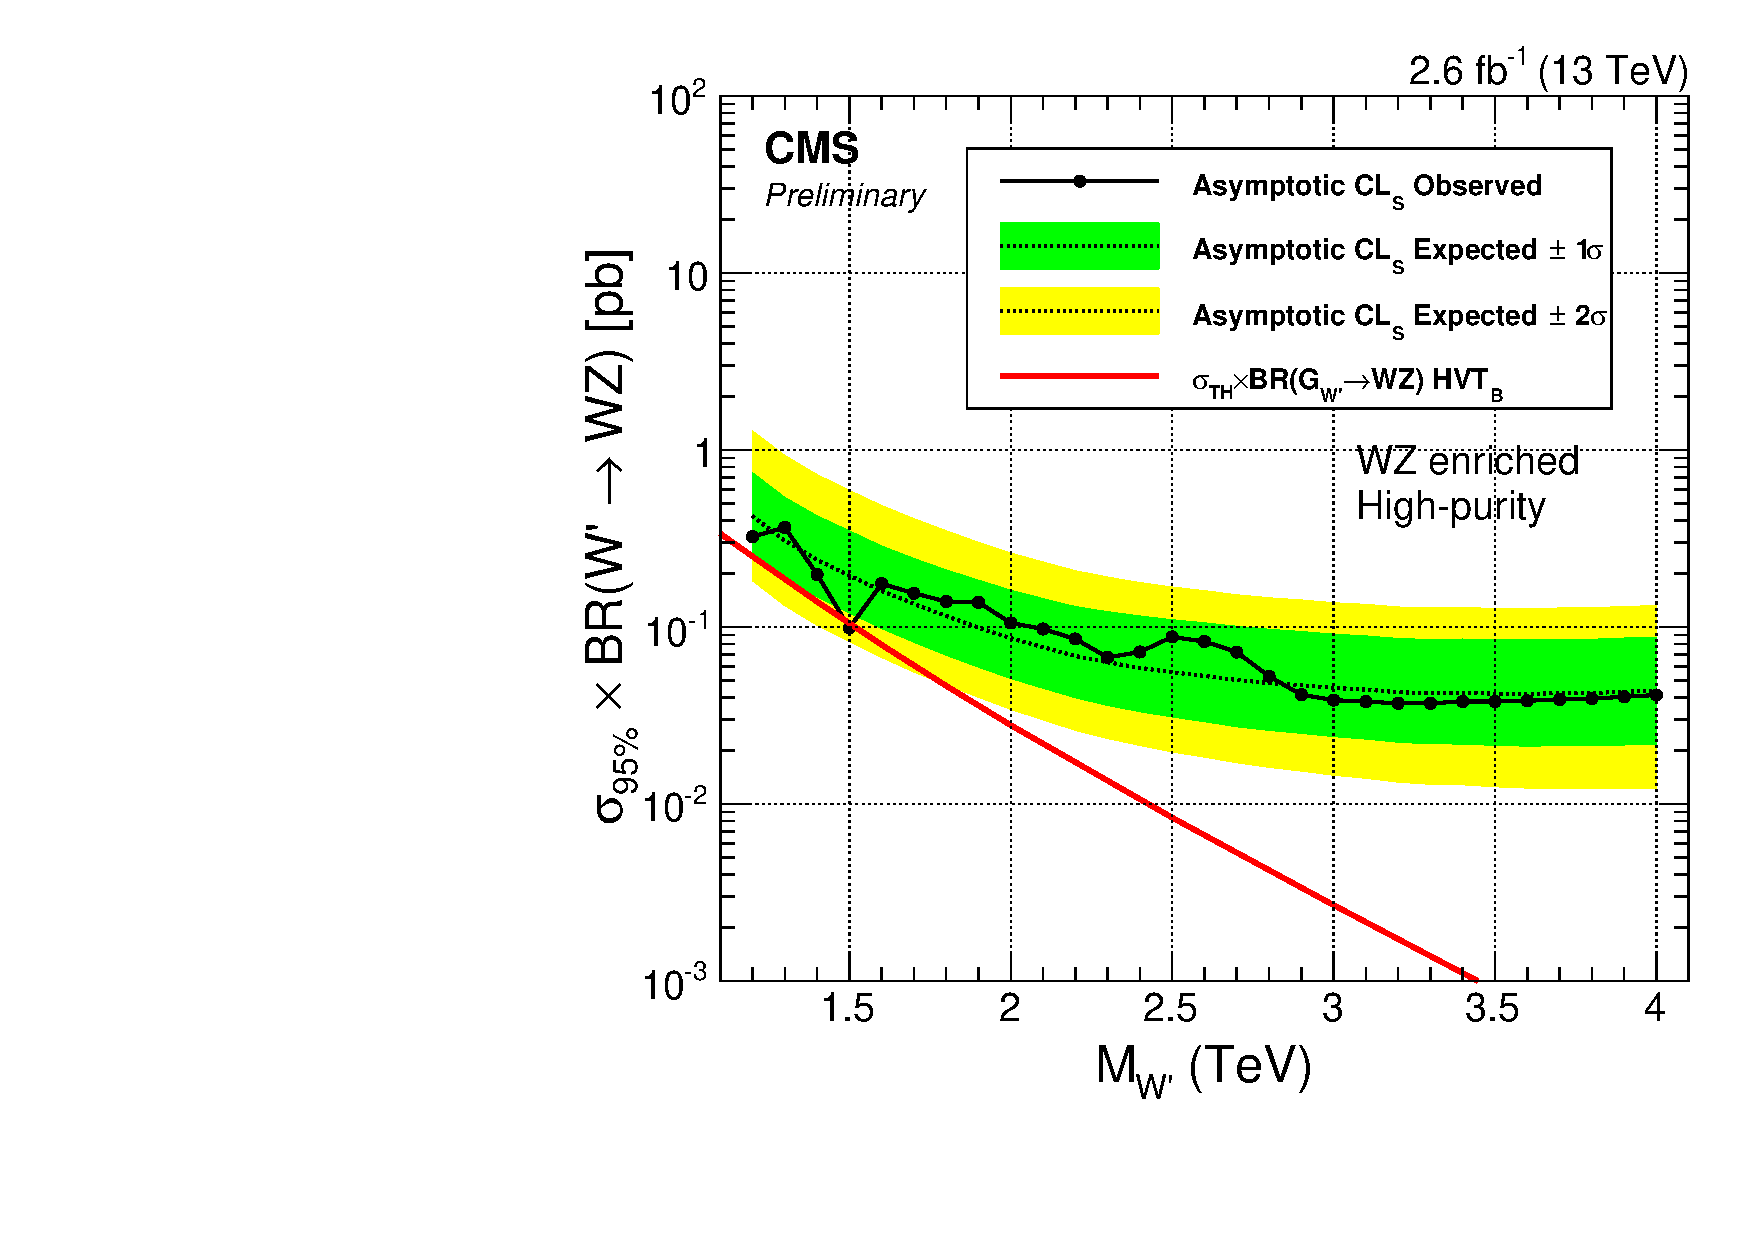
\includegraphics[width=0.32\textwidth]{figures/analysis/search1/AN-15-211/limits/brazilianFlag_WZ_WZHP_13TeV_wPDF.pdf}
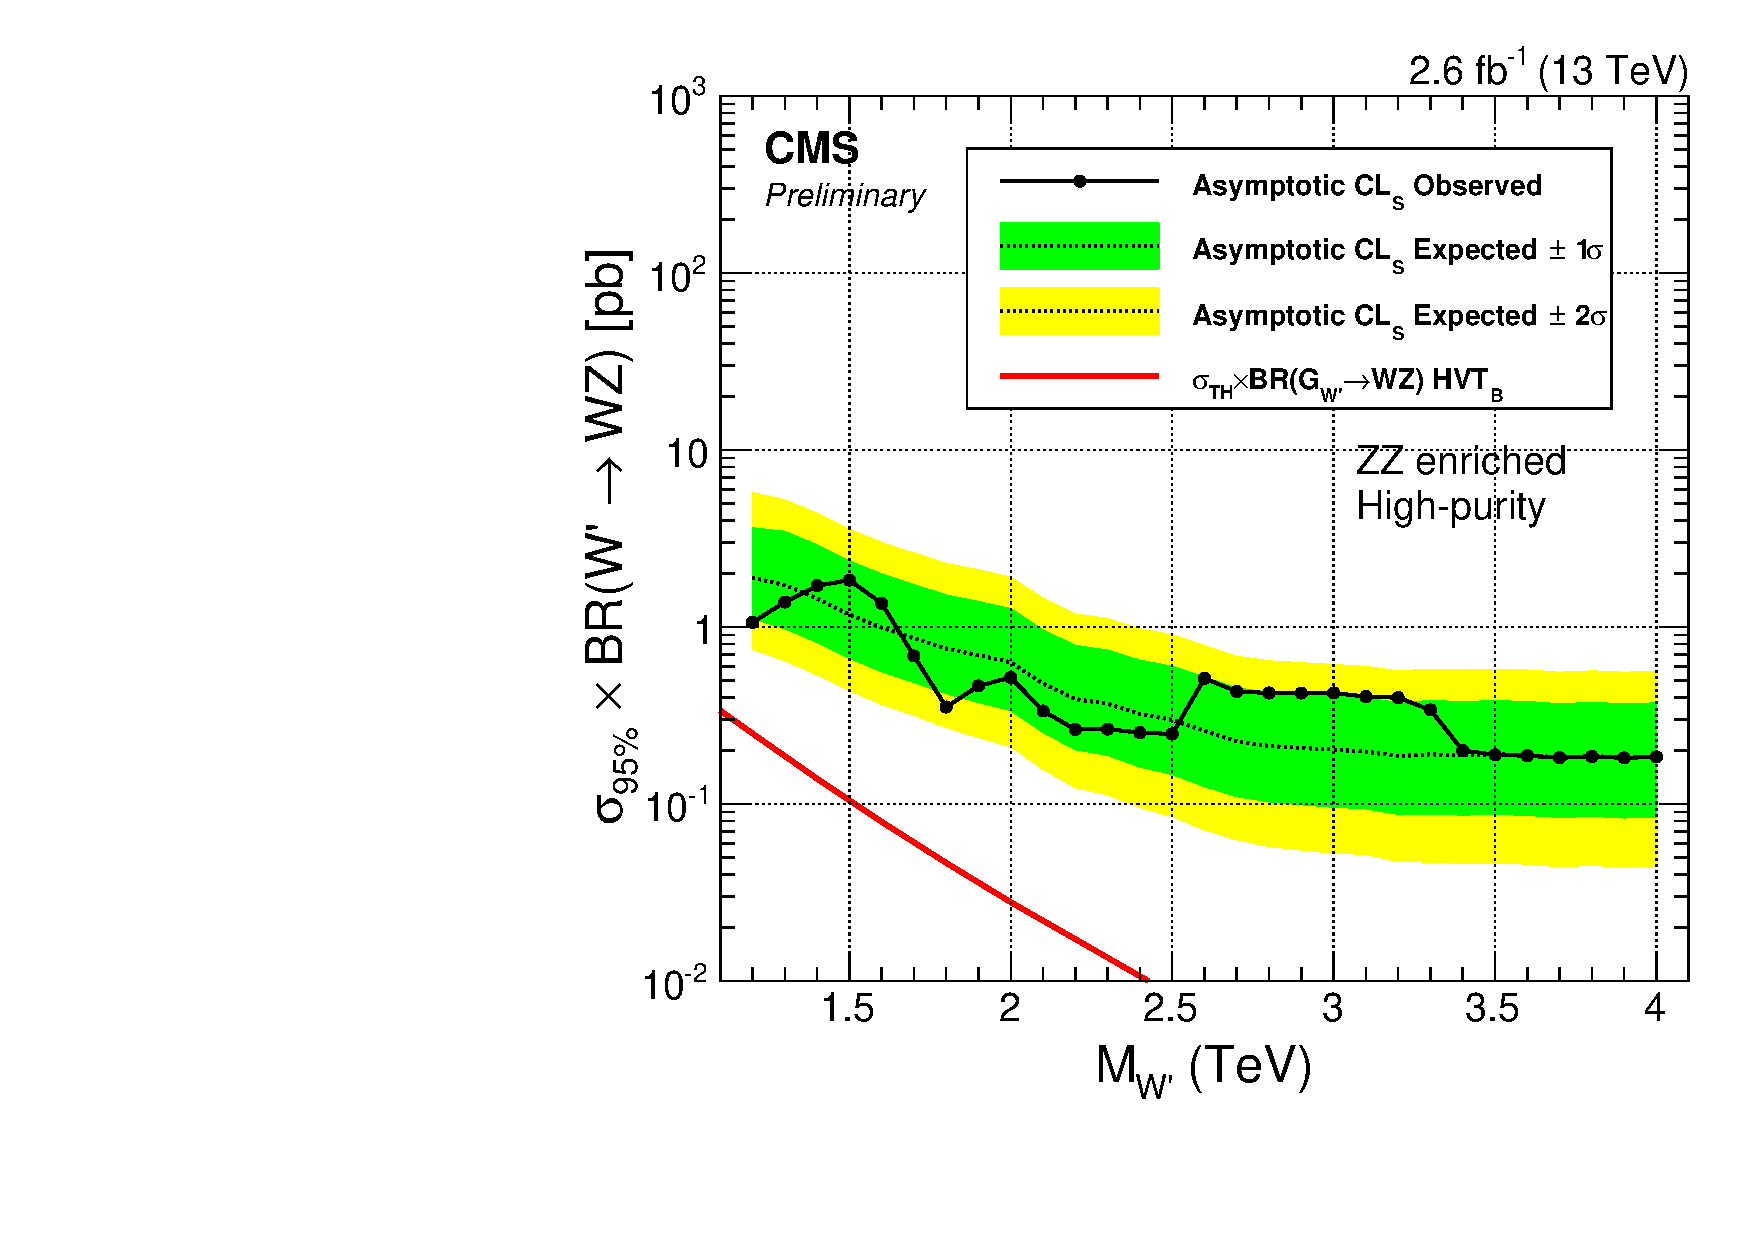
\includegraphics[width=0.32\textwidth]{figures/analysis/search1/AN-15-211/limits/brazilianFlag_WZ_ZZHP_13TeV_wPDF.pdf}\\
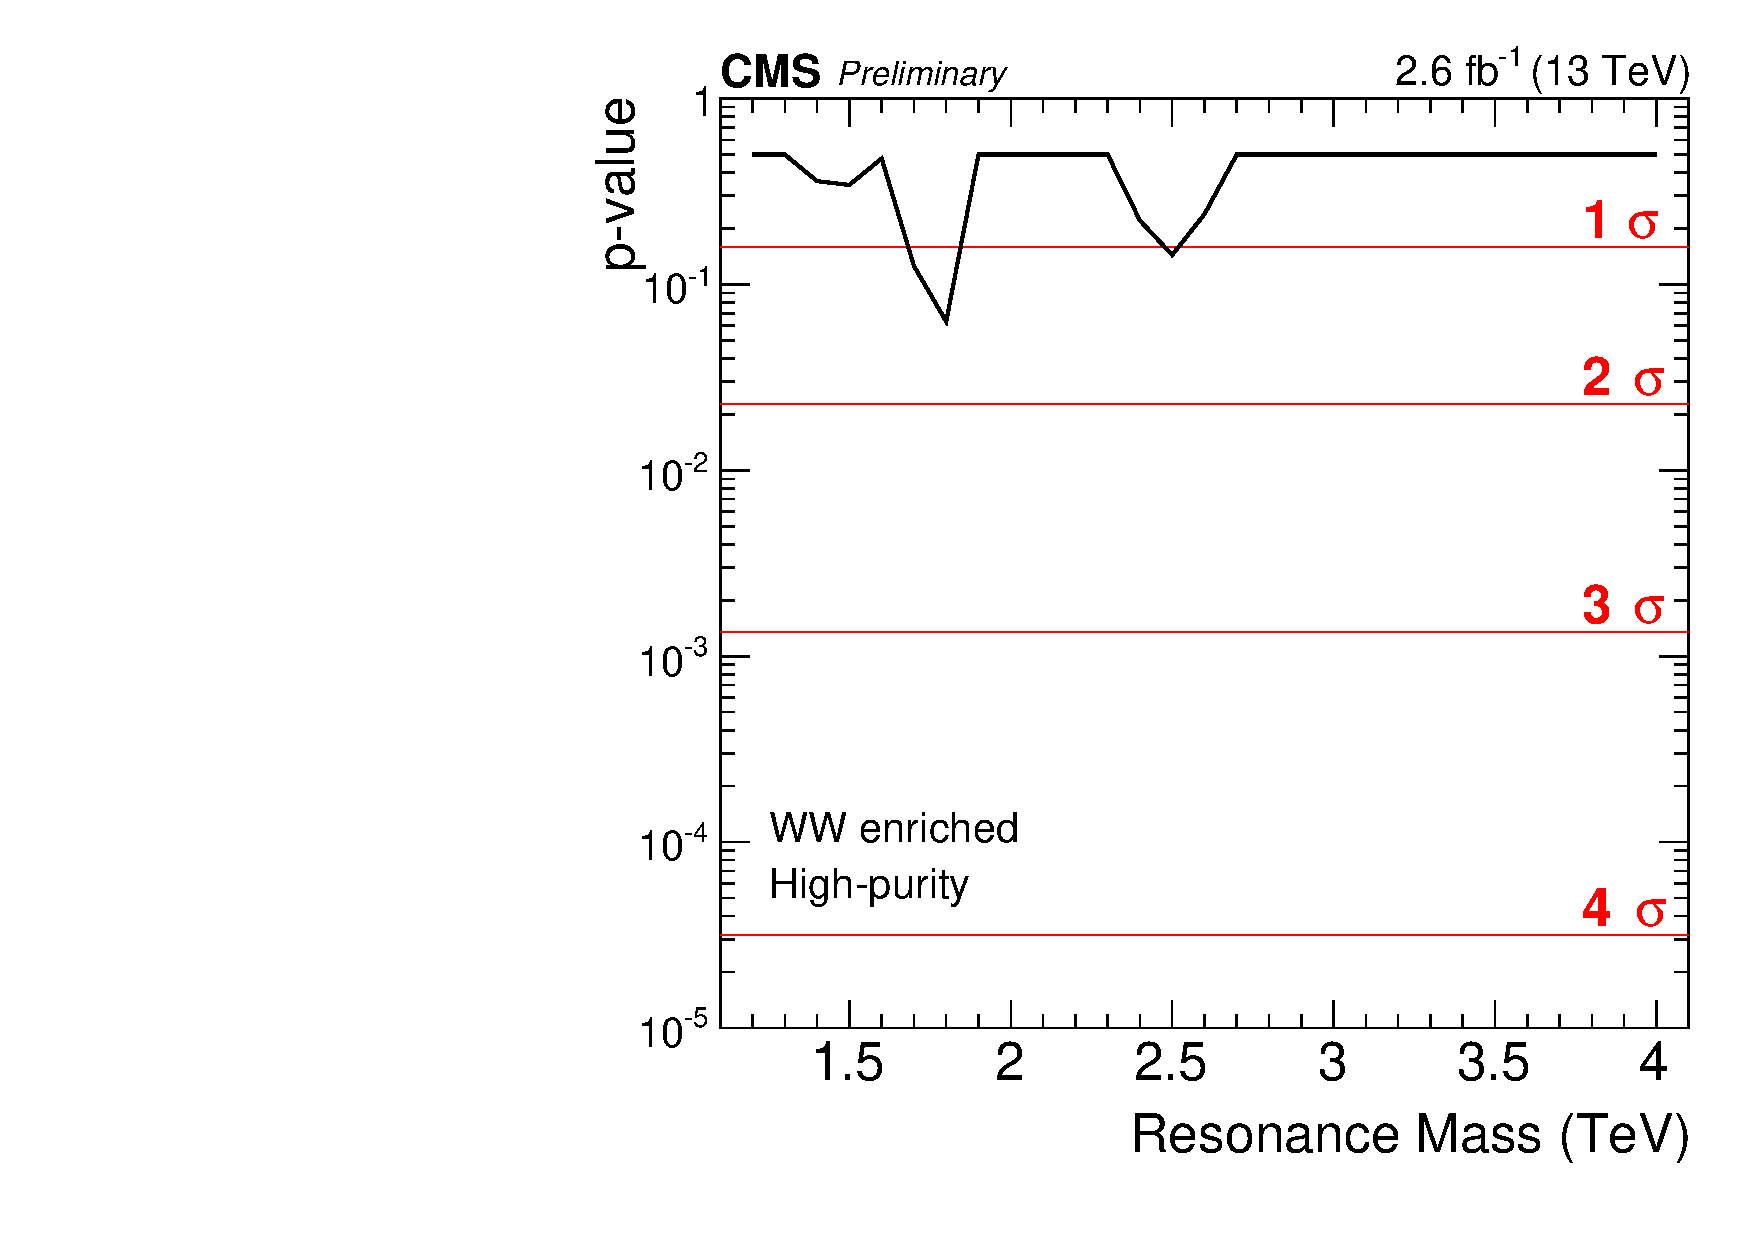
\includegraphics[width=0.32\textwidth]{figures/analysis/search1/AN-15-211/pvalues/pvalue_WZinWW_high_purity.pdf}
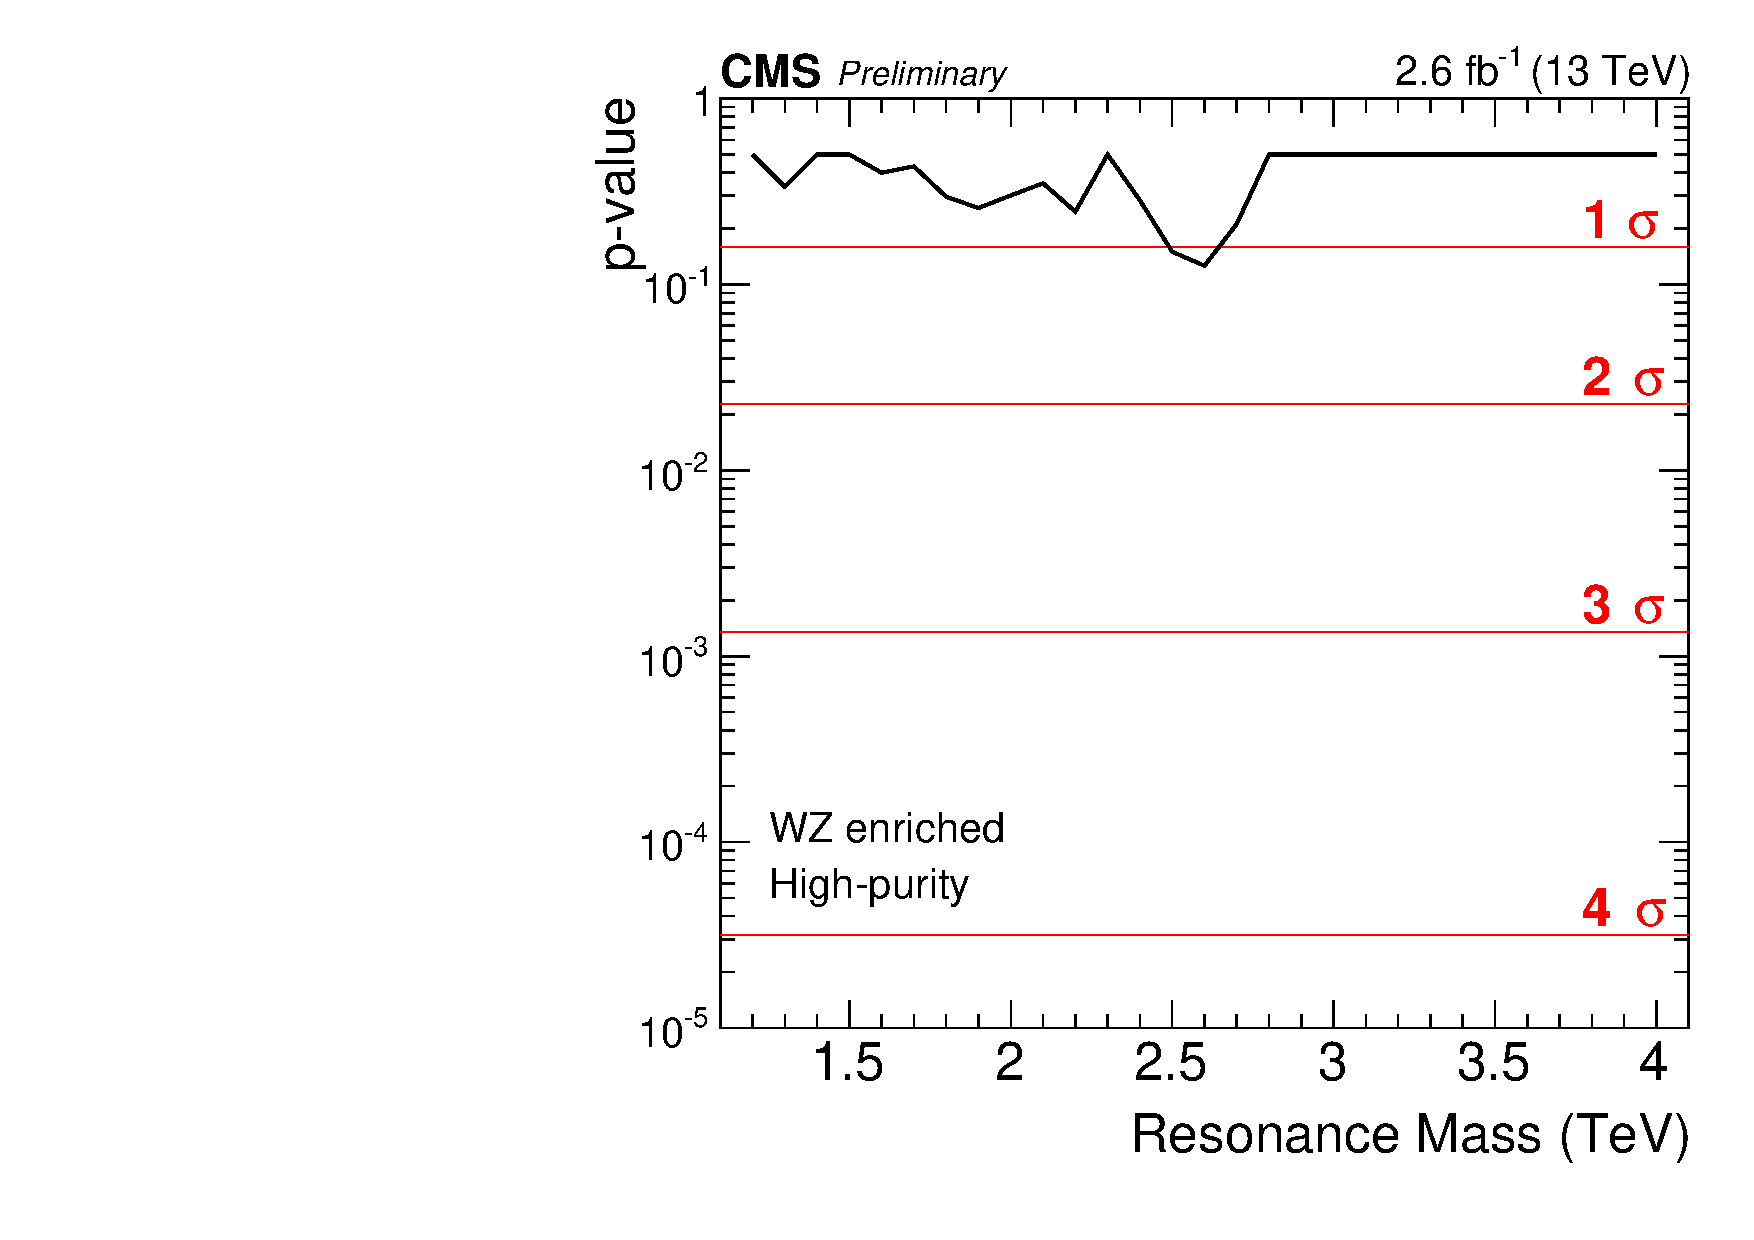
\includegraphics[width=0.32\textwidth]{figures/analysis/search1/AN-15-211/pvalues/pvalue_WZinWZ_high_purity.pdf}
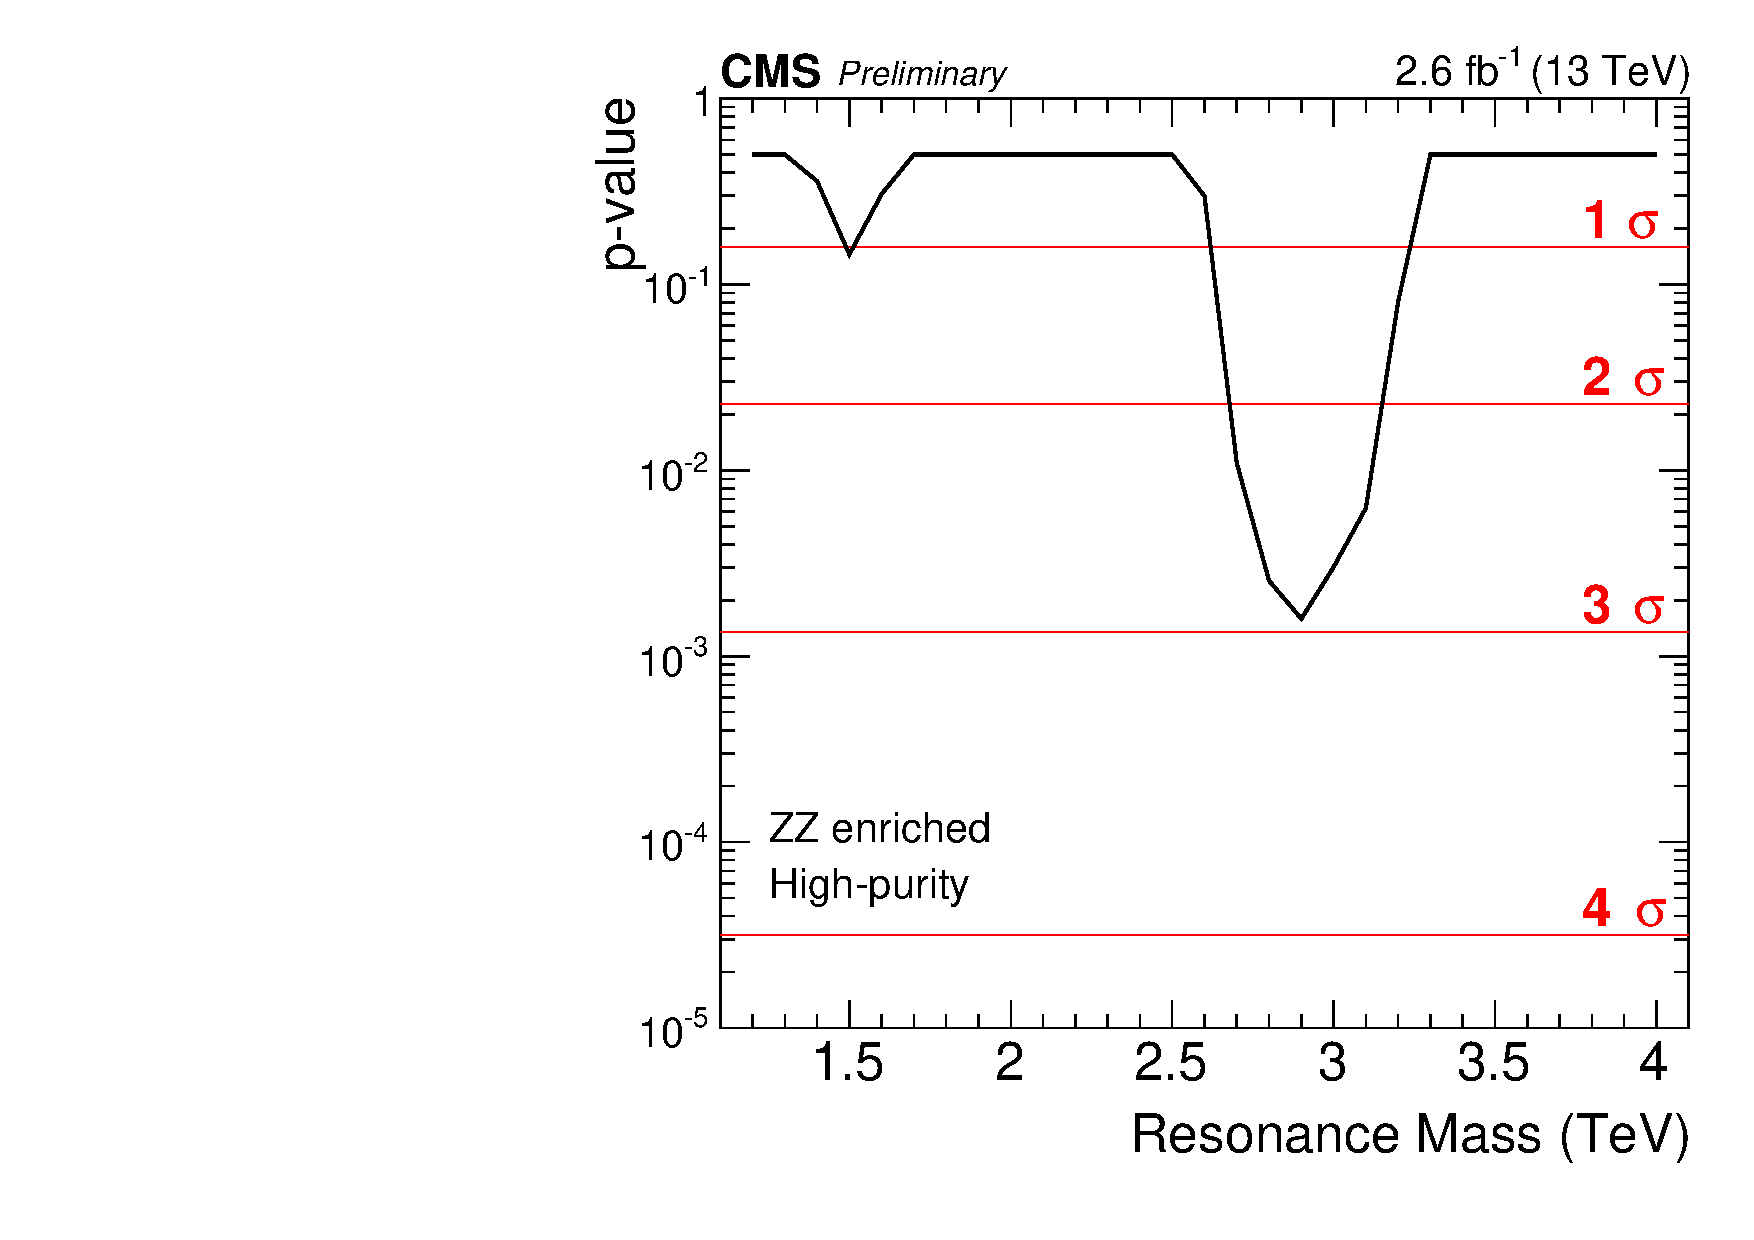
\includegraphics[width=0.32\textwidth]{figures/analysis/search1/AN-15-211/pvalues/pvalue_WZinZZ_high_purity.pdf}
\caption{Expected/observed limits and corresponding p-values obtained in the different mass categories. Here for a $W'\rightarrow WZ$ signal in the high-purity category.}
\label{fig:searchI:Limits_HPWZ}
\end{figure}


\begin{figure}[h!]
\centering
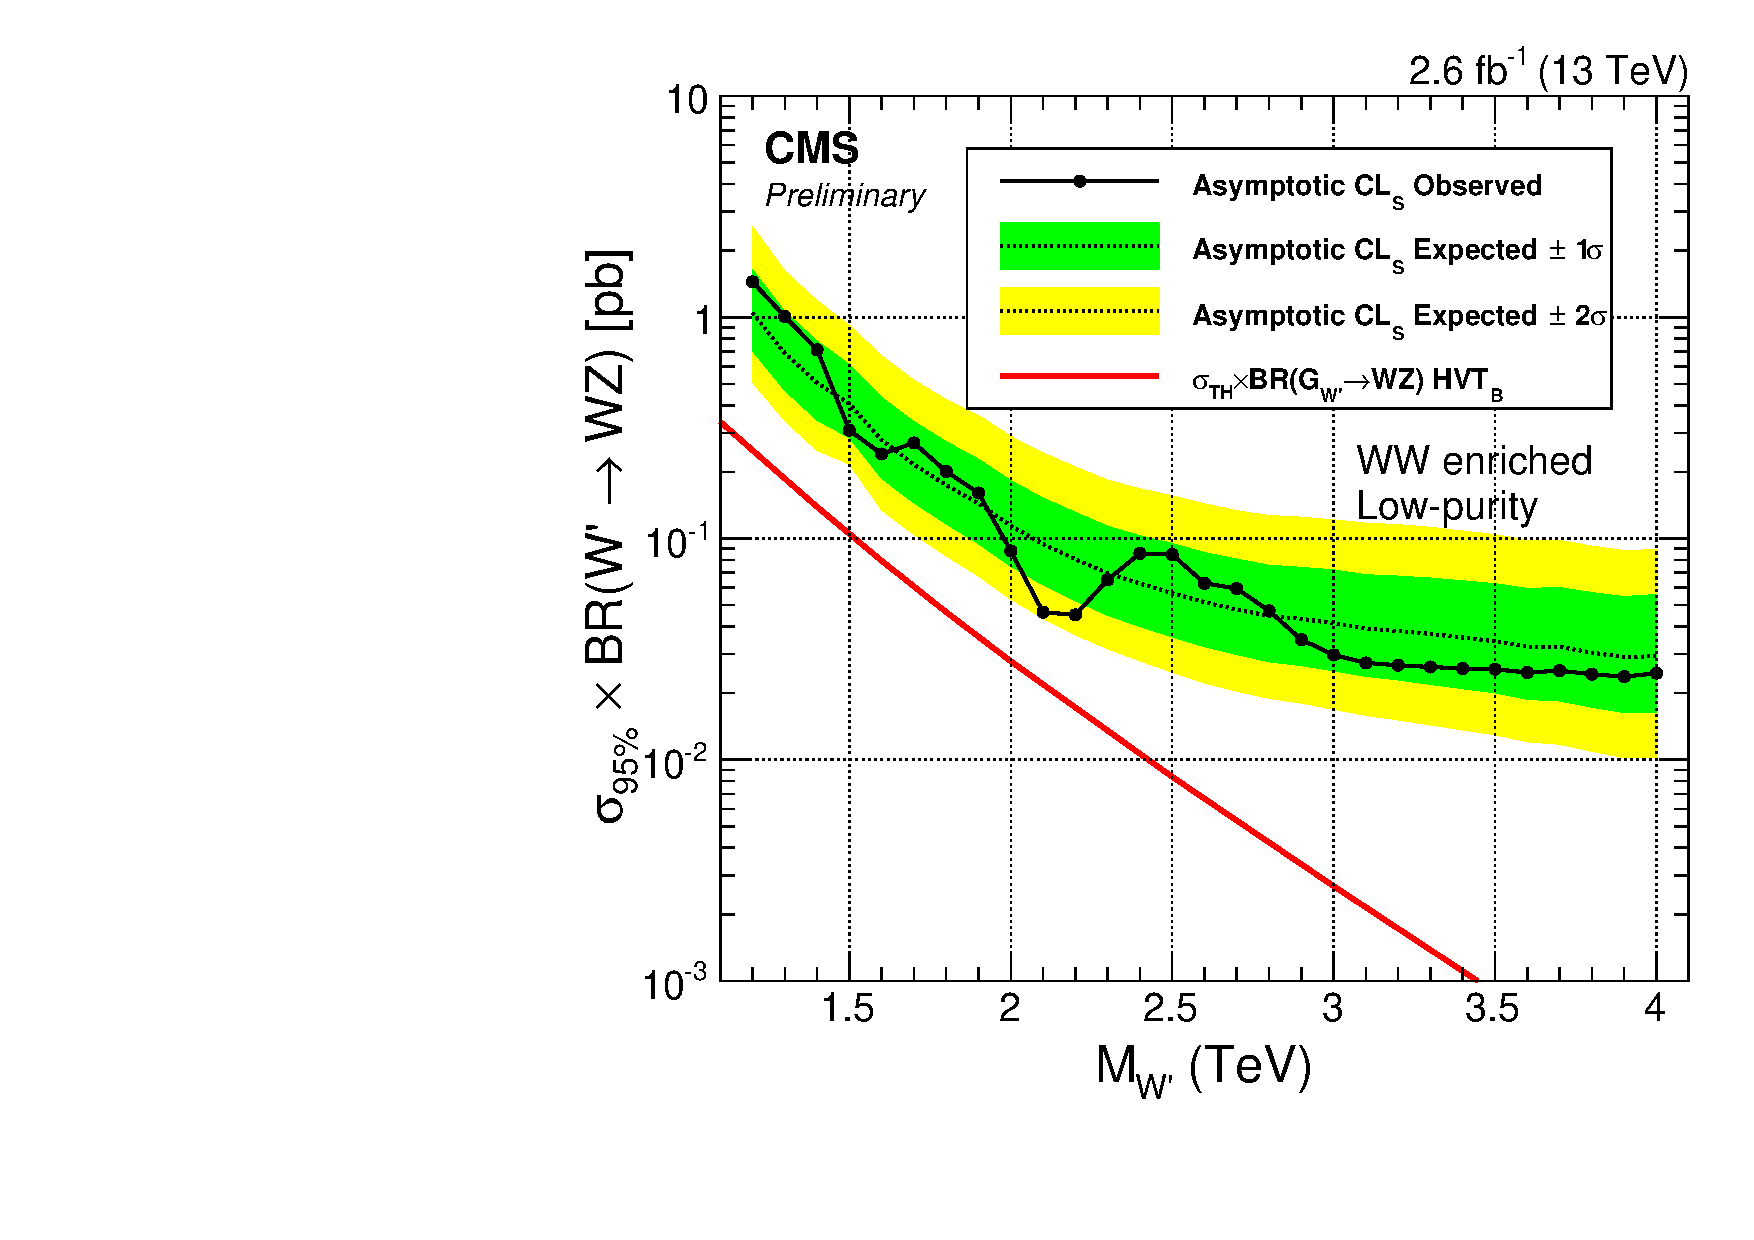
\includegraphics[width=0.32\textwidth]{figures/analysis/search1/AN-15-211/limits/brazilianFlag_WZ_WWLP_13TeV_wPDF.pdf}
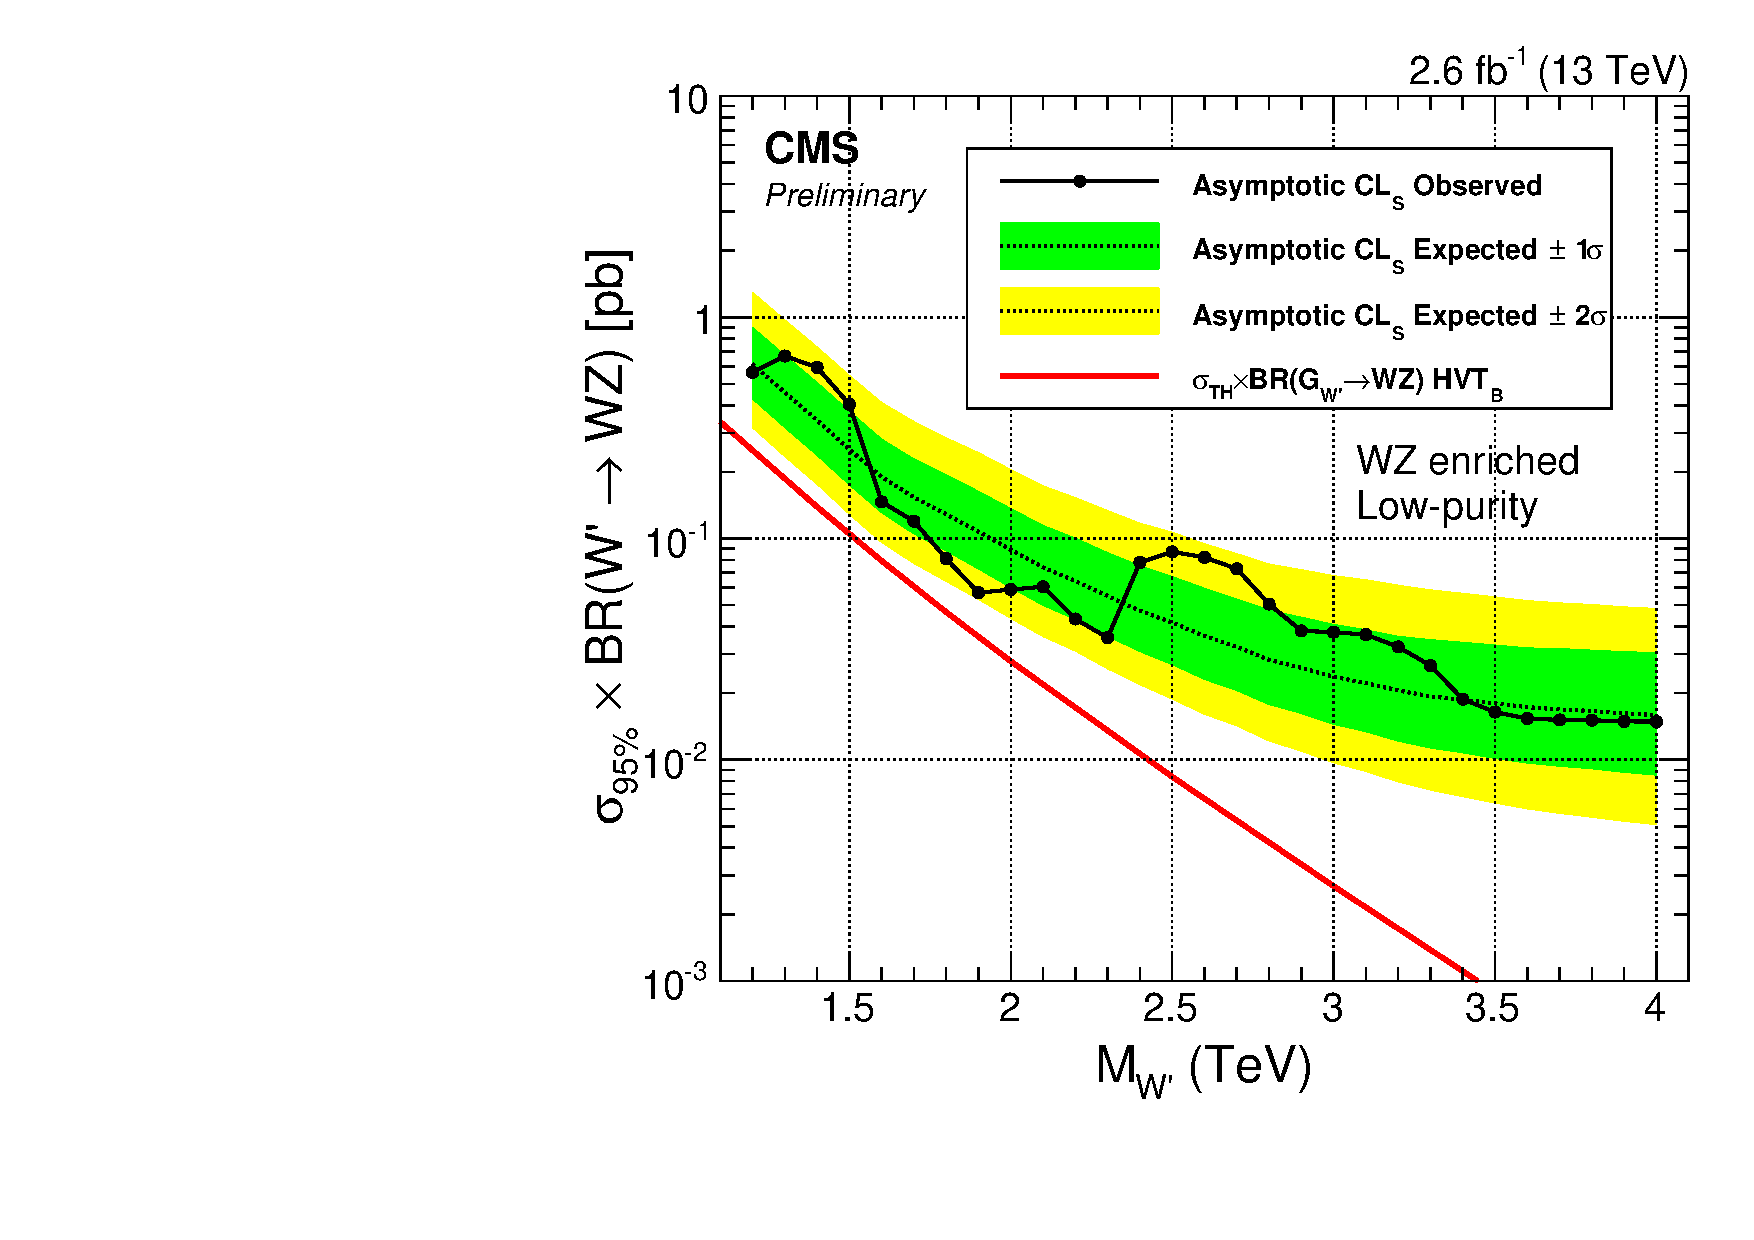
\includegraphics[width=0.32\textwidth]{figures/analysis/search1/AN-15-211/limits/brazilianFlag_WZ_WZLP_13TeV_wPDF.pdf}
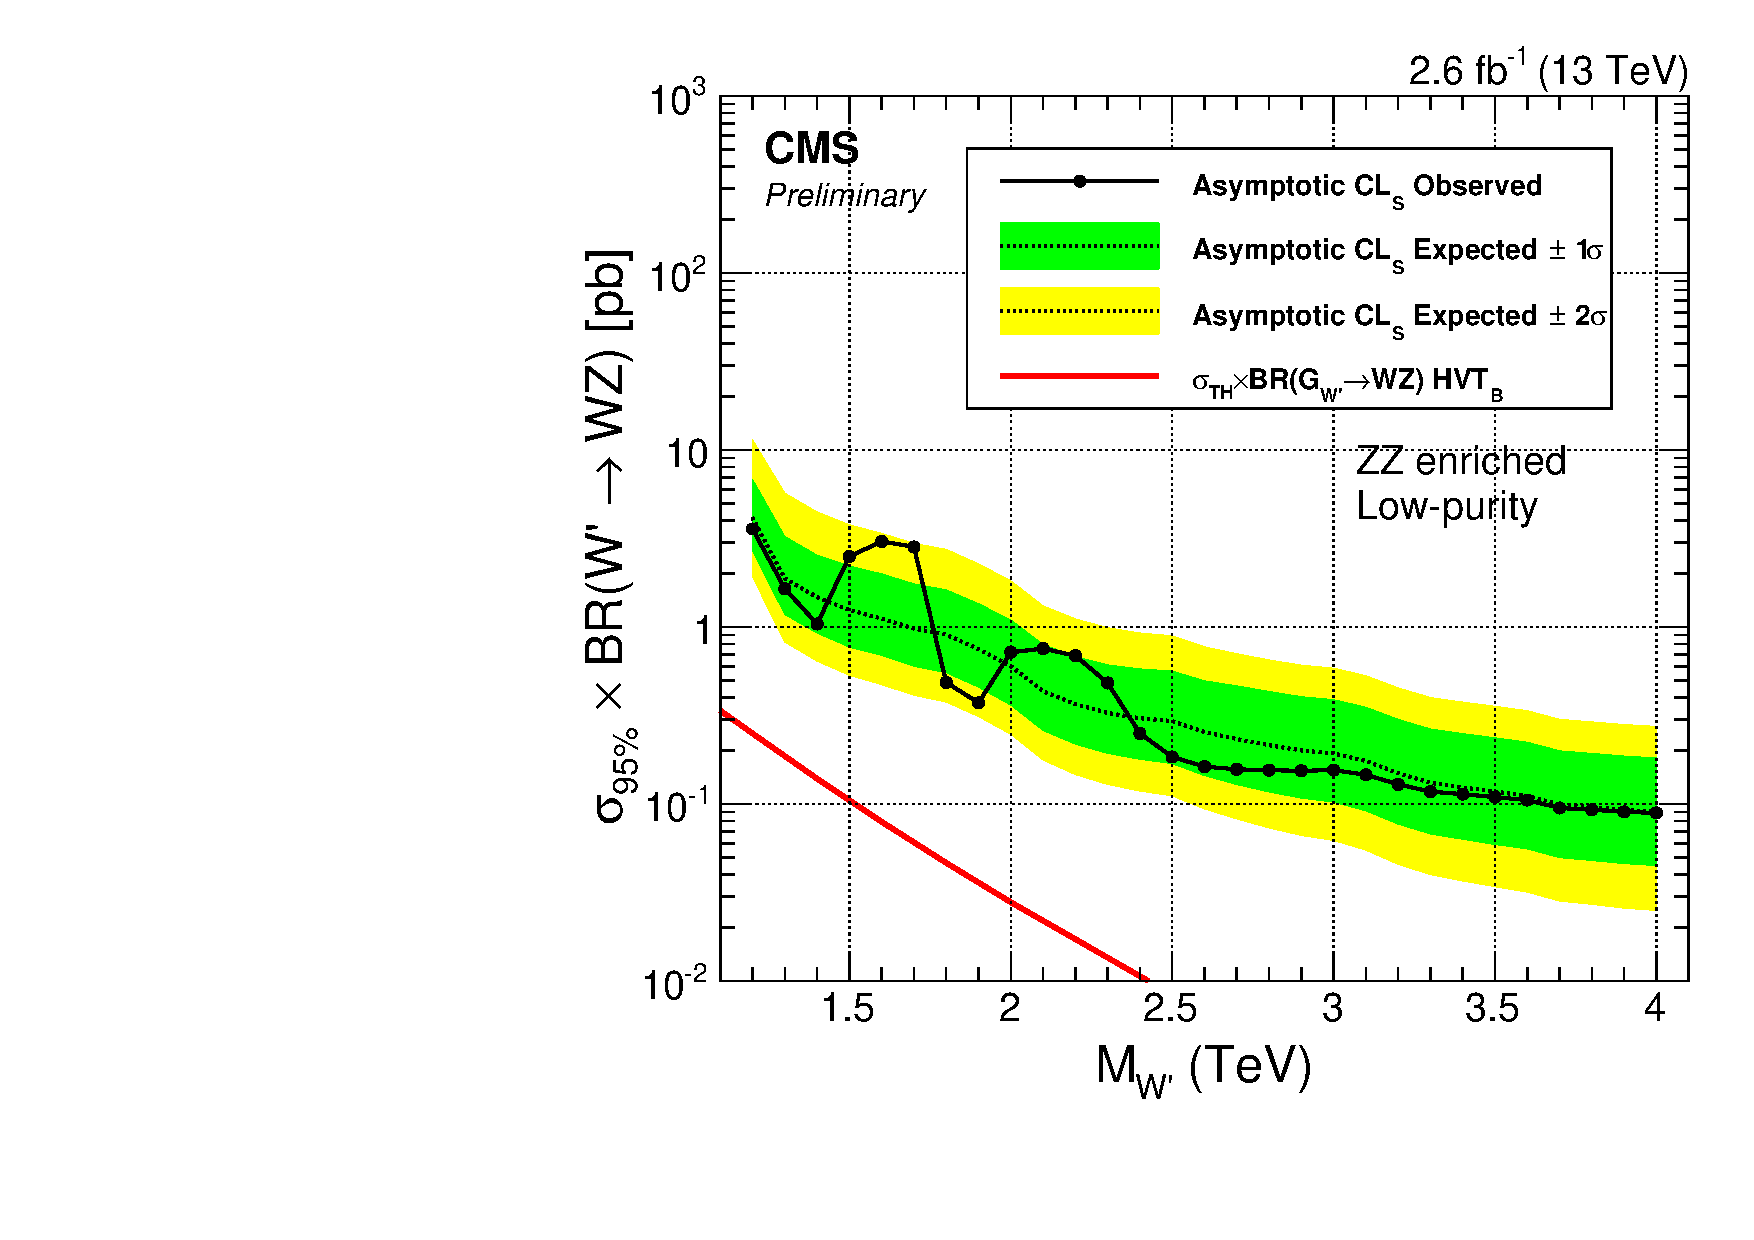
\includegraphics[width=0.32\textwidth]{figures/analysis/search1/AN-15-211/limits/brazilianFlag_WZ_ZZLP_13TeV_wPDF.pdf}\\
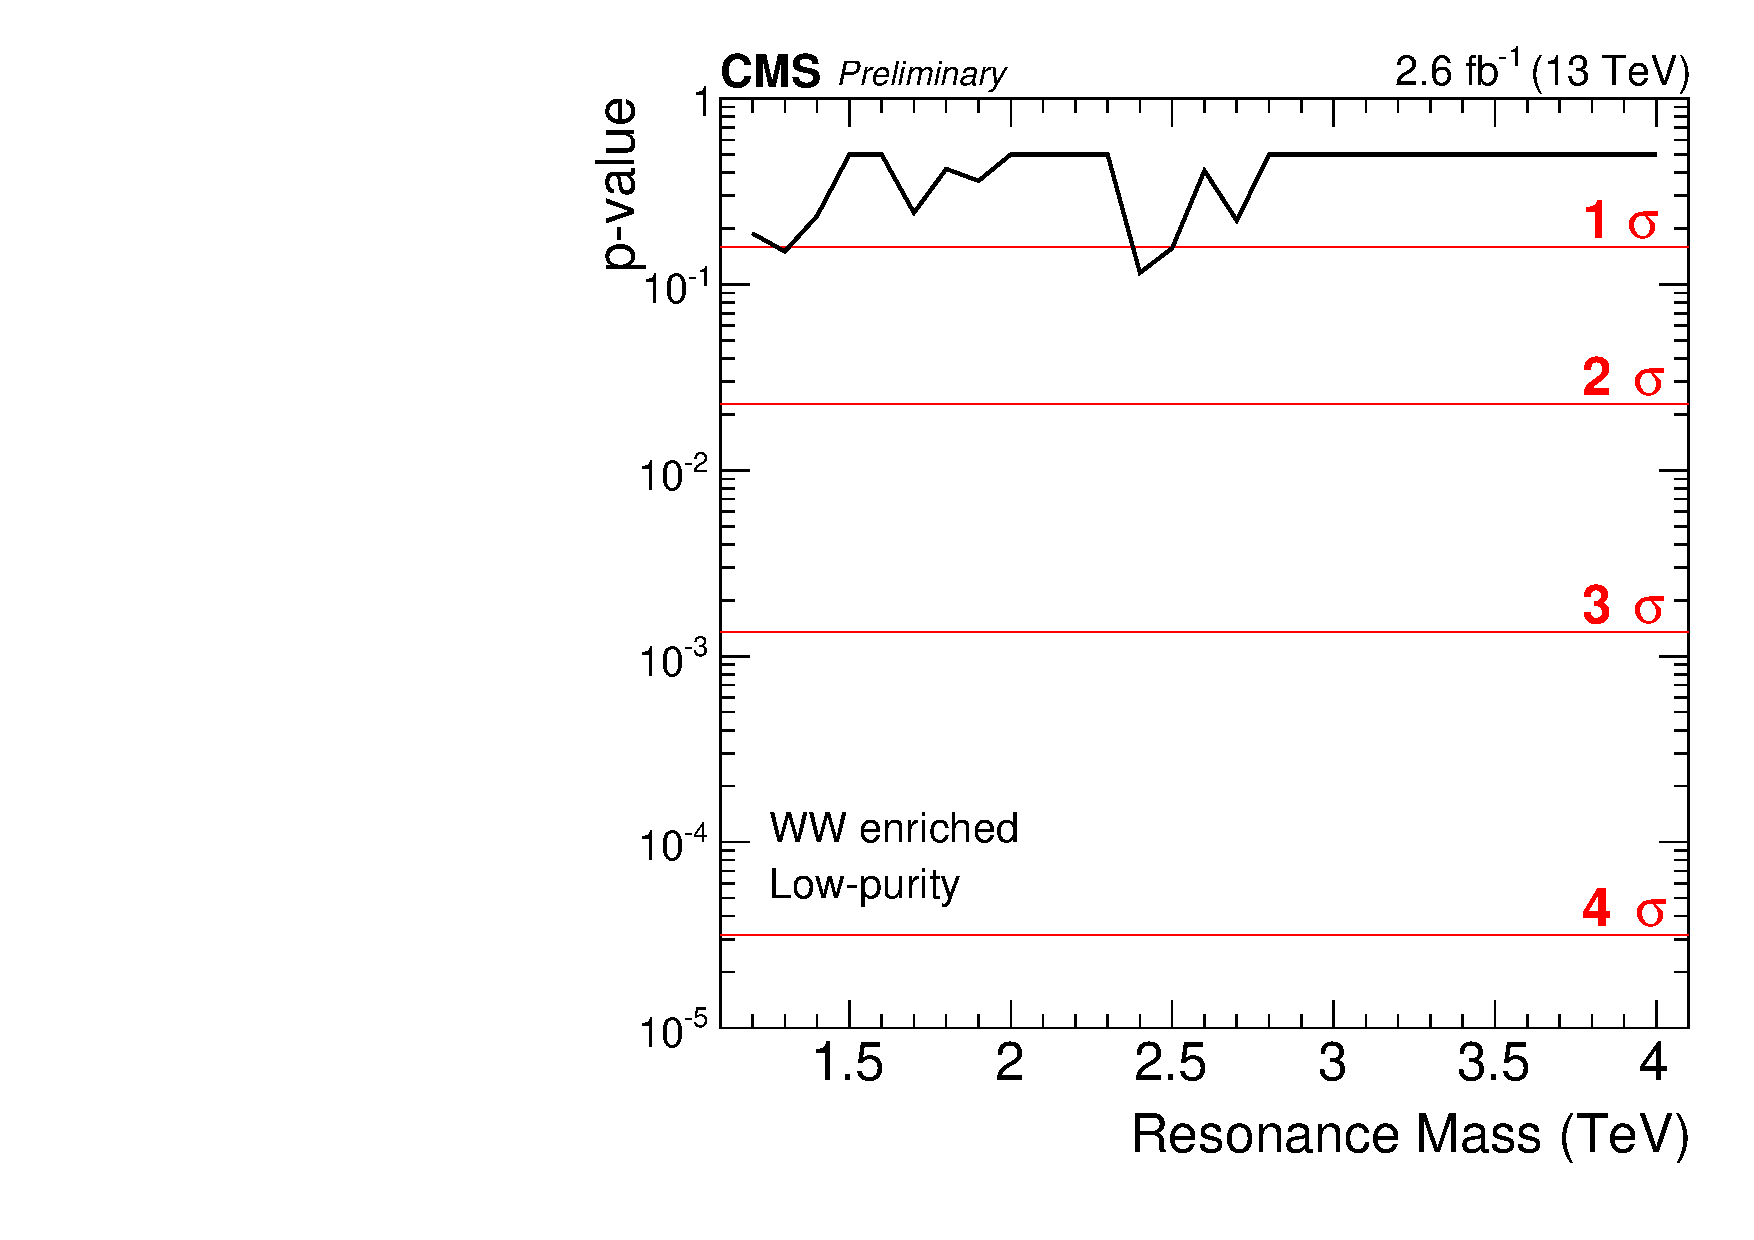
\includegraphics[width=0.32\textwidth]{figures/analysis/search1/AN-15-211/pvalues/pvalue_WZinWW_low_purity.pdf}
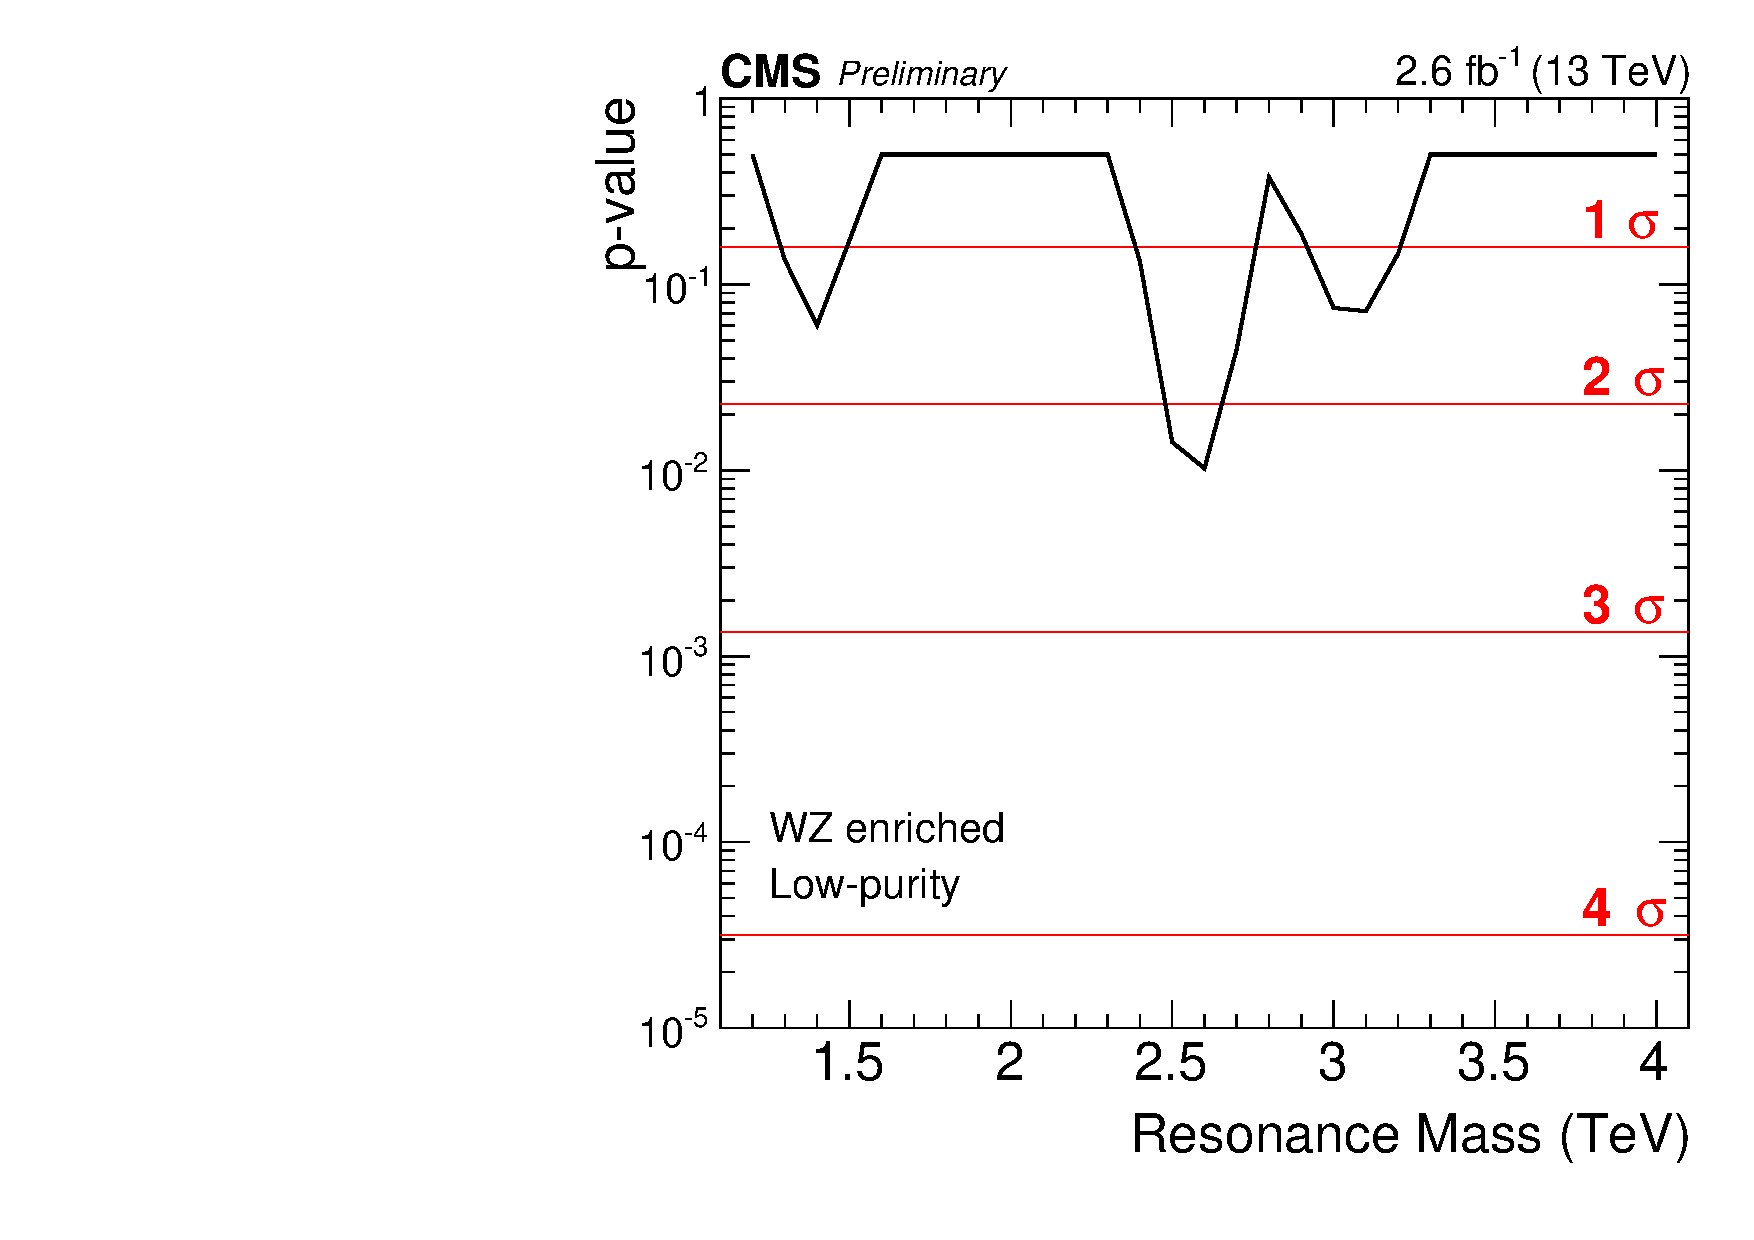
\includegraphics[width=0.32\textwidth]{figures/analysis/search1/AN-15-211/pvalues/pvalue_WZinWZ_low_purity.pdf}
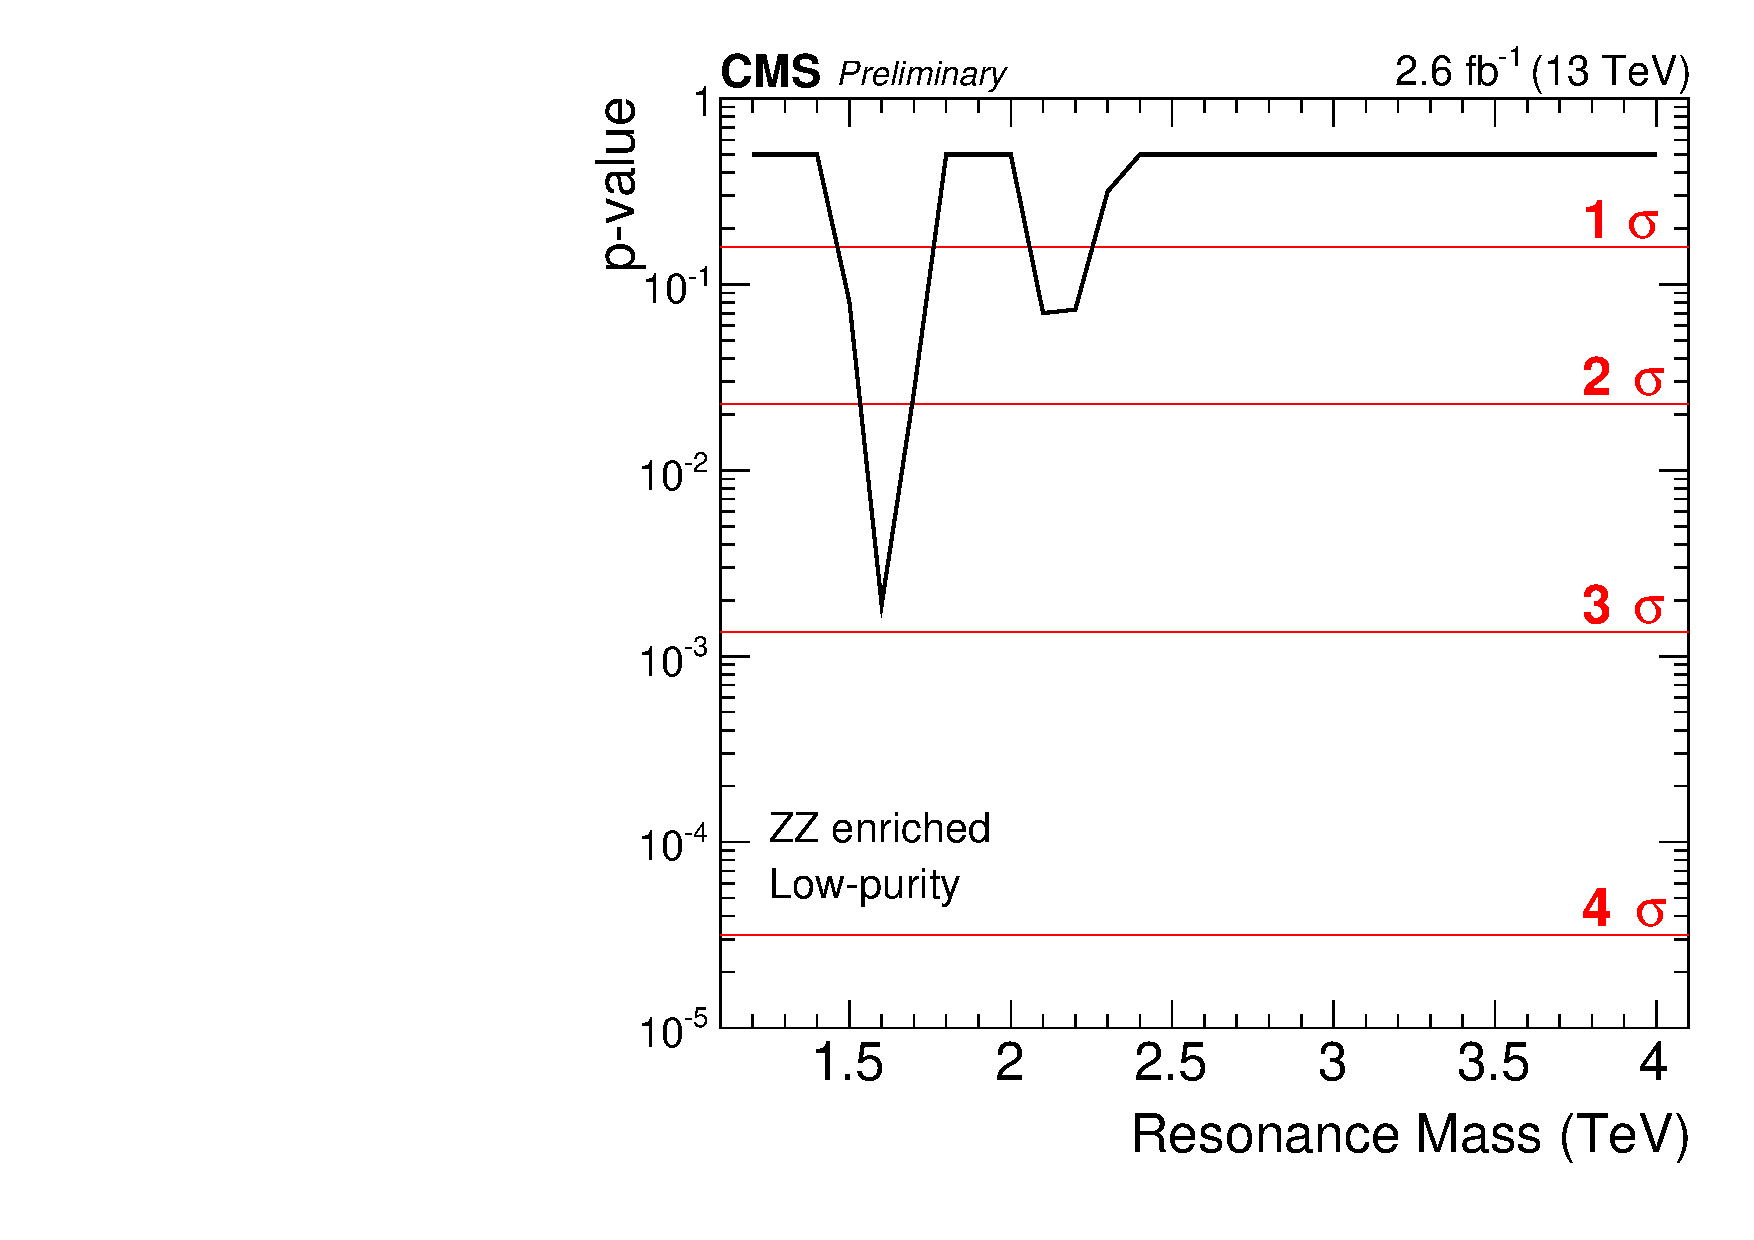
\includegraphics[width=0.32\textwidth]{figures/analysis/search1/AN-15-211/pvalues/pvalue_WZinZZ_low_purity.pdf}
\caption{Expected/observed limits and corresponding p-values obtained in the different mass categories. Here for a $W'\rightarrow WZ$ signal in the low purity category.}
\label{fig:searchI:Limits_LPWZ}
\end{figure}




\begin{figure}[h!]
\centering
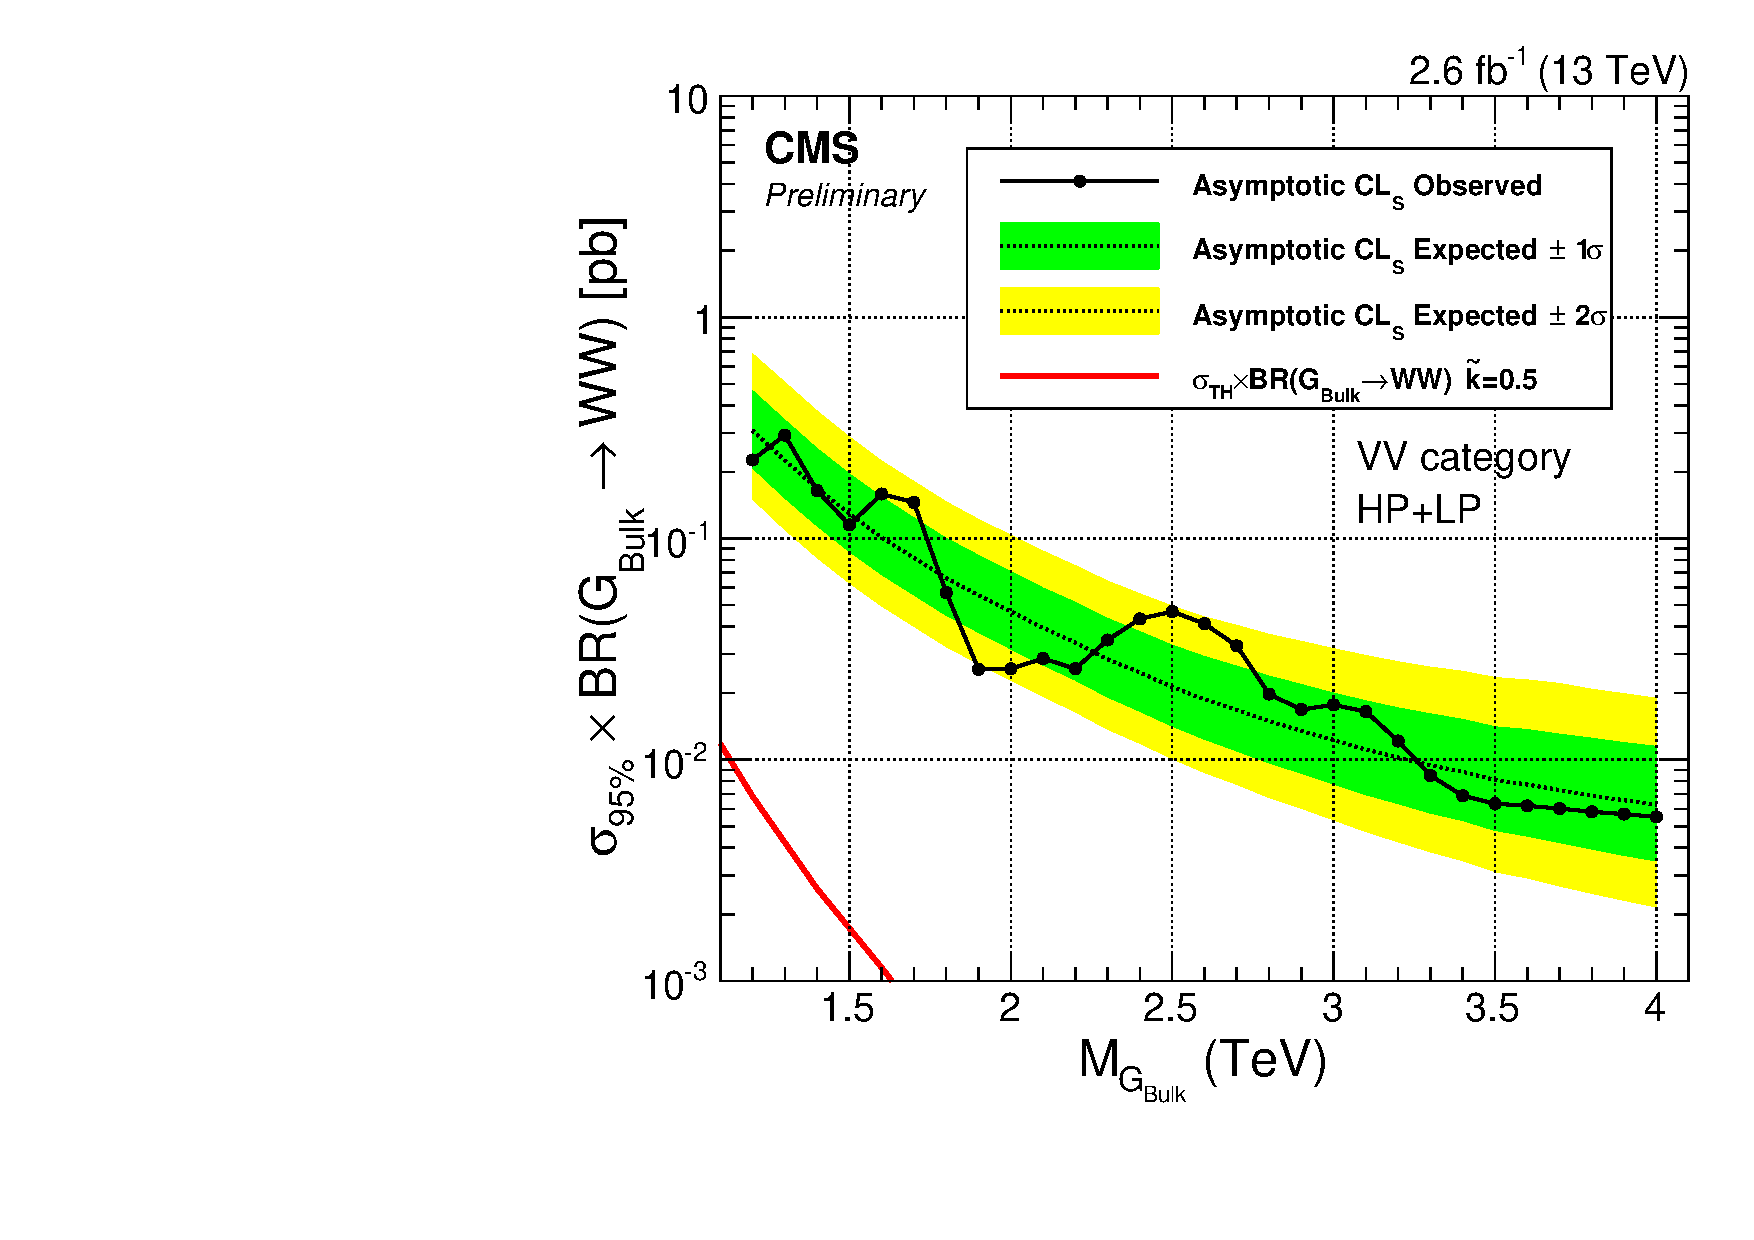
\includegraphics[width=0.32\textwidth]{figures/analysis/search1/AN-15-211/limits/brazilianFlag_BulkWW_old_combined_13TeV_wPDF.pdf}
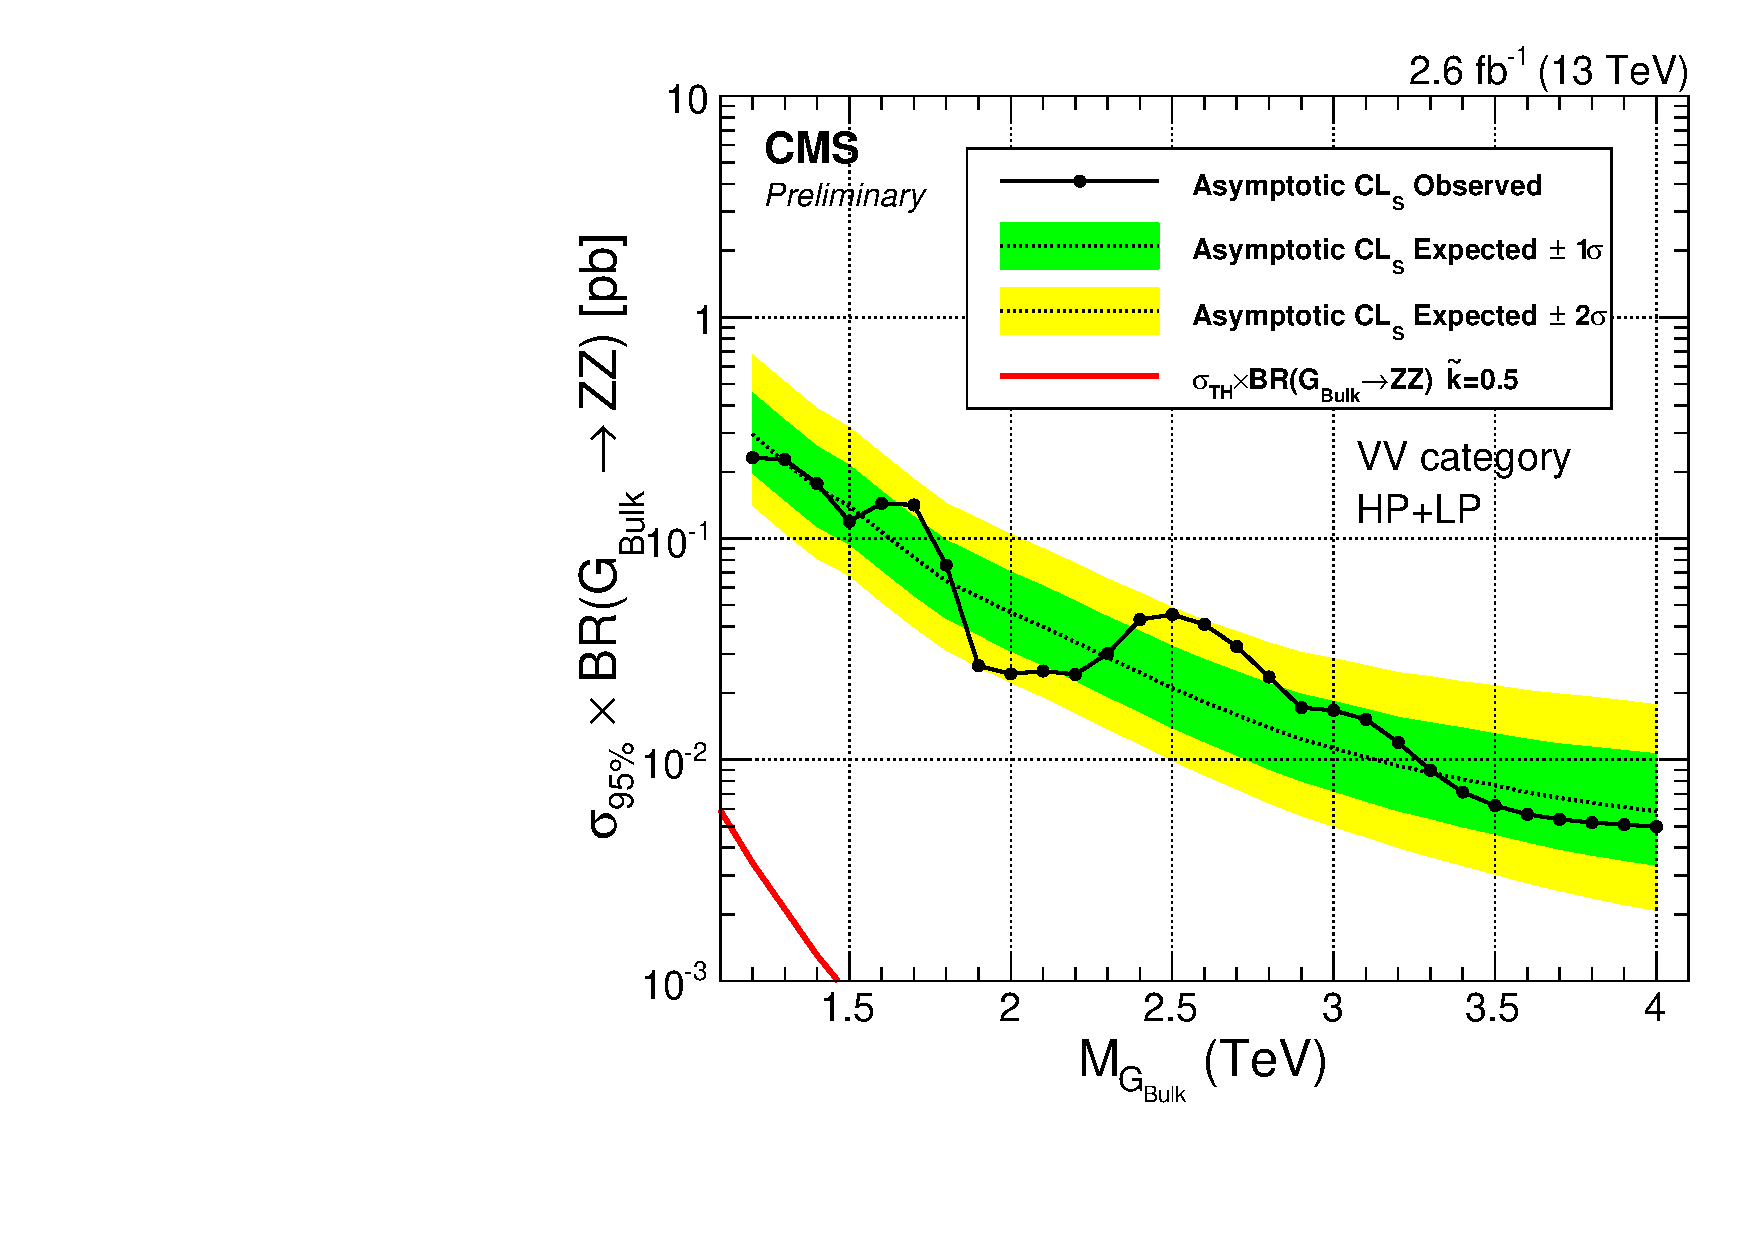
\includegraphics[width=0.32\textwidth]{figures/analysis/search1/AN-15-211/limits/brazilianFlag_BulkZZ_old_combined_13TeV_wPDF.pdf}
\includegraphics[width=0.32\textwidth]{figures/analysis/search1/AN-15-211/limits/brazilianFlag_WZ_old_combined_13TeV_wPDF.pdf}\\
\includegraphics[width=0.32\textwidth]{figures/analysis/search1/AN-15-211/pvalues/pvalue_BulkWWin_combined_old.pdf}
\includegraphics[width=0.32\textwidth]{figures/analysis/search1/AN-15-211/pvalues/pvalue_BulkZZin_combined_old.pdf}
\includegraphics[width=0.32\textwidth]{figures/analysis/search1/AN-15-211/pvalues/pvalue_WZin_combined_old.pdf}

\caption{Expected/observed limits and corresponding p-values obtained without splitting into mass categories. This analysis is performed as a cross check analysis and directly compares with the method used in the corresponding Run 1 analysis \cite{CMS-PAS-EXO-14-024}.  Here for a Bulk $G\rightarrow WW$ (left), $G\rightarrow ZZ$ (middle) and $W'\rightarrow WZ$ signal (right).}
\label{fig:searchI:Limits_CombOld}
\end{figure}


% \chapter{Data versus MC in 2015 data}
% \label{app:datamc2015}
%
% \chapter{Softdrop \PT-dependence}
% \label{app:sdptdep}
%
% \chapter{2015 cross-check analysis}
% \label{app:2015xcheck}

% figures/analysis/search1/misc/softdrop_vseta_0p8tev.pdf
% figures/analysis/search1/misc/softdrop_vseta_2p0tev.pdf
% figures/analysis/search1/misc/softdrop_wzh.pdf
% figures/analysis/search1/misc/pruned_wzh.pdf
% figures/analysis/search1/misc/gen_pruned_mass_shift.pdf
% figures/analysis/search1/misc/gen_softdrop_mass_shift.pdf